\documentclass[11pt]{article}
\usepackage{amsmath,amssymb,amsfonts,amsthm}
\usepackage[english]{babel}
\usepackage{xcolor}
\usepackage[letterpaper, margin=1in]{geometry}
\usepackage{tikz}
\usetikzlibrary{automata, graphs,positioning,chains,arrows,decorations.pathmorphing}
\usepackage{url}

\allowdisplaybreaks

% \let\bfseriesbis=\bfseries \def\bfseries{\sffamily\bfseriesbis}
%
%
% \newenvironment{point}[1]%
% {\subsection*{#1}}%
% {}
%
% \setlength{\parskip}{0.3\baselineskip}


%% USEFUL packages
%\usepackage{mypackages}

%% USEFUL macros
%% Macros Juan

\newcommand{\paths}{\text{PATHS}}

%% Macros comments
\newcommand{\tover}[1]{\textcolor{red}{#1}}
\newcommand{\td}[1]{\textcolor{blue}{[TODO: #1]}}

%% Macros logics
\newcommand{\NN}{\mathbb{N}}
\newcommand{\ZZ}{\mathbb{Z}}
\newcommand{\MM}{\mathbb{M}}
\newcommand{\SE}{\mathbb{S}}
\newcommand{\BB}{\mathbb{B}}
\newcommand{\RR}{\mathbb{R}}
\newcommand{\cF}{\mathcal{F}}
\newcommand{\cI}{\mathcal{I}}
\newcommand{\QFBILIA}{\textsf{QFBILIA}}
\newcommand{\nnf}{\textsf{f}}

\newcommand{\ite}{\textsf{ite}}
\newcommand{\limp}{\Rightarrow}
\newcommand{\flc}{\rightarrow}

\newcommand{\bagone}[1]{\llbracket #1 \rrbracket}
\newcommand{\bsingle}{\textsf{bag}}
\newcommand{\bplus}{\oplus}
\newcommand{\bminus}{\ominus}

%% Macros tools
\newcommand{\spen}{\textsc{spen}}
\newcommand{\zzz}{\textsc{Z3}}

%% Environments
\newtheorem{mythm}{Theorem}[section]
\newtheorem{mydef}[mythm]{Definition}
\newtheorem{myprop}[mythm]{Proposition}
\newtheorem{mylem}[mythm]{Lemma}
\newtheorem{myex}[mythm]{Example}
\newtheorem{mycor}[mythm]{Corollary}

\newtheorem*{myrem}{Remark} %% based on amsthm
\newtheorem*{mynota}{Notation}
\newtheorem*{mylem*}{Lemma}
\newtheorem{myclaim}{Claim}
\newtheorem*{myclaim*}{Claim}
\newtheorem*{myprop*}{Proposition}
\newtheorem*{comp}{Efficiency Study}


\newenvironment{point}[1]
{\subsection*{#1}}%
{}

\newcommand{\flist}{\text{\sc FList}}
\newcommand{\set}{\text{\sc Set}}
\newcommand{\fset}{\text{\sc FSet}}
\newcommand{\B}{\text{\bf B}}
%\newcommand{\G}{\mathcal{G}}
\newcommand{\K}{\mathcal{K}}
\newcommand{\LOG}{\text{\sc Log}}
\newcommand{\length}{\text{\rm length}}
\newcommand{\BK}{\text{\sc BK}}
%\newcommand{\cP}{\mathcal{P}}
%\newcommand{\cV}{\mathcal{V}}
%\newcommand{\cC}{\mathcal{C}}
%\newcommand{\cS}{\mathcal{S}}
%\newcommand{\cA}{\mathcal{A}}
%\newcommand{\cR}{\mathcal{R}}
%\newcommand{\cQ}{\mathcal{Q}}
\newcommand{\cG}{\mathcal{G}}
\newcommand{\cT}{\mathcal{T}}
\newcommand{\pr}{\mathbf{Pr}}
\newcommand{\Dyck}{\mathcal{D}}
\newcommand{\expected}{\mathbf{E}}
\newcommand{\bv}{\mathbf{v}}
\newcommand{\bV}{\mathbf{V}}
\newcommand{\bs}{\mathbf{s}}
\newcommand{\bsigma}{\mathbf{\sigma}}
\newcommand{\bw}{\mathbf{w}}
\newcommand{\ba}{\mathbf{a}}
\newcommand{\bq}{\mathbf{q}}
\newcommand{\bx}{\mathbf{x}}
\newcommand{\by}{\mathbf{y}}

\newcommand{\bstring}{\{0,1\}^\ast}

\newcommand{\marcelo}[1]{{\color{red} {\bf Marcelo: #1}}}
\newcommand{\etienne}[1]{{\color{blue} {\bf Etienne: #1}}}
\newcommand{\juan}[1]{{\textcolor{violet} {\bf Juan: #1}}}
\newcommand{\domagoj}[1]{{\color{green} {\bf Domagoj: #1}}}
\newcommand{\francisco}[1]{{\color{magenta} {\bf Francisco: #1}}}
\newcommand{\martin}[1]{{\color{orange} {\bf Martin: #1}}}

\newcommand{\quot}[1]{#1/\!\equiv}

\newcommand{\then}{\,|\,}
\newcommand{\body}{q}
\newcommand{\bchain}{\text{bc}}
\newcommand{\epath}{\text{path}}

\newcommand{\owner}{\text{\rm owner}}
\newcommand{\pred}{\text{\rm pred}}
\newcommand{\mine}{\text{\rm mine}}
\newcommand{\suc}{\text{\rm succ}}


\newcommand{\bP}{\mathbf{P}}
\newcommand{\bB}{\mathbf{B}}
\newcommand{\bA}{\mathbf{A}}
\newcommand{\bR}{\mathbf{R}}
\newcommand{\bS}{\mathbf{S}}
\newcommand{\bH}{\mathbf{H}}
\newcommand{\bQ}{\mathbf{Q}}

\newcommand{\forkm}[1]{F^{#1}}
\newcommand{\mfork}{F_m}
\newcommand{\mgfork}{F_{m,g}}
\newcommand{\last}{\text{\rm last}}
\newcommand{\best}{\text{\rm best}}
\newcommand{\cho}{\text{\rm choose}}

\newcommand{\ie}{i.e.$\!$ }

\newcommand{\longest}{{\text{\rm longest}}}


\newcommand{\subbody}{{\text{\rm sub-state}}}

\newcommand{\cdf}{\text{\rm {\bf DF}}}
\newcommand{\df}{\text{\rm DF}}
\newcommand{\fg}{\text{\rm FG}}
\newcommand{\fr}{\text{\rm FR}}
\newcommand{\bdf}{\text{\rm {\bf DF}}}
\newcommand{\bfg}{\text{\rm {\bf FG}}}
\newcommand{\bfr}{\text{\rm {\bf FR}}}


%\newcommand{\af}{{\rm {F_\infty}}}
%\newcommand{\baf}{{\rm {\bf F_\infty}}}

\newcommand{\af}{\text{\rm AF}}
\newcommand{\baf}{\text{\rm {\bf AF}}}

\newcommand{\pf}[1]{\text{\rm F[{#1}]}}
\newcommand{\bpf}[1]{\text{\rm {\bf F}[{$#1$}]}}

\newcommand{\cat}{\text{\rm Catalan}}


\newcommand{\gup}{{\rm {G}}}
\newcommand{\bgup}{{\rm {\bf G}}}


\newcommand{\catalan}{{\rm {\it C}}}
%\newcommand{\dyck}{{\rm {\it D}}}


\newcommand{\meet}{\text{\rm meet}}

\DeclareMathOperator*{\argmax}{argmax}


%\newcommand{\rpa}{r_p^\alpha}
\newcommand{\rpa}{r_p}

\newcommand{\ameet}{\text{\rm all-meet}}
\newcommand{\base}{\text{\rm base}}

\newcommand{\ucl}{\text{\rm up-cl}}
\newcommand{\dcl}{\text{\rm down-cl}}

\newcommand{\pol}{\text{\it P}}







%% Title
% \title{}
% \author{}
% \date{}

\begin{document}
	
	% \sloppy
	% \maketitle
	
	%!TEX root = focs.tex

\section{Introduction}

The Bitcoin Protocol \cite{Bitcoin} presented in October 2008 by the anonymous Satoshi Nakamoto, also known as the Blockchain Protocol or the Nakamoto Protocol, introduces a novel decentralized network-consensus mechanism that is trustless and is open for anyone connected to the internet. Moreover, it allows participants to leave and re-join the network at will. To support such an open and dynamic topology the protocol requires an underlying currency (a so-called \emph{cryptocurrency}) to encourage/discourage participants to/from taking certain actions. The largest network running this protocol is the Bitcoin network, and its underlying cryptocurrency is Bitcoin (BTC). As of March 2018, Bitcoin is the most successful cryptocurrency with a value per coin of about 8.100 USD~\cite{BitcoinPrice} and almost 17 million coins in circulation~\cite{Totalcoins}.
 
Following the success of Bitcoin, several new cryptocurrencies have been created. Some of them are simple replicas of Bitcoin with slight modifications on the protocol parameters (e.g. Litecoin~\cite{Litecoin} or Bitcoin Cash~\cite{Bcash}), while some of them introduce interesting new modifications on top of the protocol to provide further functionalities (e.g. Ethereum~\cite{Ethereum} or Monero~\cite{Monero}). Also, there are several tokens that are usually called cryptocurrencies but are either centrally controlled or simple Ponzi schemes without a real cryptocurrency behind. Considering some of the latter, to this day more than 1500 cryptocurrencies have been issued~\cite{coinmarketcap}.

But despite the success and popularity of cryptocurrencies, the foundational aspects of their rulling protocol are far from fully understood. As has been claimed before \cite{mininggames:2016}, the Bitcoin Protocol involves many actors and incentives, making it rather hard to formalize and study rigorously. A good body of research pursuing this objective has been presented recently (see e.g.~\cite{mininggames:2016,optimalselfishmining2017,instabilitywithoutreward:2016}), yet there are still some fundamental aspects of the protocol that are important and have not been considered. In this paper, we present a formal model that takes some of these aspects into consideration. Before presenting our contributions and discussing some related work, we give a brief introduction to the Bitcoin Protocol.

\paragraph{\bf The Bitcoin Protocol.} The objective of the Bitcoin Protocol is to generate consensus on a data structure that is shared among all nodes in a trustless and decentralized peer-to-peer network, in such a way that everyone (not only participants of the network) can verify the integrity of the complete data structure without trusting other nodes. Moreover, the network is open for anyone to participate, and nodes can leave and re-join the network at will. To achieve consensus under these conditions, the Bitcoin Protocol requires the shared data structure to be an append-only record of transactions. The inclussion of new transactions to this data structure works as follows: every node that wants to include new transactions must communicate these transactions to their neighbours, who will in turn communicate them with their neighbours, and so on. Transactions are then spread throughout the network via so-called \emph{peer-to-peer whispering}. Naturally, at any point in time every node in the network will have received a set of transactions. Note that there is no guarantee regarding who received which transaction, so these transactions are not considered valid yet. Eventually, one node will be \emph{allowed} (we will explain this in detail later) to form a new \emph{block} and present it as a candidate to extend the data structure. The block will contain some of the transactions received by that node, plus a pointer to some previous block (concretely, the hash value of its header). The newly formed block is then spread throughout the network, also in a whispering fashion. Since every block points to a previous block, a tree of blocks is naturally formed. The consensus data structure is defined as the longest branch of such tree, which is known as the \emph{blockchain}.

To make the dynamics described above work in a trustless and decentralized network with adversaries, the Bitcoin Protocol requires an underlying currency to encourage actors in the network. The first and most important incentive is for the generation of new blocks. Whenever a node forms a new block, the node is rewarded with a certain amount of currency. This amount was originally 50BTC and halves every approximately four years, which is informaly known as Bitcoin's \emph{deflation}; the reward is currently 12.5BTC. The currency generated in a block can only be spent whenever the new block contains at least 100 descendants in the tree and forms part of the blockchain. Therefore, whenever a node forms a new block, he is encouraged to place this block in a part of the tree with a high probability of becoming part of the blockchain. Actually, the protocol states that new blocks should always be appended on top of a block with maximal distance to the root of the tree.

Since blocks give reward, every node naturally wants to generate blocks. If we expect the currency to have any value, generating new blocks must then be hard. A block is called \emph{valid} by the protocol if its hash value (in practice, the hash value of its header), when interpreted as a number, is less than a certain threshold. Since hash functions are pseudo-random, the only way to generate a valid block is to try with several different blocks, until one of them has a hash value below the established threshold. This is known as \emph{mining}, and the number of (valid and invalid) blocks per second that a miner can hash is called his \emph{hash power}. Nodes who participate in the generation of blocks (which are in practice very few) are called \emph{miners}. It is important to mention that if a miner sends an invalid block to the network, the protocol states that other nodes should not spread it. Therefore it will not become part of the blockchain.

Assume now that a miner generates a new valid block $A$ that points to the last block of the current blockchain. He will try to get this new block spread accross the network as fast as possible, because this makes the branch of such block longer encouraging other nodes to mine on top of this new block. If he keeps this block private, most likely other miners will generate a longer branch without his node, and he will not be able to place his block in the blockchain, missing the associated rewards.

The other important incentive is for including transactions. Why would a miner include the transactions he has received into a new block? He might just decide to include few of them. To solve this, the protocol establishes that transactions can include a \emph{fee}. The fee of all transactions in a block plus the block reward is the total amount of currency earned by the miner who generated the block. To control the practical growth of the blockchain, every block has a maximum size (in Bitcoin it is 1MB). The miner is naturally encouraged then to choose a subset of the transactions he has received to maximize his reward. It is important to note that the vast majority of the currency earned by miners comes currently from the block reward; in current Bitcoin blocks, fees rarely exceed 10\% of the block reward.

\paragraph*{\bf Contributions.} From the description above, it is clear that miners are in practice competing for generating new blocks that will (in the long run) form part to the blockchain. This can be naturally studied from a game-theoretical perspective to understand the expected behavior of \emph{rational} miners. As mentioned above, the protocol proposes the simple strategy of appending new blocks to the top of an arbitrary branch of maximum length (usually only the blockchain) which is known as the \emph{default strategy}. CONTINUE HERE


\paragraph*{\bf Related Work.} The first game-theoretical formalization of the Bitcoin mining dynamics was presented by Kroll et al. \cite{economics_of_mining2013}, who showed that in the full-disclosure game there is a Nash equilibrium whenever all miners adopt \emph{monotonic} strategies. Eyal and Sirer~\cite{selfishmining2014} introduced a different strategy known as \emph{selfish mining}, in which miners withhold found blocks under certain conditions. Their main result is that a miner with strictly less than 50\% of the network's hash power can \emph{produce} a proportion of the blocks in the blockchain that is higher than his proportion of the network's hash power, assuming that all other miners are following the default strategy (thus proving that the default strategy is not a Nash equilibrium). A good body of work has extended selfish mining. Notably, in \cite{optimalselfishmining2017} the authors present a generalization that is formalized by means of Markov Decision Processes and prove that selfish mining can be further optimized. In \cite{stubborn_mining:2016} selfish mining is analyzed in combination with Eclipse Attacks~\cite{eclipseattacks2015}. Further studies have been carried in efforts to prevent miners from adopting selfish strategies (e.g. \cite{stop_selfish_mining2014,selfishmining2014}). The work around selfish mining differs from our work in that the model they consider assumes all blocks to have the same reward, meaning there is no \emph{deflation} and no discount is considered by miners. Carlsten et al. \cite{instabilitywithoutreward:2016} studied the \emph{tail} behavior of Bitcoin in which the block reward becomes negligible compared to the mining fees. They prove that in such situation miners have further incentives to deviate from the default strategy. The reason is that the probability of losing the reward because of a block not forming part of the blockchain is outweithed by the increase in reward for including high-fee transactions that were already in previous blocks. This work differs from our's in that their model considers as block reward only the transaction fees. Under a model that considers network connectivity, two strategies that are superior to the defalut one are presented in \cite{bitcoin_attacks_2013}. In \cite{ddos_attacks2014,empirical_dos_attacks2014} the authors study the feasibility of earning an \emph{unfair} number of blocks by deploying DDOS attacks against other miners. This is somehow orthogonal since we do not consider practical aspects of the network. 



	%!TEX root = focs.tex

\section{A Game-theoretic Characterization of Bitcoin Mining}
\label{sec-formalization}

The mining game is played by a set $\bP = \{0, 1, , \ldots, m-1\}$ of players, with $m \geq 2$.
In this game, each player has some reward depending on the number of blocks she owns. Blocks are placed one on top of another, starting from an initial block called the {\em genesis block}. Thus, the game defines a tree of blocks. Each block is put by one player, called the {\em owner} of this block. Each such tree is called a {\em state of the game}, or just {\em state}, and it represents the knowledge that each player has about the blocks that have been mined thus far. 

The key question for each player is, then, where do I put my next block? In bitcoin, miners are only allowed to spend their reward as long 
as their blocks belongs to the \emph{blockchain} of a state, which is simply the longest chain of blocks in this state. Thus, players face essentially two possibilities: they can put their blocks right after the end of the longest chain (the blockchain), or they can try to \emph{fork} 
from the longest chain, betting that they will be able to put enough blocks to turn a smaller chain into the blockchain. As the likelihood of 
mining the next block is directly related to the comparative hash power of a player, it makes sense to model this game as an infinite 
stochastic game, in which the probability of executing the action of a player $P$ is given by her comparative hash power. 

Let us now turn to the formal definition of the game. 

\medskip
\noindent
\textbf{Blocks, states and blockchain}. In a game played by $m$ players a block is a string $b$ over the alphabet $\{0,1,\ldots, m-1\}$. We denote by $\bB$ the set of all blocks, that is, $\bB = \{0,1,\ldots , m-1\}^*$. Each block apart from $\varepsilon$ has a unique owner, defined by the function $\owner: (\bB \backslash \{\varepsilon\}) \rightarrow \{0,1, \ldots ,m-1\}$ such that $\owner(b)$ is equal to the last symbol of $b$. A state of the game, or just state,  is a finite and non-empty set of blocks $q \subseteq \bB$ that is prefix closed. That is, $q$ is a set of strings over the alphabet $\{0,1,\ldots, m-1\}$ such that if $b\in q$, then every prefix of $b$ (including the empty word $\varepsilon$) also belongs to $q$. Note that a prefix closed subset of $\bB$ uniquely defines a tree with the root $\varepsilon$. 
%
The intuition here is that each element of $q$ corresponds to a block that was put into the state $q$ by some player. The genesis block corresponds to $\varepsilon$. When a player $p$ decides to mine on top of a block $b$, she puts another block into the state defined by the string $b\cdot p$, where we use notation $b_1 \cdot b_2$ for the concatenation of two strings $b_1$ and $b_2$.
%
Let $\bQ$ be the set of all possible states in a game played by $m$ players, and for a state $q \in \bQ$, let $|q|$ be its size, measured as the cardinality of the set of strings $q$. 

Given a state $q$, we say that the {\em blockchain} of $q$ is the element $b\in q$ of the biggest length, in the case that this element is unique, in which case we denote it by $\bchain(q)$. If two or more different elements of $q$ are tied for the longest, then we say that the blockchain in $q$ does not exists, and we assume that $\bchain(q)$ is not defined (so that $\bchain(\cdot)$ is a partial function).

Real-life bitcoin blocks also contain transactions that indicate movement of money in the system, and thus there are 
several different blocks that a player $p$ can use to extend the current state when mining upon a block $b$ (depending e.g on the ordering of transactions, or the nonce being used to announce the block). Since we are interested primarily in miners behaviour, we just focus on the owner of the block following $b$, and do not consider the possibility of two different blocks belonging to $p$ being added on top of $b$. Alternatively, if we consider the Bitcoin protocol, we could say that all the different blocks that $p$ can put on top of $b$ are considered equivalent. 
%\juan{moving this to the reward section}
%\etienne{We may have to specify that it is under the assumption that there are no fees or that they are negligible.} \marcelo{Etienne is right about this, depending on the transactions included in the block the reward could be different. I don't think we should talk about reward here.}

\medskip
\noindent
\textbf{Actions}.
On each step, miners looking to maximize their rewards choose a block in the current state, and attempt to mine on top of this block. Thus, in each turn, each of the players race to place the next block in the state, and only one of them succeeds. The probability of succeeding is directly related to the comparative amount of hash power available to this player, the more hash power the likely it is that she will mine the next block before the rest of the players. Once a player places a block, this block is added to the current state, obtaining a different state from which the game continues.

Let $p \in \bP$. Given a block $b \in \bB$ and a state $q \in \bQ$, we denote by $\mine(p,b,q)$ an action played in the mining game in which player $p$ mines on top of block $b$. Such an action $\mine(p,b,q)$ is considered to be valid if $b \in q$ and $b\cdot p \not\in q$. The set of valid actions for player $p$ is collected in the set:
\begin{eqnarray*}
\bA_p & = & \{ \mine(p,b,q) \mid b \in \bB, q \in \bQ \text{ and }\mine(p,b,q) \text{ is a valid action}\}.
\end{eqnarray*}
Moreover, given $a \in \bA_p$ with $a = \mine(p,b,q)$, the result of applying $a$ to $q$, denoted by $a(q)$, is defined as the state $q \cup \{b \cdot p\}$. Finally, we denote by $\bA$ the set of combined actions for the $m$ players, that is, $\bA = \bA_0 \times \bA_1 \times \cdots \times \bA_{m-1}$.

\medskip
\noindent
\textbf{Payoff}.
Given a player $p \in \bP$ and a state $q \in \bQ$, the pay-off of player $p$ in $q$ is denoted by $r_p(q)$, and the payoff function of the game is $\bR = (r_0, r_1, \ldots, r_{m-1})$. %Moreover, assuming that there is a  function $r_p$ for each player $p \in \bP$, define $\bR = (r_0, r_1, \ldots, r_{m-1})$ as the pay-off function of the game. 
But how should the function $r_p(q)$ look like? Recall that one of the rules of bitcoin is that the money can only 
be spent when it is given in blocks that are part of the blockchain. Thus, the first idea that comes into mind is to 
reward players every time they put a block in the blockchain. However, this is not a good function, as it does not encourage miners to try to maintain their blocks in the blockchain. 

\begin{myex} 
An example showing that I should want to try to compete when some other player forks on my blocks. 
\end{myex} 

So how do we put incentives both on putting new blocks in the blockchain and maintaining them there? As it turns, this is not a trivial question. Ideally, one would like to reward players according to the blocks they have in the blockchain when the game terminates (or the limit of that number, in the case of infinite games). The problem is that we cannot really know what this pay-off will be until the game is actually finished, and thus we cannot model this pay-off in our stochastic game setting. 
What we do instead is to use a heuristic for this reward. On each turn, we pay miners a constant $c$ for each of the blocks they already have in the blockchain, plus the new block they have potentially mining them. This clearly puts a strong incentive in maintaining blocks, but also on mining new blocks on the blockchain. 

\juan{Compare and put forward links to the comparison with other options when we have something}.

We also consider a function where the reward for each new block in the blockchain decreases by a constant factor $\alpha$. We will formally define our payoff functions in the following sections. 

%The other issue is what to do when the blockchain is contested, and there are at least two paths sharing the maximal length. A simple solution 
%would be to declare that players receive no pay-off when this happens. But again, this would lead to strange behaviours in which players with several blocks buried deep in the blockchain would receive no reward for this blocks because of a contest in the newer parts of the blockchain. 
%In order to avoid this scenario, we choose to maintain the reward for blocks buried deep in the blockchain even when there is a contest, 
%and formalise this as follows. 

\medskip
\noindent
\textbf{Probability function and the game}.
As a last component of the game, we assume that $\pr : \bQ \times \bA \times \bQ \to [0,1]$ is a transition probability function satisfying that for every $q \in \bQ$ and $\ba = (a_0, a_1, \ldots, a_{m-1})$ in $\bA$:
\begin{eqnarray*}\label{eq-prop}
\sum_{p=0}^{m-1} \pr(q, \ba, a_p(q)) & = & 1.
\end{eqnarray*}
Notice that if $p_1$ and $p_2$ are two different players, then for every action $a_1 \in \bA_{p_1}$, every action $a_2 \in \bA_{p_2}$ and every state $q \in \bQ$, it holds that $a_1(q) \neq a_2(q)$. Thus, we can think of $\pr(q, \ba, a_p(q))$ as the probability that player $p$ places the next block, which will generate the state $a_p(q)$. 

Summing up, from now on we consider an infinite stochastic game $\Gamma = (\bP,\bA,\bQ,\bR,\pr)$, where $\bP$ is the set of players, $\bA$ is the set of combined actions, $\bQ$ is the set of states, $\bR$ is the payoff function and $\pr$ is the transition probability function.
%\begin{itemize}
%	\item $\bP$ is the set of players.
%	\item $\bA$ is the set of possible actions.
%	\item $\bQ$ is the set of states.
%	\item $\bR$ is the pay-off function.
%	\item $\pr$ is the transition probability function.
%\end{itemize} 

\medskip
\noindent
\textbf{Games with constant hash power}.
%\label{sec-simp}
Recall that the probability that action $a_p$ is indeed executed is given by $\pr(q, \ba, a_p(q))$. As we have mentioned, such a probability is directly related with the hash power of player $p$, the more hash power the likely it is that action $a_p$ is executed and $p$ mines the next block before the rest of the players. In what follows, we assume that the hash power of each player does not change during the mining game, which is captured by the following condition:
\begin{itemize}
\item For every $q, q' \in \bQ$, every $\ba, \ba' \in \bA$ such that $\ba = (a_0, a_1, \ldots, a_{m-1})$ and $\ba' = (a'_0, a'_1, \ldots, a'_{m-1})$,  and every player $p \in \bP$, it holds that $\pr(q, \ba, a_p(q)) = \pr(q', \ba', a'_p(q'))$.
\end{itemize}
Thus, we assume from now on that this condition is satisfied. In particular, for each player $p \in \bP$, we assume that that 
$\pr(q, \ba, a_p(q)) = h_p$ for every $q \in \bQ$ and $\ba \in \bA$ with $\ba = (a_0, a_1, \ldots, a_{m-1})$, and we refer to $h_p$ as the hash power of player $p$. 
%Moreover, we define $\bH = (h_0, h_1, \ldots, h_{m-1})$ as the hash power distribution, and we replace $\pr$ by $\bH$ in the definition of an an infinite stochastic game, so that $\Gamma = (\bP,\bA,\bQ,\bR,\bH)$. 
Moreover, we assume that $h_p > 0$ for every player $p \in \bP$, as if this not the case then $p$ can just be removed from the mining game. 

\subsection{Stationary equilibrium}
A strategy for a player $p \in \bP$ is a function $s : \bQ \rightarrow \bA_p$. 
We define $\bS_p$ as the set of all strategies for player $p$, and $\bS = \bS_0 \times \bS_{1} \times \cdots \times \bS_{m-1}$ as the set of combined strategies for the game (recall that we are assuming that $\bP = \{0, 1, \ldots, m-1\}$ is the set of players). 

As usual, we are interested in understanding which strategies fare better than others, which we capture by the notions of 
\emph{utility} and \emph{equilibrium}. To define these we need some additional notation. 
Let $\bs = (s_0, s_1, \ldots, s_{m-1})$ be a strategy in $\bS$. Then given $q \in \bQ$, define $\bs(q)$ as the combined action $(s_0(q), s_1(q), \ldots, s_{m-1}(q))$. Moreover, given an initial state $q_0 \in \bQ$, 
the probability of reaching state $q \in \bQ$, denoted by $\pr^{\bs}(q \mid q_0)$, is defined as 0 if $q_0 \not\subseteq q$, and otherwise it is recursively defined as follows:
\begin{eqnarray*}
\pr^{\bs}(q \mid q_0) & = &
\begin{cases}
1 & \text{if } q =  q_0\\
& \\
{\displaystyle \sum_{\substack{q' \in \bQ \,:\\ q_0 \subseteq q' \text{ and } |q'| - |q_0| = k-1}} \pr^{\bs}(q' \mid q_0) \cdot \pr(q', \bs(q'), q)}
 & \text{if } |q| - |q_0| = k \text{ and } k \geq 1
\end{cases}
\end{eqnarray*}
In this definition, if for a player $p$ we have that $s_p(q') = a$ and $a(q') = q$, then $\pr(q', \bs(q'), q) = h_p$. Otherwise, we have that $\pr(q', \bs(q'), q) = 0$. 
%Hence, consistently with the simplification described before, we can replace the transition probability function $\pr$ by the hash power distribution $\bH$ when computing $\pr^{\bs}(q \mid q_0)$. 

We finally have all the necessary ingredients to define the utility of a player in a mining game given a particular strategy. As is common 
when looking at personal utilities, we define it as the summation of the expected rewards, and choose 
to impose a discount for future rewards using a factor $\beta \in [0,1)$. 

\begin{mydef}
The $\beta$--discounted utility of player $p$ for the strategy $\bs$ from the state $q_0$ in 
the mining game, denoted by $u_p(\bs \mid q_0)$, is defined as:
\begin{eqnarray*}
u_p(\bs \mid q_0) & = & \sum_{q \in \bQ \,:\, q_0 \subseteq q} \beta^{|q|-|q_0|} \cdot  r_p(q) \cdot \pr^{\bs}(q \mid q_0)
\end{eqnarray*}
\end{mydef}
Notice that $u_p(\bs \mid q_0)$ may not be defined if the series $\sum_{q \in \bQ \,:\, q_0 \subseteq q} \beta^{|q|-|q_0|} \cdot  r_p(q) \cdot \pr^{\bs}(q \mid q_0)$ diverges. To avoid this problem, from now on we assume that for every payoff function $\bR = (r_0, \ldots, r_{m-1})$, there exists a nonzero polynomial $P$ such that $|r_p(q)| \leq P(|q|)$ for every player $p \in \bP$ and state $q \in \bQ$. Under this simple yet general condition, it is posible to prove that $u_p(\bs \mid q_0)$ is a real number (see Appendix \ref{sec-conver} for a proof of this property). 

Given a player $p \in \bP$, a combined strategy $\bs \in \bS$, with $\bs = (s_0,s_1, \ldots, s_{m-1})$, and a strategy $s$ for player $p$ ($s \in \bS_p$), we denote by $(\bs_{-p}, s)$ the strategy $(s_0, s_1, \ldots s_{p-1},s,s_{p+1}, \ldots, s_{m-1})$.
\begin{mydef}
A strategy $\bs$ is a $\beta$--discounted stationary equilibrium from the state $q_0$ in  the %infinite 
mining game if for every player $p \in \bP$ and every strategy $s$ for player $p$ $(s \in\bS_p)$, it holds that:
\begin{eqnarray*}u_p(\bs \mid q_0)  & \geq  & u_p ((\bs_{-p},s) \mid q_0).
\end{eqnarray*}
\end{mydef}
Along the paper we will also consider games ending in a finite number of steps. For these games we redefine the notion of $\beta$-discounted utilities by summing up the rewards only up to $n$, and define the notion of a $\beta$-discounted equilibrium accordingly. 
\marcelo{We are not going to consider games ending in a finite number of steps in this paper, right?}

%\marcelo{In these definitions we are assuming that $u_p(\bs \mid q_0)$ is defined, which could not be the case if the series diverges. We should say something about this.}
%\francisco{True. Something like ``$r$ is a decreasing function and card$(Q)$ is controlled by $p^{|q|}$'' (worst case scenario, every player forks), so we should be OK.}









	%%!TEX root = focs.tex


\section{Games with constant payoff [simplified version]}
\label{sec-const_rew}

The first version of the game we analyse is when the payoff function $r_p(q)$ pays each block in the blockchain the same amount $c$. While this does not reflect the current reality of the Bitcoin protocol, this simplification serves as a good baseline for future results, and it establishes the main techniques we will have to utilize. Furthermore, the results we obtain here could serve as a good recommendation of how the Bitcoin protocol can be modified in order to enforce fair behaviour of the miners when the block reward becomes insignificant.

\subsection{Defining constant pay-off}
When considering the constant reward $c$ for each block, $r_p(q)$ will equal $c$ times the number of blocks owned by $p$ in $\bchain(q)$, when the latter is defined. On the other hand, when $\bchain(q)$ is not defined it might seem tempting to simply define $r_p(q) = 0$. However, even if there is more than one longest branch from the root of $q$ to its leaves, it might be the case that all such branches share a common subpath. In fact, this often happens in the Bitcoin's network, when two blocks were mined on top of the same block (with a small time delay). While in this situation the blockchain is not defined, the miners know that they will at least be able to collect their reward on the portion of the state these two branches agree on. Figure \ref{fig-simple-fork} illustrates this situation. In order to model this scenario we will have to introduce some more notation. 

\begin{figure}
\begin{center}
\begin{tikzpicture}[->,>=stealth',auto,thick, scale = 1.0,state/.style={circle,inner sep=2pt}]

    % The graph
	\node [state] at (0,0) (R) {$\varepsilon$};
	\node [state] at (1.5,0) (1) {$1$};
	\node [state] at (3,0) (10) {$10$};
	\node [state] at (4.5,0) (100) {$100$};
	\node [state] at (6,0) (1001) {$1001$};
	\node [state] at (8,0.75) (10011) {$10011$};
	\node [state] at (8,-0.75) (10010) {$10010$};	
	
	% Graph edges
	\path[->]
	(R) edge (1)
	(1) edge (10)
	(10) edge (100)
	(100) edge (1001)
	(1001) edge (10011)
	(1001) edge (10010)
	;  	
	


\end{tikzpicture} 
\end{center}
\label{fig-simple-fork}
\caption{Although two branches are contesting to become a blockchain, the blocks up to 1001 will contribute to the reward in each case.}
\end{figure}


Recall that a block $b$ is a string over the alphabet $\bP$, and we use notation $|b|$ for the length of $b$ as a string. Moreover, given blocks $b_1, b_2$, we use notation $b_1 \preceq b_2$ to indicate that $b_1$ is a prefix of $b_2$  when considered as strings. Then we define: 
\begin{eqnarray*}
\longest(q) & = & \{ b \in q \mid \text{for every } b' \in q: |b'| \leq |b|\}\\
\meet(q) & = & {\displaystyle \max_{\preceq} \ \{b \in q \mid \text{for every } b' \in \longest(q): b \preceq b'\}}
\end{eqnarray*}
Intuitively, $\longest(q)$ contains the leaves of all branches in the state $q$ that are currently competing for the blockchain, and $\meet(q)$ corresponds to the last block for which all these branches agree on. For instance, if $q$ is the state from Figure \ref{fig-simple-fork}, then we have that $\longest(q)=\{10011,10010\}$, and $\meet(q)=1001$. Notice that $\meet(q)$ is well defined as $\preceq$ is a linear order on the finite and non-empty set $\{b \in q \mid \text{for every } b' \in \longest(q): b \preceq b'\}$. Also notice that $\meet(q)=\bchain(q)$, whenever $\bchain(q)$ is defined.

As mentioned above, the pay-off function will reward a player for the blocks she owns in the path from the genesis block to $\meet(q)$. Thus, to define the pay-off, we need to identify who is the owner of each one of these blocks, which is done by considering the function $\chi_p$, for each $p \in \bP$. More precisely, given $b \in \bB$ and $i \in \{1, \ldots, |b|\}$, we have that:
%First, for a player $p$, define the indicator function $\chi_p : \bB \to \{0,1\}$ as follows:
\begin{eqnarray*}
\chi_p(b,i) & = & 
\begin{cases}
1 & \text{if the } i\text{-th symbol in } b \text{ is } p\\
0 & \text{otherwise}
\end{cases}
\end{eqnarray*}

We can finally define the payoff function we consider in this section, which we call the \textbf{constant reward}. For a player $p$, we define it as 
\begin{eqnarray*}
r_p(q) & = & 
{\displaystyle c \cdot \sum_{i=1}^{|\meet(q)|} \chi_p(\meet(q),i)} 
\end{eqnarray*}
where $c$ is a positive real number. As mentioned above, this function is well defined, since $\meet(q)$ is always defined, and equals $\bchain(q)$ when the latter is defined for the state $q$.
%Here we use notation $b[i]$ for the $i$-th symbol in $b$, where $i \in \{1, \ldots, |b|\}$. 
% and $d \in \mathbb{N}$. Here the number $d$ is the amount of confirmations needed to spend the block (6 in the case of Bitcoin).
 
 \subsection{The default strategy}

Let us start with analysing the most obvious strategies for all players: regardless of what everyone else does, keep mining on the blockchain. We call this 
the \emph{default} strategy, as is it reflects the desired behaviour of the miners participating in the Bitcoin network. 
For a player $p$, let us denote this strategy 
by $\df_p$, and consider the combined strategy $\df = (\df_1,\dots,\df_p)$. Notice that under this strategy, each state $q$ consists of a single path from the genesis block $\varepsilon$ to the final block in $\bchain(q)$.

We can now easily calculate the utility of player $p$ under $\df$. Intuitively, a player $p$ will receive a fraction $h_p$ of the next block that is being placed in the blockchain, corresponding to her hash power. Therefore, at stage $i$ of the mining game, $i$ blocks will be placed in the blockchain defined by the game, and the expected amount of blocks owned by the player $p$ will be $h_p\cdot i$. This means that the total utility for player $p$ amounts to 
$$u_p(\bs \mid \varepsilon) = c\cdot h_p \cdot \sum_{i=0}^{\infty}i \cdot \beta^{i}.$$

%% Juan: I think it is way too nahive to put the analytical form of this
%$$u_p(\bs \mid q_0) = c\cdot h_p \cdot \sum_{i=0}^{\infty}i \cdot \beta^{i} \text{,}\ \ \ \ \text{ which evaluates to }\frac{c\cdot h_p}{(1-\beta)^2}.$$ %(recall that $q_0$ is the genesis block). 

The question the is: can any player do better? As we will show, the answer is no if we assume that the rest of the players behave according to $\df$. In the remainder of the section we 
will prove that $\df$ is a $\beta$-discounted stationary equilibrium, under a very mild assumption on the set of strategies available to each player. 
%To prove this fact we need to show that the utility of player $p$ under any strategy $(\df_{-p},s)$ is not higher than the utility under $\df$. Note that we only need to focus on 
%games for two players, as all the players distinct from $p$ can be combined into a single player with their combined hash power. 

%The key lemma we use to prove this result (and several others) is the fact that, in our game, the optimal strategies for a player $p$ are determined only by the portion 
%of blocks that appear after the last block owned by $p$ in the blockchain. In the following subsection we sketch the proof of these results. A detailed proof, together with the full definition of default strategies, can be found in Appendix \ref{app-const}.

\subsection{Equilibria in games with constant pay-off} 

In order to obtain an equilibrium, we will slightly restrict the space of strategies that the player use, and concentrate on the so called {\em greedy} strategies. Intuitively, under greedy strategies, the players refrain from forking on top of blocks that appear before their latest block when there is no blockchain, or their latest block in the blockchain, when the latter is defined. Greedy strategies can be formally defined as follows. 
Given a player $p \in \bP$ and a state $q \in \bQ$, define:
\begin{multline*}
\longest(q,p) \ = \ \{ b \in q \mid (b = \varepsilon \text{ or } \owner(b) = p),\\
\text{ and for every } b' \in q \text{ such that } \owner(b') = p : |b'| \leq |b|\}
\end{multline*}
Notice that $\varepsilon \in \longest(p,q)$ if and only if there is no $b \in q$ such that $\owner(b) = p$. Moreover, define $\length(q,p)$ as the length of an arbitrary string in $\longest(q,p)$ (all of them have the same length).
\begin{mydef}\label{def-greedy}
Given $p \in \bP$, $b \in \bB$ and $q \in \bQ$,  an action $\mine(p,b,q)$ is {\em greedy} if $\mine(p,b,q)$ is a valid action and $\length(q,p) \leq |b|$.

Moreover, a combined strategy $\bs = (s_0, s_1, \ldots, s_{m-1})$ is {\em greedy} if for every $p \in \bP$ and  $q \in \bQ$ such that $\pr^{\bs}(q \mid \varepsilon) > 0$, it holds that $s_p(q)$ is a greedy action.
\end{mydef}

From now on, we only consider greedy strategies. 
%
%Under greedy strategies, players refrain to fork on top of blocks that appear before their latest block, or their latest block in the blockchain. 
The consequence of this is that every state in an $m$-player game under greedy strategies cannot have more than $m$ paths contesting for the blockchain (see Lemma \ref{lem-length-greedy} in Appendix \ref{app-const}). %This is captured b the following technical lemma: 
%
%\begin{mylem}\label{lem-length-greedy}
%Let $\bs$ be a greedy strategy. Then for every $q \in \bQ$ such that $\pr^{\bs}(q \mid \varepsilon) > 0$, the following conditions hold:
%\begin{enumerate}
%\item For every $p \in \{0,1\}$: $|\longest(q,p)| = 1$ 
%
%\item $1 \leq |\longest(q)| \leq 2$
%
%\item If $|\longest(q)| = 2$, then $\longest(q) = \longest(q,0) \cup \longest(q,1)$
%\end{enumerate}
%\end{mylem}
We can state the main result of this section. 

\begin{mythm}\label{thm-conts_equlibria}
For any $0 \leq \beta \leq 1$, the strategy $\df$ is a $\beta$-discounted stationary equilibrium under greedy strategies. 
\end{mythm} 

The key lemma we use to prove this result (and several others) is the fact that, in our game, the optimal strategies for a player $p$ are determined only by the portion 
of blocks that appear after the last block owned by $p$ in the blockchain (see Lemma \ref{lem-optimal} below).

%\paragraph{Longest blocks and optimal strategies.}
%For a state $q$ and a block $b \in q$, let us denote by $\subbody(q,b)$ the state
%given by $\{u \mid b\cdot u$ is a block in $q\}$, that is, the subtree of $q$ rooted at $b$, but in which $b$ is renamed 
%$\epsilon$ and all its descendants are renamed accordingly. 
%
%%Furthermore, let us denote by $\meet(q,p)$ the greatest block in the set $\{b \in q \mid b$ is a prefix all nodes in $\longest(q)\}$, the greatest common block owned by $p$ that is a prefix of all 
%%blocks in $\longest(q)$. 
%
%The following Lemma tells us that an optimal strategy for player $p$ can only differentiate the portion of 
%a state that goes after $\meet(q,p)$: 
%
%
%\begin{mylem}
%Let $s = (s_1,s_2)$ be a $\beta$ discounted stationary equilibrium in an infinite mining game with two players. 
%Then there is a $\beta$ discounted stationary equilibrium such that $u_p(s \mid q_0) = u_p(s' \mid q_0)$ for 
%any player $p$ and for every pair $q$ and $q'$ of 
%bodies of knowledge in which $\subbody(q,\meet(q,p)) = \subbody(q',\meet(q',p))$ we have that 
%$s_p(q) = s_p(q')$. 
%\end{mylem}
%
%\begin{proof}
%\end{proof}


We already mentioned that constant block rewards do not faithfully model reality, since in the Bitcoin protocol the reward decreases every 200.000 blocks or so. However, we would like to argue that Theorem \ref{thm-conts_equlibria} can serve as a good recommendation on how to enforce good behaviour on miners (assuming they will use the utility function as an indicator of their monetary gain), at the moment block rewards become insignificant. More precisely, if block rewards are insignificant, and the transaction fees dictate the miners' pay-off, the protocol could place a (constant) fee limit on newly created blocks. Assuming that the volume of transactions is high, the blocks would regularly achieve the maximal reward, thus making the block reward constant. Theorem \ref{thm-conts_equlibria} then tells the miners that their best strategy is to mine on top of the existing blockchain, as this will maximize their utility in the long run.
	%!TEX root = main.tex


\section{Equilibria in games with constant payoff}
\label{sec-const_rew}

The first version of the game we analyse is when the payoff function $r_p(q)$ pays each block in the blockchain the same amount $c$. While this does not reflect the reality of the Bitcoin protocol, this simplification serves as a good baseline for future results, and it establishes the main techniques we will use. Furthermore, the results we obtain here could serve as a good recommendation of how the Bitcoin protocol can be modified in order to enforce fair behaviour of the miners when the block reward becomes insignificant.
\marcelo{We need to change this considering the more general view of our framework for cryptocurrencies.}

\subsection{Defining constant pay-off}
When considering the constant reward $c$ for each block, $r_p(q)$ will equal $c$ times the number of blocks owned by $p$ in the blockchain $\bchain(q)$ of $q$, when the latter is defined. On the other hand, when $\bchain(q)$ is not defined it might seem tempting to simply define $r_p(q) = 0$. However, even if there is more than one longest path from the root of $q$ to its leaves, it might be the case that all such paths share a common subpath. In fact, this often happens in the Bitcoin's network, when two blocks were mined on top of the same block (with a small time delay). While in this situation the blockchain is not defined, the miners know that they will at least be able to collect their reward on the portion of the state these two paths agree on. Figure \ref{fig-simple-fork} illustrates this situation. 

\begin{figure}
\begin{center}
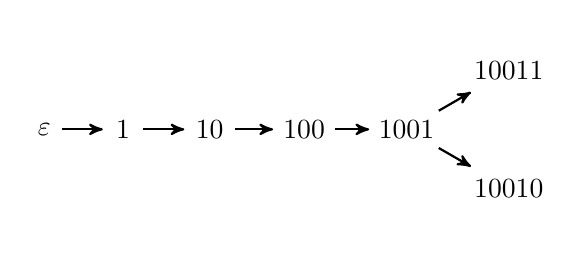
\begin{tikzpicture}[->,>=stealth',auto,thick, scale = 1.0,state/.style={circle,inner sep=2pt}]

    % The graph
	\node [state] at (0,0) (R) {$\varepsilon$};
	\node [state] at (1,0) (1) {$1$};
	\node [state] at (2.1,0) (10) {$10$};
	\node [state] at (3.3,0) (100) {$100$};
	\node [state] at (4.6,0) (1001) {$1001$};
	\node [state] at (5.9,0.75) (10011) {$10011$};
	\node [state] at (5.9,-0.75) (10010) {$10010$};	
	
	% Graph edges
	\path[->]
	(R) edge (1)
	(1) edge (10)
	(10) edge (100)
	(100) edge (1001)
	(1001) edge (10011)
	(1001) edge (10010)
	;  	
	


\end{tikzpicture} 
\end{center}
\caption{Although two paths are competing to become a blockchain, the blocks up to 1001 will contribute to the reward in each case. \label{fig-simple-fork}}
\end{figure}

In order to model the aforementioned scenario we need to introduce some notation.
Recall that a block $b$ is a string over the alphabet $\bP$, and we use notation $|b|$ for the length of $b$ as a string. Moreover, given blocks $b_1, b_2$, we use notation $b_1 \preceq b_2$ to indicate that $b_1$ is a prefix of $b_2$  when considered as strings. Then we define: 
\begin{eqnarray*}
\longest(q) & = & \{ b \in q \mid \text{for every } b' \in q: |b'| \leq |b|\}\\
\meet(q) & = & \{b \in q \mid \text{for every } b' \in \longest(q): b \preceq b'\}.
\end{eqnarray*}
Intuitively, $\longest(q)$ contains the leaves of all paths in the state $q$ that are currently competing for the blockchain, and $\meet(q)$ is the path from the genesis block to the last block for which all these paths agree on. For instance, if $q$ is the state from Figure~\ref{fig-simple-fork}, then we have that $\longest(q)=\{10011,10010\}$, and $\meet(q)=\{\varepsilon, 1, 10, 100, 1001\}$. Notice that $\meet(q)$ is well defined as $\preceq$ is a linear order on the finite and non-empty set $\{b \in q \mid \text{for every } b' \in \longest(q): b \preceq b'\}$. Also notice that $\meet(q)=\bchain(q)$, whenever $\bchain(q)$ is defined.


As mentioned before, the pay-off function will reward a player for the blocks in $\meet(q)$. Thus, to define the pay-off, we need to identify who is the owner of each one of these blocks, which is done by considering the function $\chi_p$, for each $p \in \bP$. More precisely, given $b \in \bB$, we have that:
\begin{eqnarray*}
\chi_p(b) & = & 
\begin{cases}
1 & \text{if } \owner(b) = p\\
0 & \text{otherwise}
\end{cases}
\end{eqnarray*}
We can finally define the payoff function we consider in this section, which we call \textbf{constant reward}. For a player $p$, we define it as 
\begin{eqnarray*}
r_p(q) & = & 
{\displaystyle c \cdot \sum_{b \in \meet(q)} \chi_p(b),}
\end{eqnarray*}
\martin{this reads odd since we do not use meet here. Is it correct?} \marcelo{I don't understand this comment, meet is used in the expression above.}
where $c$ is a positive real number. As mentioned above, this function is well defined since $\meet(q)$ always exists. Moreover, if $q$ has a blockchain, then we have that $\meet(q) = \bchain(q)$ and, hence, the pay-off function is defined for the blockchain of $q$.
% when the latter is defined for the state $q$.
%Here we use notation $b[i]$ for the $i$-th symbol in $b$, where $i \in \{1, \ldots, |b|\}$. 
% and $d \in \mathbb{N}$. Here the number $d$ is the amount of confirmations needed to spend the block (6 in the case of Bitcoin).
 
 \subsection{The default strategy maximizes the utility}

Let us start with analysing the most obvious strategy for all players: regardless of what everyone else does, keep mining on the blockchain, which is called the \emph{default} strategy.
More precisely, a player following the default strategy tries to mine upon the final block that appears in the blockchain of a state $q$. If the blockchain in $q$ does not exist, meaning that there are al least two longest paths from the genesis block, then the player tries to mine on the final block of one of these paths according to her rewards in them; she chooses the one that maximizes her reward, which in the case of constant reward means the path that contains the largest number of blocks belonging to her (if there is more than one of these paths, then between the final blocks of these paths she chooses the first according to a lexicographic order on the strings in $\{0, \ldots, m-1\}^*$). 
Notice that this is called the default strategy as it reflects the desired behaviour of the miners participating in the Bitcoin network.  For a player $p$, let us denote this strategy 
by $\df_p$, and consider the combined strategy $\cdf = (\df_0,\df_1,\dots,\df_{m-1})$. 
%Notice that under this strategy, each state $q$ consists of a single path from the genesis block $\varepsilon$ to the final block in $\bchain(q)$.

We can now easily calculate the utility of player $p$ under $\cdf$. Intuitively, a player $p$ will receive a fraction $h_p$ of the next block that is being placed in the blockchain, corresponding to her hash power. Therefore, at stage $i$ of the mining game, $i$ blocks will be placed in the blockchain defined by the game, and the expected amount of blocks owned by the player $p$ will be $h_p\cdot i$. This means that the total utility for player $p$ amounts to 
$$u_p(\cdf \mid \varepsilon) \ \ = \ \ (1 - \beta) \cdot h_p \cdot c\cdot \sum_{i=0}^{\infty}i \cdot \beta^{i} \ \ =  \ \ h_p\cdot c \cdot \frac{\beta}{(1-\beta)}.$$

%% Juan: I think it is way too nahive to put the analytical form of this
%$$u_p(\bs \mid q_0) = c\cdot h_p \cdot \sum_{i=0}^{\infty}i \cdot \beta^{i} \text{,}\ \ \ \ \text{ which evaluates to }\frac{c\cdot h_p}{(1-\beta)^2}.$$ %(recall that $q_0$ is the genesis block). 

The question then is: can any player do better? As we show in the following theorem, the answer is no as the default strategy maximizes the utility. 
\begin{mythm}\label{thm-conts_dom_str}
Let $p$ be a player, $\beta$ be a discount factor in $(0,1)$ and $u_p$ be the utility function defined in terms of $\beta$. Then for every combined strategy $\bs$:
\begin{eqnarray*}
u_p(\bs \mid \varepsilon) & \leq & u_p(\cdf \mid \varepsilon)
\end{eqnarray*}
\end{mythm} 

\begin{proof}
Let $\bs= (s_0, \ldots, s_{m-1})$ be an arbitrary combined strategy, and define $Q_\bs = \{q \in \bQ \mid \pr^\bs(q \mid \varepsilon) > 0\}$. Thus, $Q_\bs$ is the set of all states that can be reached from the genesis block using the combined strategy $\bs$. For example, we have that $Q_\cdf$ is the set of states $q$ such that $q$ consists of a single path from the genesis block to the final block in $\bchain(q)$.
Moreover, define a mapping $\sigma: Q_{\bs} \rightarrow 2^{Q_\cdf}$ as follows. Given two states $q_1, q_2$, we say that $q_2$ can be reached from $q_1$ in one step if $q_2 = q_1 \cup \{ b \cdot p' \}$, where $b \in \bB$, $p' \in \bP$ and $b \cdot p' \not\in q_1$ (recall that $\bB = \{0, \ldots, m-1\}^*$ and $\bP = \{0, \ldots, m-1\}$); that is, we have that $q_2$ can be reached from $q_1$ in one step  if $q_2$ is the result of applying action $\mine(p', b, q_1)$, where $\mine(p', b, q_1)$ is a valid action for player $p'$. 
Then for each state $q \in Q_{\bs}$, consider all distinct sequences $\rho = q_0,\dots,q_n$ such that $q_{i+1}$ can be reached from 
$q_i$ in one step ($i \in \{1, \ldots, n-1\}$), $q_0 = \varepsilon$ and $q_n = q$. To each such a sequence $\rho = q_0,\dots,q_n$, associate a block $b_\rho$ of length $n$ as follows.
% in $\{0,1\}^*$ 
For every $i \in \{1, \ldots, n\}$, if for a player $p' \in \bP$, it holds that $s_{p'}(q_{i-1}) = a_{p'}$ and $q_{i} = a_{p'}(q_{i-1})$, then $i$-th symbol of $b$ is $p'$. Notice that the $i$-th symbol of $b_\rho$ is well defined as $q \in Q_\bs$ and the sets of actions for two distinct players are disjoint.
%Notice that if  $b_i = 1$, then $q_{i} = a_1(q_{i-1})$ with $a_1 = \df_1(q_{i-1})$. 
Finally, define $\sigma(q)$ as the set of all states $q' \in Q_\cdf$ consisting of a single path whose final block is a block $b_\rho$ associated to a sequence $\rho$ for $q$; formally, we have that:
\begin{multline*}
\sigma(q) \ = \ \big\{q' \in Q_\cdf \mid \text{there exists a sequence } \rho \text{ for } q\\ \text{ such that } q' = \{ b \in \bB \mid b \preceq b_\rho \}\big\}.
\end{multline*}
%for which there exist a sequence $\rho$ and a corresponding block $b_\rho$ such that $q' = \{ b \in \bB \mid b \preceq b_\rho \}$
%and where 
%$q^*$ is the smallest prefix closed set of strings containing $w$. 
%
In this proof, we need the following property of the mapping $\sigma$.

\begin{myclaim}
\label{claim-nonempty-inter-gen}
For every pair of distinct states $q,q'$ in $Q_{\bs}$, the sets $\sigma(q)$ and $\sigma(q')$ are disjoint. 
\end{myclaim}

\begin{proof}
For the sake of contradiction, assume that
%Assume for contradiction two different  states 
$q,q'$ are two distinct states in $Q_{\bs}$ such that both $\sigma(q)$ and $\sigma(q')$ contain a state $q^* \in Q_\cdf$. By definition of $Q_\cdf$, there exists a block 
%$w$ 
$b^*$ such that $q^* = \{b \in \bB \mid b \preceq b^*\}$.
% is the closure (over prefixes) of $w$. 
By definition of mapping $\sigma$, there exist a sequence $\rho = q_0,\dots,q_n$ for $q$ and a sequence $\rho' = q_0',\dots,q_n'$ for $q'$ such that $b^* = b_\rho$ and $b^* = b_{\rho'}$. If 
$\rho = \rho'$, then $q = q'$ as $q = q_n$ and $q' = q'_n$. Hence, we have that $\rho \neq \rho'$.
%, so $\rho$ must be different from $\rho'$. 
Let $i$ be the first position where $\rho$ and $\rho'$ differ,
%are different, 
so that 
sequences $q_0,\dots,q_{i-1}$ and $q_0,\dots,q'_{i-1}$ are the same and $q_i \neq q_i'$ (notice that $i \in \{1, \ldots, n\}$ since $q_0 = q'_0 = \varepsilon$).
%except for the last state. 
Then both $q_i$ and $q_i'$ are reachable from $q_{i-1}$ in one step. Therefore, it follows that 
%by the construction of our game 
$q_i = a_{p_1}(q_{i-1})$ and $q'_i = a_{p_2}(q_{i-1})$, where $a_{p_1} = s_{p_1}(q_{i-1})$, $a_{p_2} = s_{p_2}(q_{i-1})$ and $p_1 \neq p_2$. Hence, we have that the symbols in the $i$-th positions of $b_\rho$ and $b_{\rho'}$ are different, from which we conclude that $b_\rho \neq b_{\rho'}$, and reach a contradiction since $b^* = b_\rho$ and $b^* = b_{\rho'}$.
%is different from the symbol in the $
%the word generated from $\pi$ and $\pi'$ is not the same. 
\end{proof}
Recall that the utility of player $p$ using combined strategy $\cdf$ 
%at the genesis tree 
is defined as:
\begin{eqnarray*}
u_p(\cdf \mid \varepsilon) & = & \sum_{q \in \bQ} \beta^{|q|} \cdot  r_p(q) \cdot \pr^{\cdf}(q \mid \varepsilon).
\end{eqnarray*}
If we choose to sum only over the states in the images under $\sigma$ of the states of $Q_\bs$, then by Claim \ref{claim-nonempty-inter-gen} we have that:
\begin{eqnarray*}
u_p(\cdf \mid \varepsilon) & \geq & \sum_{q \in \sigma(q^*) \,:\, q^* \in Q_{\bs}} \beta^{|q|} \cdot  r_p(q) \cdot \pr^{\cdf}(q \mid \varepsilon).
\end{eqnarray*}
%because Claim \ref{claim-nonempty-inter} guarantees that we are not summing each state in $Q_\df$ more than once. %We 
Rearranging the term in the right-hand side, we obtain:
\begin{eqnarray*}
u_p(\cdf \mid \varepsilon) & \geq &\sum_{q^* \in Q_{\bs}}   \sum_{q \in \sigma(q^*)} \beta^{|q|} \cdot  r_p(q) \cdot \pr^{\cdf}(q \mid \varepsilon).
\end{eqnarray*}
For each state $q^* \in Q_{\bs}$, notice that if $q \in \sigma(q^*)$, then $|q| = |q^*|$ and the number blocks owned by $p$ in $q$ is the same as the number of blocks owned by $p$ in $q^*$. Thus, we have that $r_p(q) \geq r_p(q^*)$ since $q \in Q_{\cdf}$ and, therefore, every block owned by $p$ in $q$ is in $\bchain(q)$ and $\bchain(q) = \meet(q)$.
        Notice that it could be the case that $r_p(q) > r_p(q^*)$, as some blocks owned by $p$ in $q^*$  may not be in $\meet(q^*)$. We conclude that:
\begin{align*}
\sum_{q \in \sigma(q^*)} \beta^{|q|} \cdot  r_p(q) \, \cdot \, & \pr^{\cdf}(q \mid \varepsilon) \geq \\
&\sum_{q \in \sigma(q^*)} \beta^{|q^*|} \cdot  r_p(q^*) \cdot \pr^{\cdf}(q \mid \varepsilon) = \\
&\beta^{|q^*|} \cdot  r_p(q^*) \sum_{q \in \sigma(q^*)}  \pr^{\cdf}(q \mid \varepsilon).
\end{align*}
% because $|q| = |q^*|$ and 
%$q$ and $q^*$ have the same number of blocks owned by $0$. 
Moreover, by definition of $\pr^{\cdf}$ and $\pr^\bs$, we have that:
\begin{eqnarray*}
\sum_{q \in \sigma(q^*)}  \pr^{\cdf}(q \mid \varepsilon) & = & \pr^{\bs}(q^* \mid \varepsilon).
\end{eqnarray*}
Combining the previous results and considering that $\pr^{\bs}(q^* \mid \varepsilon) = 0$ for every $q^* \in \bQ \smallsetminus Q_{\bs}$, we conclude that: 
\begin{eqnarray*}
u_p(\cdf \mid \varepsilon) & \geq & \sum_{q^* \in Q_\bs} \bigg(\beta^{|q^*|} \cdot  r_p(q^*) \sum_{q \in \sigma(q^*)}  \pr^{\cdf}(q \mid \varepsilon)\bigg)\\
& = & \sum_{q^* \in Q_\bs} \beta^{|q^*|} \cdot  r_p(q^*) \cdot \pr^{\bs}(q^* \mid \varepsilon)\\
& = & \sum_{q^* \in \bQ} \beta^{|q^*|} \cdot  r_p(q^*) \cdot \pr^{\bs}(q^* \mid \varepsilon)\\
& = & u_p(\bs \mid \varepsilon), 
\end{eqnarray*}
which was to be shown.
\end{proof}
As a corollary of Theorem \ref{thm-conts_dom_str}, we obtain that:
\begin{mycor}\label{cor-conts_equlibria}
For every $\beta \in (0,1)$, the strategy $\cdf$ is a $\beta$-discounted stationary equilibrium.
\end{mycor} 
While constant-block reward do not faithfully model reality, since in the Bitcoin protocol the reward decreases every approximately four years, we would like to argue why Theorem \ref{thm-conts_dom_str} could serve as a recommendation on how to enforce good behaviour on miners at the moment block rewards become insignificant. More precisely, if block rewards are negligible, the transaction fees will dictate the miners' pay-off, so the protocol could place a (constant) total fee limit on newly created blocks. \marcelo{We need to argue why it is reasonable to impose a (constant) total fee limit in this scenario.} Assuming that the volume of transactions is high, the blocks would regularly achieve the maximal reward, thus making the block reward constant. Theorem  \ref{thm-conts_dom_str} then tells the miners that their best strategy is to mine on top of the existing blockchain, as this will maximize their utility in the long run.
\marcelo{Same comment as at the beginning of this section, we need to change this paragraph considering the more general view of our framework for cryptocurrencies.}

% \subsection{The default strategy is an equilibrium}
%
%Let us start with analysing the most obvious strategies for all players: regardless of what everyone else does, keep mining on the blockchain. We call this 
%the \emph{default} strategy, as it reflects the desired behaviour of the miners participating in the Bitcoin network. 
%For a player $p$, let us denote this strategy 
%by $\df_p$, and consider the combined strategy $\cdf = (\df_0,\df_1,\dots,\df_{m-1})$. Notice that under this strategy, each state $q$ consists of a single path from the genesis block $\varepsilon$ to the final block in $\bchain(q)$.
%
%We can now easily calculate the utility of player $p$ under $\cdf$. Intuitively, a player $p$ will receive a fraction $h_p$ of the next block that is being placed in the blockchain, corresponding to her hash power. Therefore, at stage $i$ of the mining game, $i$ blocks will be placed in the blockchain defined by the game, and the expected amount of blocks owned by the player $p$ will be $h_p\cdot i$. This means that the total utility for player $p$ amounts to 
%$$u_p(\cdf \mid \varepsilon) \ \ = \ \ h_p \cdot c\cdot \sum_{i=0}^{\infty}i \cdot \beta^{i} \ \ =  \ \ h_p\cdot c \cdot \frac{\beta}{(1-\beta)^2}.$$
%
%%% Juan: I think it is way too nahive to put the analytical form of this
%%$$u_p(\bs \mid q_0) = c\cdot h_p \cdot \sum_{i=0}^{\infty}i \cdot \beta^{i} \text{,}\ \ \ \ \text{ which evaluates to }\frac{c\cdot h_p}{(1-\beta)^2}.$$ %(recall that $q_0$ is the genesis block). 
%
%The question then is: can any player do better? As we show, the answer is no if we assume that the rest of the players behave according to $\cdf$. More precisely, we have the following result. 
%
%\begin{mythm}\label{thm-conts_equlibria}
%For every $\beta \in [0,1)$, the strategy $\cdf$ is a $\beta$-discounted stationary equilibrium.
%\end{mythm} 
%
%\begin{proof}
%Let $p \in \bP$ be a player and $s_p$ be an arbitrary strategy for~$p$. We need to show that the utility of $(\cdf_{-p},s_p)$ is not higher than the utility of $\cdf$ for player $p$, that is, we need to show that $u_p((\cdf_{-p},s_p) \mid \varepsilon) \leq u_p(\cdf \mid \varepsilon)$. 
%
%First, observe that it is enough to consider a two-player game, as all the players except $p$ can be merged into a single player whose hash power is the sum of the hash power 
%of each player $p' \neq p$. 
%%of the aggregated players. 
%Thus, we consider $\bP = \{0,1\}$, and for readability we assume  that $p = 0$ (the other case being symmetric). Notice that under these assumptions, it holds that $(\cdf_{-p},s_p) = (s_0, \df_1)$. 
%
%For a combined strategy $\bs$, let $Q_\bs = \{q \in \bQ \mid \pr^\bs(q \mid \varepsilon) > 0\}$. Thus, $Q_\bs$ is the set of all states that can be reached from the genesis block using the combined strategy $\bs$. For example, we have that $Q_\cdf$ is the set of states $q$ such that $q$ consists of a single path from the genesis block to the final block in $\bchain(q)$.
%Moreover, define a mapping $\sigma: Q_{(s_0,\df_1)} \rightarrow 2^{Q_\cdf}$ as follows. Given two states $q_1, q_2$, we say that $q_2$ can be reached from $q_1$ in one step if $q_2 = q_1 \cup \{ b \cdot p' \}$, where $b \in \{0,1\}^*$, $p' \in \bP$ and $b \cdot p' \not\in q_1$; that is, we have that $q_2$ can be reached from $q_1$ in one step  if $q_2$ is the result of applying action $\mine(p', b, q_1)$, where $\mine(p', b, q_1)$ is a valid action for player $p'$. 
%Then for each state $q \in Q_{(s_0,\df_1)}$, enumerate all distinct sequences $\pi = q_0,\dots,q_n$ such that $q_{i+1}$ can be reached from 
%$q_i$ in one step ($i \in \{1, \ldots, n-1\}$) , $q_0 = \varepsilon$ and $q_n = q$. To each such sequence $\pi$, associate a block $b_\pi = b_1 \cdots b_n$
%% in $\{0,1\}^*$ 
%such that:
%\begin{eqnarray*}
%b_i & = &
%\begin{cases}
%0 & \text{if } q_{i} = a_0(q_{i-1}), \text{ where } a_0 = s_0(q_{i-1}) \\
%1 & \text{if } q_{i} = a_1(q_{i-1}), \text{ where } a_1 = \df_1(q_{i-1})
%\end{cases}
%\end{eqnarray*}
%%Notice that if  $b_i = 1$, then $q_{i} = a_1(q_{i-1})$ with $a_1 = \df_1(q_{i-1})$. 
%Finally, define $\sigma(q)$ as the set of all states $q' \in Q_\cdf$ for which there exist a sequence $\pi$ and a corresponding block $b_\pi$ such that $q' = \{ b \in \{0,1\}^* \mid b \preceq b_\pi \}$.
%%and where 
%%$q^*$ is the smallest prefix closed set of strings containing $w$. 
%
%In this proof, we need the following property of the mapping $\sigma$.
%
%\begin{myclaim}
%\label{claim-nonempty-inter}
%For every pair of distinct states $q,q'$ in $Q_{(s_0,\df_1)}$, the sets $\sigma(q)$ and $\sigma(q')$ are disjoint. 
%\end{myclaim}
%
%\begin{proof}
%For the sake of contradiction, assume that
%%Assume for contradiction two different  states 
%$q,q'$ are two distinct states in $Q_{(s_0,\df_1)}$ such that both $\sigma(q)$ and $\sigma(q')$ contain a state $q^* \in Q_\cdf$. By definition of $Q_\cdf$, there is a block 
%%$w$ 
%$b^*$ such that $q^* = \{b \in \{0,1\}^* \mid b \preceq b^*\}$.
%% is the closure (over prefixes) of $w$. 
%By definition of mapping $\sigma$, there exist a sequence $\pi = q_0,\dots,q_n$ for $q$ and a sequence $\pi' = q_0',\dots,q_n'$ for $q'$ such that $b^* = b_\pi$ and $b^* = b_{\pi'}$. If 
%$\pi = \pi'$, then $q = q'$ as $q = q_n$ and $q' = q'_n$. Hence, we have that $\pi \neq \pi'$.
%%, so $\pi$ must be different from $\pi'$. 
%Let $i$ be the first position where $\pi$ and $\pi'$ differ,
%%are different, 
%so that 
%sequences $q_0,\dots,q_{i-1}$ and $q_0,\dots,q'_{i-1}$ are the same and $q_i \neq q_i'$ (notice that $i \in \{1, \ldots, n\}$ since $q_0 = q'_0 = \varepsilon$).
%%except for the last state. 
%Then both $q_i$ and $q_i'$ are reachable from $q_{i-1}$ in one step. Therefore, it follows that 
%%by the construction of our game 
%one of $q_i$, $q_i'$ is the result of applying action $s_0(q_{i-1})$  and the other is the result of applying $\df_1(q_{i-1})$, which implies that the symbols in the $i$-th positions of $b_\pi$ and $b_{\pi'}$ are different. Hence, we conclude that $b_\pi \neq b_{\pi'}$, which leads to a contradiction since $b^* = b_\pi$ and $b^* = b_{\pi'}$.
%%is different from the symbol in the $
%%the word generated from $\pi$ and $\pi'$ is not the same. 
%\end{proof}
%Recall that the utility of player $0$ using combined strategy $\cdf$ 
%%at the genesis tree 
%is defined as:
%\begin{eqnarray*}
%u_0(\cdf \mid \varepsilon) & = & \sum_{q \in \bQ} \beta^{|q|} \cdot  r_0(q) \cdot \pr^{\cdf}(q \mid \varepsilon).
%\end{eqnarray*}
%If we choose to sum only over the states in the images under $\sigma$ of the states of $Q_{(s_0,\df_1)}$, then by Claim \ref{claim-nonempty-inter} we have that:
%\begin{eqnarray*}
%u_0(\cdf \mid \varepsilon) & \geq & \sum_{q \in \sigma(q^*) \,:\, q^* \in Q_{(s_0,\df_1)}} \beta^{|q|} \cdot  r_0(q) \cdot \pr^{\cdf}(q \mid \varepsilon).
%\end{eqnarray*}
%%because Claim \ref{claim-nonempty-inter} guarantees that we are not summing each state in $Q_\df$ more than once. %We 
%Rearranging the term in the right-hand side, we obtain:
%\begin{eqnarray*}
%u_0(\cdf \mid \varepsilon) & \geq &\sum_{q^* \in Q_{(s_0,\df_1)}}   \sum_{q \in \sigma(q^*)} \beta^{|q|} \cdot  r_0(q) \cdot \pr^{\cdf}(q \mid \varepsilon).
%\end{eqnarray*}
%For each state $q^* \in Q_{(s_0,\df_1)}$, notice that:
%\begin{align*}
%\sum_{q \in \sigma(q^*)} \beta^{|q|} \cdot  r_0(q) \, \cdot \, & \pr^{\df}(q \mid \varepsilon) \geq \\
%&\sum_{q \in \sigma(q^*)} \beta^{|q^*|} \cdot  r_0(q^*) \cdot \pr^{\df}(q \mid \varepsilon) = \\
%&\beta^{|q^*|} \cdot  r_0(q^*) \sum_{q \in \sigma(q^*)}  \pr^{\df}(q \mid \varepsilon),
%\end{align*}
% because $|q| = |q^*|$ and 
%$q$ and $q^*$ have the same number of blocks owned by $0$. By definition, we also have that:
%\begin{eqnarray*}
%\sum_{q \in \sigma(q^*)}  \pr^{\cdf}(q \mid \varepsilon) & = & \pr^{(s_0,\df_1)}(q^* \mid \varepsilon).
%\end{eqnarray*}
%Summing up and rearranging, we conclude that: 
%\begin{eqnarray*}
%u_0(\cdf \mid \varepsilon) & \geq & \sum_{q^* \in Q_{(s_0,\df_1)}}  \beta^{|q^*|} \cdot  r_0(q^*) \cdot \pr^{(s_0,\df_1)}(q^* \mid \varepsilon)\\
%& = & u_0((s_0,\df_1) \mid \varepsilon), 
%\end{eqnarray*}
%which was to be shown.
%\end{proof}
%
%
%While constant block rewards do not faithfully model reality, since in the Bitcoin protocol the reward decreases every 200.000 blocks or so, we would like to argue why Theorem \ref{thm-conts_equlibria} could serve as a good recommendation on how to enforce good behaviour on miners at the moment block rewards become insignificant. More precisely, if block rewards are negligible, the transaction fees will dictate the miners' pay-off, so the protocol could place a (constant) total fee limit on newly created blocks. Assuming that the volume of transactions is high, the blocks would regularly achieve the maximal reward, thus making the block reward constant. Theorem \ref{thm-conts_equlibria} then tells the miners that their best strategy is to mine on top of the existing blockchain, as this will maximize their utility in the long run.


%The remainder of this section is devoted to explaining the proof of  Theorem \ref{thm-conts_equlibria}.

%
%\subsection{Greedy strategies and proof of Theorem \ref{thm-conts_equlibria}} 
%
%We begin by showing that $\df$ is an equilibrium when we slightly restrict the space of strategies that the player use, and concentrate on the so called {\em greedy} strategies. Intuitively, under greedy strategies, the players refrain from forking on top of blocks that appear before their latest block when there is no blockchain, or their latest block in the blockchain, when the latter is defined. Greedy strategies can be formally defined as follows. 
%Given a player $p \in \bP$ and a state $q \in \bQ$, let:
%\begin{multline*}
%\longest(q,p) \ = \ \{ b \in q \mid (b = \varepsilon \text{ or } \owner(b) = p),\\
%\text{ and for every } b' \in q \text{ such that } \owner(b') = p : |b'| \leq |b|\}
%\end{multline*}
%Notice that $\varepsilon \in \longest(p,q)$ if and only if there is no $b \in q$ such that $\owner(b) = p$. Moreover, define $\length(q,p)$ as the length of an arbitrary string in $\longest(q,p)$ (all of them have the same length).
%\begin{mydef}\label{def-greedy}
%Given $p \in \bP$, $b \in \bB$ and $q \in \bQ$,  an action $\mine(p,b,q)$ is {\em greedy} if $\mine(p,b,q)$ is a valid action and $\length(q,p) \leq |b|$.
%
%Moreover, a combined strategy $\bs = (s_0, s_1, \ldots, s_{m-1})$ is {\em greedy} if for every $p \in \bP$ and  $q \in \bQ$ such that $\pr^{\bs}(q \mid \varepsilon) > 0$, it holds that $s_p(q)$ is a greedy action.
%\end{mydef}
%
%For now, we only consider greedy strategies. 
%%
%%Under greedy strategies, players refrain to fork on top of blocks that appear before their latest block, or their latest block in the blockchain. 
%The consequence of this is that every state in an $m$-player game under greedy strategies cannot have more than $m$ paths contesting for the blockchain. More precisely:% (see Lemma \ref{lem-length-greedy} in Appendix \ref{sec-char-states-greedy}). %This is captured b the following technical lemma: 
%\begin{mylem}\label{lem-length-greedy}
%Let $\bs$ be a greedy strategy. Then for every $q \in \bQ$ such that $\pr^{\bs}(q \mid \varepsilon) > 0$, the following conditions hold:
%\begin{enumerate}
%\item For every $p \in \bP$ $:$ $|\longest(q,p)| = 1$ 
%
%\item There exists $I \subseteq \bP$ such that$:$
%\begin{eqnarray}\label{eq-max-set}
%\longest(q) & = & \bigcup_{p \in I} \longest(q,p).
%\end{eqnarray}
%Moreover, if $q \neq \{\varepsilon\}$, then there exists a unique $I \subseteq \longest(q,p)$ such that \eqref{eq-max-set} holds.
%\end{enumerate}
%\end{mylem}
%
%The key property of greedy strategies needed to show that $\df$ is an equilibrium, is the fact that if two strategies are optimal for a player $p$, then they can not differentiate two states $q$ and $q'$ in which the subtree rooted at $\longest(q,p)$ and $\longest(q',p)$, respectively, are isomorphic. A strategy $s$ for a player $p$ is called a {\em basic strategy}, if $s(q)=s(q')$, whenever the subtree of $q$ rooted at $\longest(q,p)$ is isomorphic to the subtree of $q'$ rooted at $\longest(q',p)$. We can show that for greedy strategies the following holds:
%
%\begin{mylem}
%\label{lem-meet}
%Consider a game with $m$ players and let $s_p$ be a greedy strategy for player $p$. Then there is a basic strategy $s'_p$ such that $u_p((s_{-p},s'_p) \mid \varepsilon) \geq u_p((s_{-p},s_p) \mid \varepsilon)$ for any set $s_{-p}$ of basic greedy strategies.  
%\end{mylem}
%
%
%With this lemma at hand, we can now show that $\df$ is indeed a stationary equilibrium when we are considering only greedy strategies.
%
%\begin{mythm}%\label{thm-conts_equlibria}
%For any $0 \leq \beta \leq 1$, the strategy $\df$ is a $\beta$-discounted stationary equilibrium under greedy strategies. 
%\end{mythm} 
%
%\etienne{In order for the theorem to be true we have to considere stable DF strategy and not whatever df strategy. I think the easiest way to add this constraint without too much work is directly in the definition of greedy strategy ! A greedy action is ok, but to be a greedy strategy you also have to be stable.}
%EXPLAIN SOME BASIC IDEAS BEHIND THE PROOF.
%
%Having established that $\df$ is an equilibrium under greedy strategies, we will now show that this restriction is not necessary, as any non greedy strategy can be replaced by a greedy one in an equilibrium. That is, we can show the following:
%
%LEMMA REUTTER-TOUSSAINT
%
%EXPLAIN WHY THE LEMMA SHOW THAT DF IS GREAT.
%
%
%%We conclude this section by some remarks on the potential significance of Theorem \ref{thm-conts_equlibria}. As we have already mentioned, constant block rewards do not faithfully model reality, since in the Bitcoin protocol the reward decreases every 200.000 blocks or so. However, we would like to argue that Theorem \ref{thm-conts_equlibria} can serve as a good recommendation on how to enforce good behaviour on miners (assuming they will use the utility function as an indicator of their monetary gain), at the moment block rewards become insignificant. More precisely, if block rewards are insignificant, and the transaction fees dictate the miners' pay-off, the protocol could place a (constant) fee limit on newly created blocks. Assuming that the volume of transactions is high, the blocks would regularly achieve the maximal reward, thus making the block reward constant. Theorem \ref{thm-conts_equlibria} then tells the miners that their best strategy is to mine on top of the existing blockchain, as this will maximize their utility in the long run.
%
%
%%We already mentioned that constant block rewards do not faithfully model reality, since in the Bitcoin protocol the reward decreases every 200.000 blocks or so. However, we would like to argue that Theorem \ref{thm-conts_equlibria} can serve as a good recommendation on how to enforce good behaviour on miners (assuming they will use the utility function as an indicator of their monetary gain), at the moment block rewards become insignificant. More precisely, if block rewards are insignificant, and the transaction fees dictate the miners' pay-off, the protocol could place a (constant) fee limit on newly created blocks. Assuming that the volume of transactions is high, the blocks would regularly achieve the maximal reward, thus making the block reward constant. Theorem \ref{thm-conts_equlibria} then tells the miners that their best strategy is to mine on top of the existing blockchain, as this will maximize their utility in the long run.

	%!TEX root = focs.tex

\section{Decreasing Payoff}
\label{sec-dec}

%While interesting, readers could argue that the payoff function considered before is not completely modelling bitcoin, because in bitcoin 
%the reward given for mining blocks is reduced by half every 200.000 blocks or so. Thus the natural question, do the results above continue to hold under these 
%circumstances? Our answer is a resounding no, and now forking can be a valid strategy depending on the hash power of a player (and the other parameters of the game). 

While interesting, readers could argue that the constant reward considered in the previous section is not a faithful model of the Bitcoin protocol, where the reward diminishes over time. Thus, it is natural to ask whether  mining on top of the existing blockchain continues to be an  optimal strategy under these 
circumstances? Our answer is a resounding no, and as we show in this section, when the reward decreases over time, forking can be a valid strategy depending on the hash power of a player (and the other parameters of the game). 

For simplicity, we model the diminishing rewards in bitcoin as a constant factor that is lowered after every new block in the blockchain. That is, in this section 
we use the following pay-off function $r_p$ for all players $p \in \bP$, denoted as the \textbf{$\alpha$-discounted reward}: 
\begin{eqnarray*}
r_p(q) & = & 
{\displaystyle c \cdot \sum_{i=1}^{|\meet(q)|} \alpha^i \cdot \chi_p(\meet(q),i)} \end{eqnarray*}
where $c$ is a positive real number and $\alpha \in (0,1]$.

\medskip

(say that the approach we use is the same as above: we consider a two player game and group a bunch of well behaved players 
into a single player. Also state that the subtree lemma holds also for this payoff)

\subsection{When is forking a good strategy}
\label{sec-forkingstrategies}
(probably say this is a very interesting open question in the literature). 

In order to understand when forking could be a good strategy, let us consider again the two player game in which player $p$ has just mined a block in the blockchain. 
Now, if player $(1-p)$ wins the next block, player $p$ faces two different options. She could continue mining on the blockchain, playing according to $\df$, or she 
could fork, mining instead upon her previously won block. Which strategy is better? To answer this question, we need to calculate the utility in both cases. For 
simplicity, and without loss of generality (due to Lemma [?]), we will focus on this question when the game is just starting, in the genesis block, and we will assume that 
player $p$ resumes the default strategy (mining upon the blockchain) as soon as she wins the fork. 

More precisely, we will calculate the utility of the combined strategy $(\df_{1-p},\fg_p)$, where $\fg_p$ is the \textbf{Fork on the genesis} 
strategy, defined as follows for a state $q \in \bQ$:
%\begin{eqnarray*}
%\fg_p(q) & = &
%\begin{cases}
%\mine(p,\varepsilon,q) & \text{if } p \not\in q\\
%\mine(p,\bchain(q),q) &  \text{if } \bchain(q) \text{ is defined and } p \preceq \bchain(q)\\
%\mine(p,b,q) &  \text{if } \bchain(q) \text{ is defined},\  p \in q,\ p \not\preceq \bchain(q)
%\text{ and}\\
%&  \hspace{50pt} {\displaystyle b = \max_{\preceq} \, \{ b' \in q \mid \longest(q,p) \preceq b'\}}\\
%\mine(p,\longest(q,p),q) &  \text{if } \bchain(q) \text{ is not defined},\ p \in q \text{ and}\\
%& \hspace{50pt} p \not\preceq \longest(q,1-p)\\
%\mine(p,\longest(q,p),q) &  \text{if } \bchain(q) \text{ is not defined},\ p \preceq \longest(q,1-p) \text{ and}\\
%& \hspace{50pt} r_p(\longest(q,p)) \geq r_p(\longest(q,1-p))\\
%\mine(p,\longest(q,1-p),q) &  \text{if } \bchain(q) \text{ is not defined},\  p \preceq \longest(q,1-p) \text{ and}\\
%& \hspace{50pt} r_p(\longest(q,p)) < r_p(\longest(q,1-p))
%\end{cases}
%\end{eqnarray*}
\begin{eqnarray*}
\fg_p(q) & = &
\begin{cases}
\mine(p,\varepsilon,q) & \text{if } p \not\in q\\
\df_p(q) & \text{if } \bchain(q) \text{ is defined and } p \preceq \bchain(q) \text{ or}\\
& \hspace{70pt} \bchain(q) \text{ is not defined and } p \preceq \longest(q,1-p)\\
\mine(p,b,q) &  \text{otherwise, where } {\displaystyle b = \max_{\preceq} \, \{ b' \in q \mid \longest(q,p) \preceq b'\}}
\end{cases}
\end{eqnarray*}
Notice that in this definition, the set $\{ b' \in q \mid \longest(q,p) \preceq b'\}$ has a maximum element under the partial order $\preceq$ as all the elements in this set are of the form $\longest(q,p) \cdot (1-p)^\ell$ with $\ell \geq 0$.

(show how to compute the utility, put graphics, compare. 

\subsection{More complicated cases}

Speak of $m$-fork as a refinement of the previous strateegy, put give-up time if we have it as well. Graphics, compare, etc. 

\subsection{Stationary equilibrium}

Need to fill this up! 

	
	%\section{old stuff}

\medskip
\noindent
\textbf{Block chain game}

\begin{mydef}
A block-chain game is a tuple $(G,V,\preceq_{G,V},P,\mathcal K,D)$ where $V$ is a validation rule, $G$ a list of genesis blocks, $\preceq_{G,V}$ a block chain protocol over $LOG_{G,V}$, $P$ a set of player, $\mathcal K$ a function which map each player of $P$ to a knowledge tree and $D : P \rightarrow [0, 1] $ such that $$\sum_{p\in P} D(p) = 1 \lor \sum_{p\in P} D(p) = 0$$ 
\end{mydef}
$D(p)$ represents the probability, that a player $p$, has to be the first to discover a list $L \in LOG_{G,V}$ such that for all $L'$ block chain of $\mathcal K (p)$ with respect to $\preceq_{G,V}(t)$, $L \neq L'$ and $L \preceq_{G,V,t} L'$

\begin{mydef}
	A block-chain game $(G,V,\preceq_{G,V},P,\mathcal K,D)$ is said to be alive if $$\sum_{p\in P} D(p) = 1$$
\end{mydef}

\medskip
\noindent
\textbf{Strategies for discovery}

\begin{mydef}
	A \emph{strategy} is a partial function $S: \B \times \mathbb{N} \rightarrow [0,1]$ that 
	satisfies $S(B,i) \leq S(B,j)$ for all $i \leq j$. That is, $S$ assigns 
	to each block $B$ and number $i$ a probability $S(B,i)$ that is not decreasing on $i$. 
\end{mydef}

Intuitively, a strategy assigns to a time $i$ a probability that a certain block is discovered amongst the 
$i$ next blocks that are discovered. 

\begin{mydef}
	Given a genesis $G$ and a validation function $V$, 
	A Knowledge representation for $G$ and $V$ is a pair $(K,S)$, where $K$ is a knowledge tree and 
	$S$ is a strategy with preimage $\{B \in \B \mid B \notin K\} \times \mathbb N$. 
\end{mydef}

Let $\mathcal K$ be a set $\{(K_1,S_1),\dots,(K_n,S_n)\}$ of knowledge trees. 
We say that $LOG_{G,V}$ is alive with respect to $\mathcal K$ if there is an $(K_\ell,S_\ell)$ with $1 \leq \ell \leq n$ 
and a block $B$ not in $K_\ell$ such that 
$$\lim\limits_{\delta\rightarrow +\infty}S_\ell(B,\delta) = 1$$

$LOG_{G,V}$ is alive with respect to $\mathcal K$ and a protocol $\preceq_{G,V}$ on a time $t$
if there is an $(K_\ell,S_\ell)$ with $1 \leq \ell \leq n$ 
and a block $B \in V(BC_t)$ such that 
$$\lim\limits_{\delta\rightarrow +\infty}S_\ell(B,\delta) = 1, $$
where $BC_t$ is a blockchain of $K_\ell$ with respect to $\preceq_{G,V}$ in $t$.

\begin{mydef}
Let $P$ be a set of players and $K_T$ a function :
$$K_{T} : P \times \llbracket 0;T \rrbracket \times \mathbb{N} \rightarrow \fset(\B \times [0;1])$$ 
Then $(P,K_{T})$ is a valid knowledge representation if :

\begin{eqnarray*}
&\forall p \in P,\forall t\in \llbracket 0;T \rrbracket, (b,\alpha) \in K_{T}(t,0,p) \implies \alpha = 1 \lor \alpha = 0\\
&\forall p \in P,\forall t,t'\in \llbracket 0;T \rrbracket, t' \geq t, \forall b \in \B,  (b,1) \in K_{T}(t,0,p) \implies (b,1) \in K(t',0,p)  \\
&\forall p \in P,\forall t\in \llbracket 0;T \rrbracket, \forall \delta \in \mathbb{N}, \forall b \in \B,  (b,1) \in K_{T}(t,0,p) \implies (b,1) \in K(t,\delta,p) \\
&\forall p \in P,\forall t\in \llbracket 0;T \rrbracket, \forall \delta,\delta' \in \mathbb{N}, \delta' \geq \delta \implies \forall (b,\alpha) \in K_{T}(p,t,\delta), \exists (b,\alpha') \in K_{T}(p,t,\delta'), \alpha'\geq \alpha\\
\end{eqnarray*}
\end{mydef}

\begin{mynota}
	$\forall p \in P, \forall t\in \llbracket 0;T \rrbracket$ we denote $$K_{T}(p,t)=\{b | (b,1) \in K_{T}(p,t,0)\}$$
\end{mynota}

\begin{mydef}
	Let $T,T' \in \mathbb{N}$ such that $T>T'$ we say that $K'_{T'}$ extend $K_{T}$ if $$\forall p, K_{T}(p,T) = K'_{T'}(p,T)$$
\end{mydef}

\begin{mydef}
	Let $\preceq_{G,V,t}$ be  a total preorder over $LOG_{G,V}$:
\begin{eqnarray*}		
	&\forall L_1, L_2, L_3 \in LOG_{G,V}, L_1 \preceq_{G,V,t} L_2 \land L_2 \preceq_{G,V,t} L_3 \implies L_1 \preceq_{G,V,t} L_3  \\
	&\forall L_1, L_2 \in LOG_{G,V}, L_1 \preceq_{G,V,t} L_2 \lor L_2 \preceq_{G,V,t} L_1 
\end{eqnarray*}
	A block chain protocol over $LOG_{G,V}$ is a function noted $\preceq_{G,V}$ such that: $$ \forall t \in \mathbb{N}, \preceq_{G,V}(t) =  \preceq_{G,V,t}$$ where $\preceq_{G,V,t}$ is a total preorder over $LOG_{G,V}$
\end{mydef}
\begin{myrem}
	$\preceq_{G,V}$ can be seen as the rules in case of fork and new block. 
\end{myrem}

\begin{mydef}
	Considering $LOG_{G,V}$ the set of validated chains with respect to $(G,V)$, $(P,K_T)$ a valid knowledge representation and $\preceq_{G,V}$ a block chain protocol. We denote $S_{t,p}$ where $t\in \llbracket0,T\rrbracket$ and $p\in P$ the set:
	$$ S_{t,p} = \{L | L \in LOG_{G,V} \land  L \subseteq K_T(p,t)\} $$
	
	We call a BlockChain at time $t\in \llbracket0,T\rrbracket$ for user $p \in P$ noted $BC_{t,p}$ a list such that:
	$$BC_{t,p} \in S_{t,p} \land \forall L \in S_{t,p}, L \preceq_{G,V,t} BC_{t,p} $$
	
\end{mydef}
\begin{myrem}
	Intuitively the blockchain for a user $p$ at a time $t$ is one of the best chain he fully knows regarding the protocol function and the validity at time $t$ (time-stamping).
\end{myrem}

\begin{mydef}
	Considering $LOG_{G,V}$ the set of validated chains with respect to $(G,V)$, $(P,K_T)$ a valid knowledge representation.
	We denote $\alpha^*$ the function $$ \mathbb{N} \times LOG_{G,V} \times P \rightarrow [0,1]$$ such that : 
	$$\alpha^*(\delta,L,p) = max\{\alpha | \exists b \in \B; (b,\alpha) \in K_T(p,T,\delta)\cap V(L)\} $$
	We said that $LOG_{G,V}$ is alive regarding $(P,K_T)$ if:
	$$\exists p \in P, \exists L \in LOG_{G,V}, L \subseteq K_T(p,T) \land K_T(p,T) \cap V(L) = \emptyset \land \lim\limits_{\delta\rightarrow +\infty} \alpha^*(\delta,L,p) = 1$$
\end{mydef}




\section{draft}
	
	\begin{mydef}
		Considering $(P,K_T)$ a valid knowledge representation, $LOG_{G,V}$ the set of validated chains with respect to $(G,V)$ alive, and $\preceq_{G,V}$ a block chain protocol. Let $L \in LOG_{G,V}$ we note 
		the probabilty that $L \subseteq B_{T+\delta,p}$  
	\end{mydef}
	
	
\begin{mydef}
	Considering $LOG_{G,V}$ the set of validated chains with respect to $(G,V)$, $(P,K_T)$ a valid knowledge representation. A block chain protocol $\preceq_{G,V,T}$ is said to be ageing-secured if
	\begin{eqnarray*}
		&\forall p \in P,\forall T_0 < T, \forall t,t' \leq T, B_{t,p} \subseteq B_{T_0,p}, B_{t',p} \subseteq B_{T_0,p} \\
		&t\leq t' \implies \forall T_1\geq T_0 , \mathbb{P}(B_{t,p}\subseteq B_{T_1,p}) \geq \mathbb{P}(B_{t',p}\subseteq B_{T_1,p})
	\end{eqnarray*}
\end{mydef}

\begin{mydef}
	We say that $K'_P$ is reasonable regarding $I$ and $K_P$ if exists an action $a \in A$ associate to a player $w \in P$ in an equilibrium profile such that: 	\begin{eqnarray*}	
		& K'_P(w) = a(K_P(w)) \\
	\end{eqnarray*}	
	$K'_P$ represent all the possible knowledge after one reasonable action (on belonging to a nash equilibrium) has happened with an optional comunication round from the winner ($K'_P(p) \subseteq K_P(p) \cup K'_P(w)$).  (We may want to include comunication is A instead of here as it's part of the strategie ... so will influence I).
\end{mydef}

\begin{mydef}
	We say that $K^n_p$ is $n$ reasonable regarding $K_p$ and $I$ if exists $(K^i_p), \forall i \leq n, K^i_p$ reasonable regarding $K^{i-1}_p$ and $I$ and $K^0_P = K_P$.   
\end{mydef}

Good to go we finally have a defintion of reasonable $K$ and can define blockchain property which should be verified over all reasonable $K$.


	
	\bibliographystyle{plain}
	\bibliography{bibliography}
	\appendix
	
	%%!TEX root = focs.tex

\section{Proofs and definitions for Section \ref{sec-const_rew}}
\label{app-const}

DEFINE STRATEGIES HERE??

OR IN AN APPENDIX BEFORE THIS ONE?

\paragraph{Longest paths in greedy strategies.}

\begin{mylem}\label{lem-length-greedy}
Let $\bs$ be a greedy strategy. Then for every $q \in \bQ$ such that $\pr^{\bs}(q \mid \varepsilon) > 0$, the following conditions hold:
\begin{enumerate}
\item For every $p \in \{0,1\}$: $|\longest(q,p)| = 1$ 

\item $1 \leq |\longest(q)| \leq 2$

\item If $|\longest(q)| = 2$, then $\longest(q) = \longest(q,0) \cup \longest(q,1)$
\end{enumerate}
\end{mylem}

\begin{proof}
Let $S = \{ q \in \bQ \mid \pr^{\bs}(q \mid \varepsilon) > 0 \}$. Then we have that $S$ is the smallest subset of $\bQ$ satisfying the following conditions:
\begin{itemize}
\item $\{\varepsilon\} \in S$.

\item If $p \in \{0,1\}$, $b \in \bB$, $q \in S$ and $\mine(p,b,q)$ is a greedy action, then $q \cup \{ b \cdot p\} \in S$.
\end{itemize}
Hence, we have an inductive definition of $S$, and we can prove the proposition by induction on the structure of this set of states. If $q = \{ \varepsilon \}$, then we have that $\longest(q) = \longest(q,1) = \longest(q,2) = \{ \varepsilon \}$ and, thus, we have that  the three conditions in the proposition hold since $|\longest(q)| = |\longest(q,0)| = |\longest(q,1)| = 1$. Assume that the property holds for $q \in S$, and assume that $p \in \{0,1\}$, $b \in \bB$ and $\mine(p,b,q)$ is a greedy action. Then we need to prove that the conditions in the proposition hold for $q ' = q \cup \{b \cdot p \}$, for which we consider the following cases.
\begin{itemize}
\item Assume that $\longest(q,0) = \{b_0\}$,  $\longest(q, 1) = \{b_1\}$ and $\longest(q) = \{b_0,b_1\}$, and without loss of generality assume that $p = 0$. Given that $|b_0| = |b_1|$ and $\mine(p,b,q)$ is a greedy action, we have that either $b = b_0$ or $b = b_1$. If $b = b_0$, then it holds $b_0 \cdot 0 \in q'$, from which we conclude that the three conditions of the proposition hold since $\longest(q',0) = \{b_0 \cdot 0\}$, $\longest(q',1) = \{b_1\}$ and $\longest(q') = \{b_0 \cdot 0\}$.  If $b = b_1$, then it holds $b_1 \cdot 0 \in q'$, from which we conclude that the three conditions of the proposition hold since $\longest(q',0) = \{b_1 \cdot 0\}$, $\longest(q',1) = \{b_1\}$ and $\longest(q') = \{b_1 \cdot 0\}$.

\item Assume that $\longest(q,0) = \{b_0\}$,  $\longest(q, 1) = \{b_1\}$ and $\longest(q) = \{b_0\}$, so that $|b_1| < |b_0|$. Notice that if $p =0$, then we have that $b=b_0$ since $\mine(p,b,q)$ is a greedy action. Hence, it holds $b_0 \cdot 0 \in q'$, from which we conclude that the three conditions of the proposition hold since $\longest(q',0) = \{b_0 \cdot 0\}$, $\longest(q',1) = \{b_1\}$ and $\longest(q') = \{b_0 \cdot 0\}$. Therefore, assume that $p = 1$, from which we have that  $|b_1| \leq |b|$ and $|b| \leq |b_0|$, since $\mine(p,b,q)$ is a greedy action and $\longest(q) = \{b_0\}$. Thus, given that $b \cdot 1 \in q'$, we conclude that $\longest(q',0) = \{b_0\}$ and $\longest(q',1) = \{b \cdot 1\}$. 
Moreover, if $|b \cdot 1| < |b_0|$, then it holds that $\longest(q') = \{b_0\}$ and the three conditions of the proposition are satisfied. If $|b \cdot 1| = |b_0|$, then we have that $\longest(q') = \{b_0, b \cdot 1\}$, from which we conclude that the three conditions of the proposition are satisfied since $|\longest(q')| = 2$ and $\longest(q') = \longest(q',0) \cup \longest(q',1)$. Finally, if $|b \cdot 1| > |b_0|$ (that is, if $b = b_0$), then $\longest(q') = \{b \cdot 1\}$ and again the three conditions of the proposition are satisfied.

\item Assume that $\longest(q,0) = \{b_0\}$,  $\longest(q, 1) = \{b_1\}$ and $\longest(q) = \{b_1\}$. This case is analogous to the previous case, which concludes the proof of the proposition.
\end{itemize}
\end{proof}


\paragraph{Longest blocks and optimal strategies.}
For a state $q$ and a block $b \in q$, let us denote by $\subbody(q,b)$ the state
given by $\{u \mid b\cdot u$ is a block in $q\}$, that is, the subtree of $q$ rooted at $b$, but in which $b$ is renamed 
$\epsilon$ and all its descendants are renamed accordingly. 

%Furthermore, let us denote by $\meet(q,p)$ the greatest block in the set $\{b \in q \mid b$ is a prefix all nodes in $\longest(q)\}$, the greatest common block owned by $p$ that is a prefix of all 
%blocks in $\longest(q)$. 

The following Lemma tells us that an optimal strategy for player $p$ can only differentiate the portion of 
a state that goes after $\meet(q,p)$: 

\begin{mylem}\label{lem-optimal}
Let $s = (s_1,s_2)$ be a $\beta$ discounted stationary equilibrium in an infinite mining game with two players. 
Then there is a $\beta$ discounted stationary equilibrium such that $u_p(s \mid q_0) = u_p(s' \mid q_0)$ for 
any player $p$ and for every pair $q$ and $q'$ of 
bodies of knowledge in which $\subbody(q,\meet(q,p)) = \subbody(q',\meet(q',p))$ we have that 
$s_p(q) = s_p(q')$. 
\end{mylem}

\begin{proof}
\end{proof}
	%!TEX root = main.tex

\section{Proofs and Intermediate Results}
\subsection{Convergence of the utility function}
\label{sec-conver}

To ensure that the utility function $u_p(\bs \mid q_0)$ is well defined, we impose the restriction that for every payoff function $\bR = (r_0, \ldots, r_{m-1})$, there exists a polynomial $P$ such that $|r_p(q)| \leq P(|q|)$ for every player $p \in \bP$ and state $q \in \bQ$. In this section, we prove that this is indeed a sufficient condition for $u_p(\bs \mid q_0)$ to be a real number, for which we first need a technical lemma. 

\begin{mylem}\label{lem-prop-k}
Let $q_0 \in \bQ$ and $\bs$ be a combined strategy. Then for every $k \geq 0$, it holds that
\begin{eqnarray*}
\sum_{\substack{q \in \bQ \,: \\ q_0 \subseteq q \text{ {\rm and} } |q| - |q_0| = k}} \pr^{\bs}(q \mid q_0) & = & 1.
\end{eqnarray*}
\end{mylem}

\begin{proof}
We prove the lemma by induction on $k$. For $k=0$ the property trivially holds since $\pr^{\bs}(q_0 \mid q_0) = 1$. Thus, assuming that the property holds for $k$, we need to prove that it holds for $k+1$. We have that:
\begin{align*}
&\sum_{\substack{q \in \bQ \,: \\ q_0 \subseteq q \text{ {\rm and} } |q| - |q_0| = k+1}} \pr^{\bs}(q \mid q_0) \ =\\
&\hspace{30pt}\sum_{\substack{q \in \bQ \,: \\ q_0 \subseteq q \text{ {\rm and} } |q| - |q_0| = k+1}} 
\bigg(\sum_{\substack{q' \in \bQ \,: \\ q_0 \subseteq q' \text{ {\rm and} } |q'| - |q_0| = k}} \pr^{\bs}(q' \mid q_0) \cdot \pr(q',\bs(q'),q)\bigg) \ = \\
&\hspace{30pt}\sum_{\substack{q' \in \bQ \,: \\ q_0 \subseteq q' \text{ {\rm and} } |q'| - |q_0| = k}}
\bigg(\sum_{\substack{q \in \bQ \,: \\ q_0 \subseteq q \text{ {\rm and} } |q| - |q_0| = k+1}} 
 \pr^{\bs}(q' \mid q_0) \cdot \pr(q',\bs(q'),q)\bigg) \ =\\
 &\hspace{30pt}\sum_{\substack{q' \in \bQ \,: \\ q_0 \subseteq q' \text{ {\rm and} } |q'| - |q_0| = k}}
\pr^{\bs}(q' \mid q_0) \cdot \bigg(\sum_{\substack{q \in \bQ \,: \\ q_0 \subseteq q \text{ {\rm and} } |q| - |q_0| = k+1}} 
  \pr(q',\bs(q'),q)\bigg) \ =\\
&\hspace{30pt}\sum_{\substack{q' \in \bQ \,: \\ q_0 \subseteq q' \text{ {\rm and} } |q'| - |q_0| = k}}
\pr^{\bs}(q' \mid q_0) \cdot \bigg(\sum_{\substack{q \in \bQ \,: \\ q_0 \subseteq q,\ |q| - |q_0| = k+1,\ \bs(q') = (a_0, \ldots, a_{m-1}) \text{ {\rm and}}\\
\text{{\rm there exists }} p \in \{0, \ldots, m-1\} \text{ {\rm such that} } q = a_p(q')}}
  \pr(q',\bs(q'),q)\bigg) \ =\\
  &\hspace{30pt}\sum_{\substack{q' \in \bQ \,: \\ q_0 \subseteq q' \text{ {\rm and} } |q'| - |q_0| = k}}
\pr^{\bs}(q' \mid q_0) \cdot \bigg(\sum_{\substack{p \in \{0, \ldots, m-1\} \, : \\ \bs(q) = (a_0, \ldots, a_{m-1})}} \pr(q',\bs(q'),a_p(q'))\bigg) \ =\\
&\hspace{30pt}\sum_{\substack{q' \in \bQ \,: \\ q_0 \subseteq q' \text{ {\rm and} } |q'| - |q_0| = k}}
\pr^{\bs}(q' \mid q_0).
\end{align*}
Hence, given that
\begin{eqnarray*}
\sum_{\substack{q' \in \bQ \,: \\ q_0 \subseteq q' \text{ {\rm and} } |q'| - |q_0| = k}}
\pr^{\bs}(q' \mid q_0) & = & 1
\end{eqnarray*}
by induction hypothesis, we conclude that
\begin{eqnarray*}
\sum_{\substack{q \in \bQ \,: \\ q_0 \subseteq q \text{ {\rm and} } |q| - |q_0| = k+1}}
\pr^{\bs}(q \mid q_0) & = & 1.
\end{eqnarray*}
\end{proof}

\begin{myprop}\label{prop-conv}
Let $p \in \{0, \ldots, m-1\}$, $q_0 \in \bQ$ and $\bs$ be a combined strategy. If there exist a polynomial $P$ such that $|r_p(q)| \leq P(|q|)$ for every $q \in \bQ$, then $u_p(\bs \mid q_0)$ is a real number.
\end{myprop}

\begin{proof}
Notice that if $P$ is a zero polynomial, then the property trivially holds. Thus, we assume that $P$ is a nonzero polynomial. 
Then we have that:
\begin{eqnarray}
\notag
u_p(\bs \mid q_0) & =  & (1-\beta) \cdot \sum_{q \in \bQ \,:\, q_0 \subseteq q} \beta^{|q|-|q_0|} \cdot  r_p(q) \cdot \pr^{\bs}(q \mid q_0)\\
\notag
& = & (1-\beta) \cdot \sum_{n=0}^\infty \bigg(\sum_{\substack{q \in \bQ \,: \\ q_0 \subseteq q \text{ {\rm and} } |q| - |q_0| = n}} \beta^{|q|-|q_0|} \cdot  r_p(q) \cdot \pr^{\bs}(q \mid q_0)\bigg)\\
\label{eq-gen-form}
& = & (1-\beta) \cdot \sum_{n=0}^\infty \beta^n \cdot \bigg(\sum_{\substack{q \in \bQ \,: \\ q_0 \subseteq q \text{ {\rm and} } |q| - |q_0| = n}} r_p(q) \cdot \pr^{\bs}(q \mid q_0)\bigg).
\end{eqnarray}
Let $f : \mathbb{N} \to \mathbb{R}$ be a function defined as:
\begin{eqnarray*}
f(n) & = & \sum_{\substack{q \in \bQ \,: \\ q_0 \subseteq q \text{ {\rm and} } |q| - |q_0| = n}} r_p(q) \cdot \pr^{\bs}(q \mid q_0).
\end{eqnarray*}
Notice that this function is well-defined as there exists a finite number of states $q \in \bQ$ such that $|q| - |q_0| = n$. Then by equation \eqref{eq-gen-form}, we have that:
\begin{eqnarray*}
u_p(\bs \mid q_0) & = & (1-\beta) \cdot \sum_{n=0}^\infty \beta^n \cdot f(n).
\end{eqnarray*}
Therefore, to show that $u_p(\bs \mid q_0)$ is a real number, we need to show that the series $ \sum_{n=0}^\infty \beta^n \cdot f(n)$ converges, for which we prove that the series $ \sum_{n=0}^\infty |\beta^n \cdot f(n)|$ converges (that is, we show that $ \sum_{n=0}^\infty \beta^n \cdot f(n)$ converges absolutely, which is known to imply that this series is convergent). By definition of function $f$, we have that:
\begin{eqnarray}
\notag
|f(n)| & = & \bigg| \sum_{\substack{q \in \bQ \,: \\ q_0 \subseteq q \text{ {\rm and} } |q| - |q_0| = n}} r_p(q) \cdot \pr^{\bs}(q \mid q_0) \bigg|\\
\notag
& \leq & \sum_{\substack{q \in \bQ \,: \\ q_0 \subseteq q \text{ {\rm and} } |q| - |q_0| = n}} |r_p(q)| \cdot \pr^{\bs}(q \mid q_0)\\
\notag
& \leq & \sum_{\substack{q \in \bQ \,: \\ q_0 \subseteq q \text{ {\rm and} } |q| - |q_0| = n}} P(n) \cdot \pr^{\bs}(q \mid q_0)\\
\label{eq-f-abs}
& = & P(n) \cdot \bigg(\sum_{\substack{q \in \bQ \,: \\ q_0 \subseteq q \text{ {\rm and} } |q| - |q_0| = n}} \pr^{\bs}(q \mid q_0)\bigg).
\end{eqnarray}
We have by Lemma \ref{lem-prop-k} that
\begin{eqnarray*}
\sum_{\substack{q \in \bQ \,: \\ q_0 \subseteq q \text{ {\rm and} } |q| - |q_0| = n}} \pr^{\bs}(q \mid q_0) & = & 1.
\end{eqnarray*}
Hence, we conclude by equation \eqref{eq-f-abs} that:
\begin{eqnarray*}
|f(n)| & \leq & P(n).
\end{eqnarray*}
Thus, we have that:
\begin{eqnarray}\label{eq-bound-p}
\sum_{n=0}^\infty |\beta^n \cdot f(n)| \ = \ \sum_{n=0}^\infty \beta^n \cdot |f(n)|
\ \leq \ \sum_{n=0}^\infty \beta^n \cdot P(n).
\end{eqnarray}
Given that every term in the series $\sum_{n=0}^\infty |\beta^n \cdot f(n)|$ is non-negative, to show that this series converges it is enough to prove that it is bound by a (non-negative) real number. Thus, by equation \eqref{eq-bound-p}, to finish the proof we need to show that the series $\sum_{n=0}^\infty \beta^n \cdot P(n)$ converges. By this can be easily established by using the Ratio Test, as we have that $\beta \in (0,1)$ and
\begin{eqnarray*}
\lim_{n \to \infty} \frac{\beta^{n+1} \cdot P(n+1)}{\beta^{n} \cdot P(n)} \ = \ \beta \cdot \lim_{n \to \infty} \frac{P(n+1)}{P(n)}
\ = \ \beta,
\end{eqnarray*}
since $\lim_{n \to \infty} \frac{P(n+1)}{P(n)} = 1$ as $P$ is a nonzero polynomial.
This concludes the proof of the proposition.
\end{proof}

\subsection{Proof of Proposition \ref{prop-ub-block}}
We have that:
\begin{eqnarray*}
u_p(\bs ) & =  & (1 - \beta) \cdot  \sum_{q \in \bQ \,:\, b \in q} \beta^{|q|-1} \cdot  r_p(b,q) \cdot \pr^{\bs}(q )\\
& \leq & (1 - \beta) \cdot  \sum_{q \in \bQ \,:\, b \in q} \beta^{|q|-1} \cdot  M_p(b) \cdot \pr^{\bs}(q )\\
& = & (1 - \beta) \cdot  M_p(b) \cdot \sum_{q \in \bQ \,:\, b \in q} \beta^{|q|-1} \cdot   \pr^{\bs}(q )\\
& = & (1 - \beta) \cdot  M_p(b) \cdot \sum_{i=|b|+1}^\infty \bigg(\sum_{q \in \bQ \,:\, b \in q \text{ and } |q| = i} \beta^{|q|-1} \cdot   \pr^{\bs}(q )\bigg)\\
& = & (1 - \beta) \cdot  M_p(b) \cdot \sum_{i=|b|+1}^\infty \bigg(\beta^{i-1} \cdot \sum_{q \in \bQ \,:\, b \in q \text{ and } |q| = i} \pr^{\bs}(q )\bigg)\\
& \leq & (1 - \beta) \cdot  M_p(b) \cdot \sum_{i=|b|+1}^\infty \bigg(\beta^{i-1} \cdot \sum_{q \in \bQ \,:\, |q| = i} \pr^{\bs}(q )\bigg).
\end{eqnarray*}
By lemma \ref{lem-prop-k}, we have that $\sum_{q \in \bQ \,:\, |q| = i} \pr^{\bs}(q ) = 1$. Hence, we conclude that:
\begin{eqnarray*}
u_p(\bs ) & \leq & (1 - \beta) \cdot  M_p(b) \cdot \sum_{i=|b|+1}^\infty \bigg(\beta^{i-1} \cdot \sum_{q \in \bQ \,:\, |q| = i} \pr^{\bs}(q )\bigg)\\
& = & (1 - \beta) \cdot  M_p(b) \cdot \sum_{i=|b|+1}^\infty \beta^{i-1}\\
& = & (1 - \beta) \cdot  \beta^{|b|} \cdot M_p(b) \cdot  \sum_{i=|b|+1}^\infty \beta^{i-1-|b|}\\
& = & (1 - \beta) \cdot  \beta^{|b|} \cdot M_p(b) \cdot \sum_{j=0}^\infty \beta^{j}\\
& = & (1 - \beta) \cdot  \beta^{|b|} \cdot M_p(b) \cdot \frac{1}{1-\beta}\\
& = & \beta^{|b|} \cdot M_p(b), 
\end{eqnarray*}
which was to be shown. 

\subsection*{Proof of Claim \ref{claim-nonempty-inter-gen}}

For the sake of contradiction, assume that
%Assume for contradiction two different  states 
$q,q'$ are two distinct states in $Q_{\bs}$ such that both $\sigma(q)$ and $\sigma(q')$ contain a state $q^* \in Q_\cdf$. By definition of $Q_\cdf$, there exists a block 
%$w$ 
$b^*$ such that $q^* = \{b \in \bB \mid b \preceq b^*\}$.
% is the closure (over prefixes) of $w$. 
By definition of mapping $\sigma$, there exist a sequence $\rho = q_0,\dots,q_n$ for $q$ and a sequence $\rho' = q_0',\dots,q_n'$ for $q'$ such that $b^* = b_\rho$ and $b^* = b_{\rho'}$. If 
$\rho = \rho'$, then $q = q'$ as $q = q_n$ and $q' = q'_n$. Hence, we have that $\rho \neq \rho'$.
%, so $\rho$ must be different from $\rho'$. 
Let $i$ be the first position where $\rho$ and $\rho'$ differ,
%are different, 
so that 
sequences $q_0,\dots,q_{i-1}$ and $q_0,\dots,q'_{i-1}$ are the same and $q_i \neq q_i'$ (notice that $i \in \{1, \ldots, n\}$ since $q_0 = q'_0 = \varepsilon$).
%except for the last state. 
Then both $q_i$ and $q_i'$ are reachable from $q_{i-1}$ in one step. Therefore, it follows that 
%by the construction of our game 
$q_i = a_{p_1}(q_{i-1})$ and $q'_i = a_{p_2}(q_{i-1})$, where $a_{p_1} = s_{p_1}(q_{i-1})$, $a_{p_2} = s_{p_2}(q_{i-1})$ and $p_1 \neq p_2$. Hence, we have that the symbols in the $i$-th positions of $b_\rho$ and $b_{\rho'}$ are different, from which we conclude that $b_\rho \neq b_{\rho'}$, and reach a contradiction since $b^* = b_\rho$ and $b^* = b_{\rho'}$.
%is different from the symbol in the $
%the word generated from $\pi$ and $\pi'$ is not the same. 


\subsection*{Proof of Lemma \ref{lem:default_utility}}
By the definition of utility we have:
\begin{eqnarray*}
u_1(\bdf) & = & (1-\beta) \cdot \sum_{q\in \bQ}\beta^{|q|-1}\cdot r(q)\cdot \pr^{\bdf}(q).
\end{eqnarray*}
Separating the sum by the state size, we can write:
\begin{eqnarray*}
u_1(\cdf) & = & (1-\beta) \cdot \sum_{i=1}^{\infty}\beta^{i-1} \cdot  \bigg(\sum_{\substack{q \in \bQ \,: |q| = i}} r_1(q) \cdot 
\pr^{\cdf}(q)\bigg).
\end{eqnarray*}
By encoding each state $q\in\bQ$ as a binary string $w\in \bstring$ (as in the proof of Theorem \ref{thm:always_fork} ) we can compute the utility as follows:
\begin{eqnarray*}
u_1(\cdf)& = & (1-\beta) \cdot c\cdot \sum_{i=0}^{\infty}\beta^{i} \cdot\bigg(\sum_{w\in\{0,1\}^i}  \bigg( \sum_{j=1}^{i}w[j] \cdot \alpha^j \bigg)\cdot 
\pr^{\cdf}(q_w)\bigg),
\end{eqnarray*}
where $w[j]$ is the $j$-th symbol of the string $w$ and $q_w = \{ b \in \bB \mid b \preceq w\}$. 
Notice that in the equation above, we use the fact that when playing $\cdf$ each state contains a single blockchain (and nothing else), thus implying that for every word $w\in \{0,1\}^*$, it holds that $\meet(q_w) = \bchain(q_w)$ and $\chi_1(b) = \owner(b) = w[j]$, for every block $b \in q_w$ such that $|b| = j \geq 1$. By rearranging the order of the summation we obtain:
\begin{eqnarray*}
u_1(\cdf )& = &(1-\beta) \cdot c\cdot \sum_{i=0}^{\infty}\beta^{i} \cdot \bigg(\sum_{j=1}^{i} \alpha^j \cdot\bigg(\sum_{w\in\{0,1\}^i}   w[j]\cdot 
\pr^{\cdf}(q_w)\bigg)\bigg)
\end{eqnarray*}
Using the fact that that mining any block for player 1 is an independent Bernoulli trial with probability of success $h$, and the fact that $\pr^{\cdf}(\{q_w \mid w\in \{0,1\}^i \text{ and } w[j]=1\})=h$ and $\pr^{\cdf}(\{q_w \mid w\in \{0,1\}^i \text{ and } w[j]=0\})=(1-h)$, for all $i \geq 1$ and $j \in \{1, \ldots, i\}$, we can conclude that $\sum_{w\in\{0,1\}^i}   w[j] \cdot \pr^{\cdf}(q_w) = \expected(w[j]) = h$, thus yielding:
\begin{eqnarray*}	
u_1(\cdf) \ = \ (1-\beta) \cdot c\cdot \sum_{i=0}^{\infty}\beta^{i} \cdot \bigg(\sum_{j=1}^{i} \alpha^j \cdot \expected(w[j])\bigg) \ = \ (1-\beta) \cdot c \cdot h \cdot \sum_{i=0}^{\infty}\beta^{i} \cdot \bigg(\sum_{j=1}^{i} \alpha^j\bigg) .
\end{eqnarray*}
Computing the final summation, we get:
\begin{eqnarray*}	
u_1(\cdf) & = & (1-\beta) \cdot c \cdot h\cdot \sum_{i=0}^{\infty}\beta^{i} \cdot \frac{\alpha\cdot (1-\alpha^i)}{1-\alpha}\\
 & = & (1-\beta) \cdot c \cdot h\cdot \frac{\alpha}{1-\alpha} \cdot \bigg(\sum_{i=0}^{\infty}\beta^{i} - \sum_{i=0}^{\infty}(\alpha \cdot \beta)^i \bigg).
\end{eqnarray*}
Using the fact that $\sum_{i=0}^{\infty}x^i= \frac{1}{1-x}$ for $x \in (0,1)$, we obtain the desired result:
\begin{eqnarray*}
u_1(\cdf) & = & h\cdot c\cdot\frac{\alpha\cdot\beta}{(1-\alpha\cdot\beta)}.
\end{eqnarray*}

\subsection{Proof of Theorem \ref{thm:always_fork}}
Let $Q_\baf = \{q \in \bQ \mid \pr^\baf(q) > 0\}$ be the set of all states that can be reached from the genesis block using the strategy $\baf$, and from the proof of Theorem \ref{thm-conts_dom_str} recall the definition of sequence $\rho$ for a state $q$, and recall the construction of string $b_\rho$ from such a sequence $\rho$.
%the mapping $\sigma: Q_\baf \rightarrow 2^{\bQ_\bdf}$ introduced  in the proof of Theorem \ref{thm-conts_dom_str}, now in the context of strategy $\baf$. From the function $\sigma$, we define $\tau:Q_\baf \mapsto 2^{\{0,1\}^*}$ as follows:
By using these elements, we define $\tau:Q_\baf \mapsto 2^{\{0,1\}^*}$ as follows:
\begin{eqnarray*}
\tau(q) & = & \{ b_\rho \mid \rho \text{ is a sequence for } q\}.
\end{eqnarray*}
Intuitively, $\tau(q)$ is the set of all moves that players 0 and 1 can do in $|q|-1$ steps according to $\baf$ that lead them to the state $q$ when starting in the genesis block. As such, they are coded as sequences of zeros and ones that tell us which player puts a block at the stage $i$ of the game, for $i \in \{ 1,\ldots, |q|-1\}$. It is straightforward to verify the following:
\begin{myclaim}\label{claim-words-app} For every $q, q'\in Q_\baf$, it holds that:
\begin{itemize}
\item[(a)] If $q\neq q'$, then $\tau(q)$ is disjoint from $\tau(q')$.
\item[(b)] $\pr^{\baf}(q) = \sum_{w \in \tau(q)} \pr(w)$, where $\pr(w)$ for a word $w$ with $n_0$ zeroes and $n_1$ ones is  defined as 
$h^{n_1}(1-h)^{n_0}$.
\end{itemize}
\end{myclaim}
In particular, Claim \ref{claim-words-app} (a) can be proved exactly in the same way Claim \ref{claim-nonempty-inter-gen} is proved. Notice that Claim \ref{claim-words-app} (a)
%The first property in Claim \ref{claim-words} 
tells us that a sequence of actions of players 0 and 1 uniquely determines a state of the game. 
Moreover,  Claim \ref{claim-words-app} (b)
%The second property 
tells us that the probability of a state $q$ is the sum of probabilities of all the sequences of actions of players 0 and 1 that end up in $q$ when started in the genesis block. Observe that since the actions of players 0 and 1 are independent trials, with  probabilities $1-h$ and $h$, respectively, the probability of a state where player 0 wins $n_0$ rounds and player 1 wins $n_1$ rounds is $h^{n_1}(1-h)^{n_0}$, as stated in the claim.

%Let $Q_\baf = \{q \in \bQ \mid \pr^\baf(q \mid \varepsilon) > 0\}$ be all states that can be reached from the genesis using strategy $\baf$, and recall 
%the mapping $\sigma: Q_\baf \rightarrow \{0,1\}^*$ introduced  in the proof of Theorem \ref{thm-conts_dom_str}, now in the context of strategy $\baf$. From the definition of $\sigma$ we have that for any state $q \in Q_\baf$ one verifies 
%$\pr^{\baf}(q \mid \varepsilon) = \sum_{w \in \sigma(q)} \pr(w \mid \varepsilon)$, where $\pr(w \mid \varepsilon)$ for a word $w$ with $n_0$ zeroes and $n_1$ ones is simply 
%$h^{n_1}(1-h)^{n_0}$. Further, by Claim \ref{claim-nonempty-inter-gen} the inverse  $\sigma^{-1}: \{0,1\}^* \rightarrow Q_\baf$ is a total function.  

For every $w \in \{0,1\}^*$, there exists a unique state $q \in Q_{\baf}$ such that $w \in \tau(q)$. Given Claim \ref{claim-words} (a), to prove this claim we only need to prove the existence of such a state $q$. If $w = \varepsilon$, then $q = \{\varepsilon\}$. On the other hand, if $w = p_1 \cdots p_n$ with $n \geq 1$ and each $p_i \in \{0,1\}$, then $q = q_n$ in a sequence $q_0, \ldots, q_n$ of states defined by the rules: (1) $q_0 = \varepsilon$; and (2) for every $i \in \{1, \ldots, n\}$, it holds that $q_{i} = a_{i}(q_{i-1})$, where $a_{i} = \df_0(q_{i-1})$ if $p_i = 0$, and $a_{i} = \af(q_{i-1})$ if $p_i = 1$.
Thus, we conclude that the utility of player $1$ can be rewritten as follows:
\begin{eqnarray*}
u_1(\baf) & = & (1-\beta)\cdot \sum_{q \in \bQ} \beta^{|q|-1} \cdot  r_1(q) \cdot \pr^{\baf}(q)\\
& = & (1-\beta)\cdot\sum_{q \in \bQ_{\baf}} \beta^{|q|-1} \cdot  r_1(q) \cdot \pr^{\baf}(q)\\
& = & (1-\beta)\cdot\sum_{q \in \bQ_{\baf}} \beta^{|q|-1} \cdot  r_1(q) \cdot \bigg(\sum_{w \in \tau(q)} \pr(w)\bigg)\\
& = &  (1-\beta)\cdot\sum_{q \in \bQ_{\baf}} \sum_{w \in \tau(q)} \beta^{|q|-1} \cdot  r_1(q) \cdot \pr(w)\\
& = &  (1-\beta)\cdot\sum_{q \in \bQ_{\baf}} \sum_{w \in \tau(q)} \beta^{|w|} \cdot  r_1(w) \cdot \pr(w)\\
& = & (1-\beta)\cdot\sum_{w \in \{0,1\}^*} \beta^{|w|} \cdot  r_1(w) \cdot \pr(w),
\end{eqnarray*}
given that $|w| = |q| -1$ for every $w \in \tau(q)$, and assuming that $r_1(w)$ is defined as $r_1(q)$ for the only state $q$ such that $w \in \tau(q)$.



%Since $\varepsilon\subseteq q$, for any state $q\in \bQ$, by the definition of utility we have that: 

%$$u_1(\baf\mid\varepsilon) = \sum_{q\in \bQ}\beta^{|q|}\cdot r(q)\cdot \pr^{\baf}(q\mid \varepsilon).$$

%Applying the idea of coding the states in a two player game as sequences of binary numbers, we can write the above as:

%\begin{equation}\label{eq:def_utility}
%u_1(\baf\mid\varepsilon) = \sum_{w\in \{0,1\}^*}\beta^{|w|}\cdot r(w)\cdot \pr^{\baf}(w\mid \varepsilon).
%\end{equation}

We now  describe all the states in which player 1 receives a non-zero reward in terms of words. For this, let us consider the set $S$ of all words $w \in \{0,1\}^*$ that represent states $q$ (via $\tau$) in which player $1$ owns at least one block in the blockchain for the {\em first time}. 
The smallest of them is $w = 1$, which represents the state in Figure \ref{fig:proof-theorem-4-app} (a). This state is created when player $q$ wins the first move of the game, successfully mining upon the genesis block. Next is the word $011$, representing the state in Figure \ref{fig:proof-theorem-4-app} (b). To arrive at this state player $0$ must have mined the first block, player $1$ forked, and then player $1$ 
won the following block (on her forking branch). The next words in $S$ are $00111$ and $01011$, both representing the state in Figure \ref{fig:proof-theorem-4-app} (c). 
In general, the words in the set $S$ have the form $d\cdot 1$, where $d$ is a \emph{Dyck word} \cite{stanley2015catalan}: a word with the same number of $0$s and $1$s, but such that 
no prefix of $d$ has more $1$s than $0$s (this intuitively means that at no point player $1$ has more blocks than player $0$). 
Note that the only Dyck word of length $0$ is $\varepsilon$, the next Dyck word by length is $01$, and then $0011$ and $0101$, etc. As it turns out, the number of Dyck words of length $2m$ is the $m$-th Catalan number~\cite{stanley2015catalan}. We use $\Dyck$ to denote the set of all Dyck words. Notice that by definition all elements of $\Dyck$ are of even length.

\begin{figure}
\begin{center}
\begin{tikzpicture}[->,>=stealth',auto,thick, scale = 1.0,state/.style={circle,inner sep=2pt}]

    % The graph
	\node [state] at (-3,0) (aR) {$\varepsilon$};
	\node [state] at (-1.5,0) (a1) {$1$};
	\node [state] at (-2.3,-1.7) {(a)};

	% Graph edges
	\path[->]
	(aR) edge (a1);  	

    % The graph
	\node [state] at (0,0) (bR) {$\varepsilon$};
	\node [state] at (1.5,0.75) (b1) {$1$};
	\node [state] at (1.5,-0.75) (b0) {$0$};

	\node [state] at (3,0.75) (b11) {$11$};	
	\node [state] at (1.6,-1.7) {(b)};
	
	% Graph edges
	\path[->]
	(bR) edge (b0)
	(bR) edge (b1)
	(b1) edge (b11);


    % The graph
	\node [state] at (4.7,0) (cR) {$\varepsilon$};
	\node [state] at (6.2,0.75) (c1) {$1$};
	\node [state] at (6.2,-0.75) (c0) {$0$};

	\node [state] at (7.7,-0.75) (c00) {$00$};
	
	\node [state] at (7.7,0.75) (c11) {$11$};	
	\node [state] at (9.2,0.75) (c111) {$111$};	
	\node [state] at (7.1,-1.7) {(c)};

	
	% Graph edges
	\path[->]
	(cR) edge (c0)
	(c0) edge (c00)
	(cR) edge (c1)
	(c1) edge (c11)
	(c11) edge (c111);

\end{tikzpicture} 
\end{center}

\caption{States in a game played according to strategy $\baf$. \label{fig:proof-theorem-4-app}}
\end{figure}

Since all states where player $1$ receives a reward involve putting a block in the blockchain, all words 
$w$ with $r_1(w) > 0$ are therefore of the form $d\cdot 1\cdot w'$ with $d \in \Dyck$. Now let $q$ be the only state such that  $d\cdot 1\cdot w' \in \tau(q)$.
% be the state represented by $d\cdot 1\cdot w'$. 
State $q$ can be seen as a tree with two branches: one only with blocks earned by player $0$, and the other one 
with at least ${\frac{|d|}{2}+1}$ blocks owned by player $1$ (plus maybe more, depending on $w'$). 
We can then calculate the reward for $q$ as: 
\begin{eqnarray*}
%r_1(q) & = & \bigg(\sum_{i=1}^{\frac{|d|}{2}+1}\alpha^i \bigg)+ \alpha^{\frac{|d|}{2}+1}\cdot r_1(w').
r_1(q) & = & r_1(d \cdot 1) + \alpha^{\frac{|d|}{2}+1}\cdot r_1(w').
\end{eqnarray*}
Hence, we obtain $u_1(\baf)$ is equal to:
\begin{eqnarray*}
 (1-\beta)\cdot\sum_{d\in \Dyck}  \sum_{w\in \{0,1\}^*}\beta^{|d|+1+|w|}\cdot \big[r_1(d\cdot 1) + \alpha^{\frac{|d|}{2}+1}\cdot r_1(w)\big] \cdot \pr(d\cdot 1 \cdot w).
\end{eqnarray*}
%
%The product of probabilities is obtained since winning a block is an independent trial. 
Splitting up the summation we get that $ u_1(\baf)$ is equal to:
\begin{eqnarray*}
(1-\beta)\cdot \sum_{d\in \Dyck}  \sum_{w\in \{0,1\}^*}\beta^{|d|+1+|w|}\cdot r_1(d\cdot 1) \cdot \pr(d\cdot 1\cdot w) +
 (1-\beta)\cdot \sum_{d\in \Dyck}  \sum_{w\in \{0,1\}^*}\beta^{|d|+1+|w|}\cdot  \alpha^{\frac{|d|}{2}+1}\cdot r_1(w) \cdot \pr(d\cdot 1 \cdot w).
\end{eqnarray*}
%
We denote the first term in the equation above by $\Phi$. 
By definition of the probability of a word, we have that $\pr(d\cdot 1\cdot w) = \pr(d\cdot 1)\cdot \pr(w)$. 
Next, we use this fact in the expression for $u_1(\baf)$ to split the second term into the elements that depend only on $d$, and the ones that depend only on $w$:
%
\begin{eqnarray*}
 u_1(\baf) & = & \Phi  + 
  \bigg(\sum_{d\in \Dyck} \beta^{|d|+1}\cdot  \alpha^{\frac{|d|}{2}+1}\cdot \pr(d\cdot 1)\bigg) \cdot 
 \bigg((1-\beta)\cdot\sum_{w\in \{0,1\}^*} \beta^{|w|} \cdot r_1(w)  \cdot \pr(w)\bigg).
\end{eqnarray*}
%
Since the term $(1-\beta)\cdot\sum_{w\in \{0,1\}^*} \beta^{|w|} \cdot r_1(w)  \cdot \pr(w)$ is precisely $u_1(\baf)$, we have that:
%
\begin{eqnarray*}
 u_1(\baf) & = & \Phi + 
 \bigg(\sum_{d\in \Dyck} \beta^{|d|+1}\cdot  \alpha^{\frac{|d|}{2}+1}\cdot \pr(d\cdot 1)\bigg) \cdot  u_1(\baf).
\end{eqnarray*}
%
By denoting with $\Gamma$ the term $\sum_{d\in \Dyck} \beta^{|d|+1}\cdot  \alpha^{\frac{|d|}{2}+1}\cdot \pr(d\cdot 1)$, we get the equation:
\begin{eqnarray*}
u_1(\baf) & = &  \frac{\Phi}{1-\Gamma}.
\end{eqnarray*}
Let us now find a closed form for $\Gamma$ and $\Phi$, starting with $\Gamma$. In what follows, we use $\Dyck_{2\ell}$ to denote the set of all Dyck words of length $2\ell$ (recall that all Dyck words are of even length):
%
\begin{eqnarray*}
\Gamma & = & \sum_{d\in \Dyck} \beta^{|d|+1}\cdot  \alpha^{\frac{|d|}{2}+1}\cdot \pr(d\cdot 1)\\
 & = & \alpha\cdot \beta \cdot \sum_{d\in \Dyck} \beta^{|d|}\cdot  \alpha^{\frac{|d|}{2}}\cdot \pr(d\cdot 1) \\
  & = & \alpha\cdot \beta \cdot \sum_{\ell = 0}^{\infty} \sum_{d\in \Dyck_{2\ell}} (\alpha\cdot \beta^2)^{\ell}\cdot h^{\ell}\cdot (1-h)^{\ell}\cdot h\\
   & = &  \alpha\cdot \beta \cdot \sum_{\ell = 0}^{\infty} |\Dyck_{2\ell}| \cdot (\alpha\cdot \beta^2)^{\ell}\cdot h^{\ell}\cdot (1-h)^{\ell}\cdot h\\
   & = &  \alpha\cdot \beta \cdot h \cdot \sum_{\ell = 0}^{\infty} |\Dyck_{2\ell}| \cdot (\alpha\cdot \beta^2 \cdot h \cdot (1-h))^{\ell}\\
    & = &  \alpha\cdot \beta \cdot h \cdot \cat(\alpha\cdot\beta^2 \cdot h \cdot (1-h)).
\end{eqnarray*}
%
%Here the third equality follows since all Dyck words are of even length (we use $\Dyck_{2\ell}$ to denote the set of all Dyck words of length $2\ell$). 
The final equality is obtained by recalling the fact that $|\Dyck_{2\ell}|$ is the $\ell$-th Catalan number, so that the summation in the previous line defines the generating function of these numbers. Notice that function $\cat(x)$ is defined and continuous for $x \in (0,\frac{1}{4}]$, and that $\alpha\cdot\beta^2 \cdot h \cdot (1-h) \in (0,\frac{1}{4}] $ since $\alpha \in (0,1]$, $\beta \in (0,1)$ and $h\cdot(1-h)\in (0,\frac{1}{4})$ for every $h\in(0,1)$.

%The final equality is obtained using the fact that the $\ell$-th Catalan number is equal to the number of Dyck words of length $2\ell$ \cite{??}, thus the summation in the previous line defines the generating function of Catalan numbers.

Finally, we compute a closed form for $\Phi$. First, recall that:
\begin{eqnarray*}
\Phi & = & (1-\beta) \cdot \sum_{d\in \Dyck}  \sum_{w\in \{0,1\}^*}\beta^{|d|+1+|w|}\cdot r_1(d \cdot 1) \cdot \pr(d \cdot 1 \cdot w)\\
& = & (1-\beta) \cdot \sum_{d\in \Dyck}  \sum_{w\in \{0,1\}^*}\beta^{|d|+1+|w|}\cdot r_1(d \cdot 1) \cdot \pr(d \cdot 1) \cdot \pr(w)
\end{eqnarray*}
Splitting the part that depends on $d$ and the part that depends on $w$, we get:
\begin{eqnarray*}
\Phi & = & (1-\beta) \cdot \bigg(\sum_{d\in \Dyck}  \beta^{|d|+1}\cdot r_1(d \cdot 1) \cdot \pr(d \cdot 1)\bigg) \cdot  \bigg(\sum_{w\in \{0,1\}^*} \beta^{|w|}\cdot \pr(w)\bigg).
\end{eqnarray*}
To calculate $\sum_{w\in \{0,1\}^*} \beta^{|w|}\cdot \pr(w)$, observe that for all $w$ of some fixed length $\ell$, we are adding only a single factor $\beta^{|w|}$ to the entire sum, or more formally,  %For instance, when $\ell=2$ we will calculate $\beta^2\cdot (\pr^{\baf}(00\mid \varepsilon)+\pr^{\baf}(01\mid \varepsilon)+\pr^{\baf}(10\mid \varepsilon)+\pr^{\baf}(11\mid \varepsilon)) = \beta^2\cdot 1$. More formally, 
$\sum_{w\in \{0,1\}^{\ell}} \beta^{|w|}\cdot \pr(w) = \beta^{\ell}$. Therefore:
\begin{eqnarray*}
\Phi & = & (1-\beta) \cdot \bigg(\sum_{d\in \Dyck}  \beta^{|d|+1}\cdot r_1(d \cdot 1) \cdot \pr(d \cdot 1)\bigg) \cdot \bigg(\sum_{\ell = 0}^\infty \beta^\ell\bigg)\\
& = & (1-\beta) \cdot \bigg(\sum_{d\in \Dyck}  \beta^{|d|+1}\cdot r_1(d \cdot 1) \cdot \pr(d \cdot 1)\bigg) \cdot \bigg(\frac{1}{1-\beta}\bigg)\\
& = & \sum_{d\in \Dyck}  \beta^{|d|+1}\cdot r_1(d \cdot 1) \cdot \pr(d \cdot 1).
\end{eqnarray*}
Calculating $\pr(d \cdot 1)$ and removing the extra $\beta$ factor, we now get:
\begin{eqnarray*}
\Phi & = & \beta \cdot \sum_{d\in \Dyck}  \beta^{|d|} \cdot h^{\frac{|d|}{2}+1}\cdot (1-h)^{\frac{|d|}{2}}\cdot r_1(d \cdot 1).
\end{eqnarray*}
By calculating $r_1(d \cdot 1)$ explicitly, we obtain:
\begin{eqnarray*}
\Phi & = & \beta \cdot \sum_{d\in \Dyck}  \beta^{|d|} \cdot h^{\frac{|d|}{2}+1}\cdot (1-h)^{\frac{|d|}{2}}\cdot \bigg(\sum_{i=1}^{\frac{|d|}{2}+1}\alpha^i \cdot c\bigg).
\end{eqnarray*}
By representing all Dyck words via their lengths, we obtain:
\begin{eqnarray*}
\Phi & = & \beta \cdot \sum_{\ell=0}^{\infty}\sum_{d\in \Dyck_{2\ell}} \beta^{2 \ell }\cdot h^{\ell +1} \cdot (1-h)^{\ell}\cdot  \bigg(\sum_{i=1}^{\ell+1}\alpha^i\ \cdot c \bigg)\\
& = & \alpha\cdot \beta\cdot h \cdot c \cdot \sum_{\ell=0}^{\infty}\sum_{d\in \Dyck_{2\ell}}  (\beta^{2}\cdot h\cdot (1-h))^{\ell}\cdot \bigg(\sum_{i=0}^{\ell}\alpha^i\bigg).
\end{eqnarray*}
Considering that $\sum_{i=0}^{\ell}\alpha^i = \frac{1-\alpha^{\ell+1}}{1-\alpha}$, we obtain:
\begin{eqnarray*}
\Phi & = & \alpha\cdot \beta\cdot h \cdot c \cdot \sum_{\ell=0}^{\infty}\sum_{d\in \Dyck_{2\ell}}  (\beta^{2}\cdot h\cdot (1-h))^{\ell}\cdot \bigg(\frac{1-\alpha^{\ell+1}}{1-\alpha}\bigg).
\end{eqnarray*}
Since none of the terms of the summation depends on the specific word $d$, we get:
\begin{eqnarray*}
\Phi & = & \frac{\alpha\cdot \beta\cdot h \cdot c}{(1-\alpha)} \cdot \sum_{\ell=0}^{\infty} |\Dyck_{2\ell}| \cdot (\beta^{2}\cdot h\cdot (1-h))^{\ell}\cdot (1-\alpha^{\ell+1}).
\end{eqnarray*}
Therefore, we have that:
\begin{eqnarray*}
\Phi & = & \frac{\alpha\cdot \beta\cdot h \cdot c}{(1-\alpha)} \cdot \bigg[\bigg(\sum_{\ell=0}^{\infty} |\Dyck_{2\ell}| \cdot (\beta^{2}\cdot h\cdot (1-h))^{\ell}\bigg) - \bigg(\sum_{\ell=0}^{\infty} |\Dyck_{2\ell}| \cdot (\beta^{2}\cdot h\cdot (1-h))^{\ell} \cdot \alpha^{\ell + 1}\bigg)\bigg]\\
& = & \frac{\alpha\cdot \beta\cdot h \cdot c}{(1-\alpha)} \cdot \bigg[\bigg(\sum_{\ell=0}^{\infty} |\Dyck_{2\ell}| \cdot (\beta^{2}\cdot h\cdot (1-h))^{\ell}\bigg) - \bigg(\alpha \cdot \sum_{\ell=0}^{\infty} |\Dyck_{2\ell}| \cdot (\beta^{2}\cdot h\cdot (1-h) \cdot \alpha)^{\ell}\bigg)\bigg]
\end{eqnarray*}
Hence, by using the definition of the generating function for Catalan numbers, we finally conclude that:
\begin{eqnarray*}
\Phi  & =  & \frac{\alpha\cdot \beta\cdot h \cdot c}{(1-\alpha)} \cdot \big[\cat(\beta^2\cdot h\cdot (1-h))-\alpha\cdot \cat(\alpha\cdot \beta^2\cdot h\cdot (1-h))\big].
\end{eqnarray*}

\begin{comment}
\subsection{Proof of Proposition \ref{prop-fork_fix}}

Let $Q_\pf{j} = \{q \in \bQ \mid \pr^{(\df_0,\pf{j})}(q) > 0\}$ be the set of all states that can be reached from the genesis block using the strategy $\pf{j}$. As we did for $Q_\baf$ we define $\tau:Q_\pf{j} \mapsto 2^{\{0,1\}^*}$ as follows:
\begin{eqnarray*}
\tau(q) & = & \{ b_\rho \mid \rho \text{ is a sequence for } q\}.
\end{eqnarray*}
And we trivially obtain the same properties as in proof of Therom \ref{thm:always_fork}, especially for every distinct words $w \neq w' \in \{0, 1\} ^*$, there exist two unique distinct states $q \neq q' \in Q_\pf{j}$,  such that $w \in \tau(q)$ and $w' \in \tau(q')$.
After having performed $j$ successful fork, player $1$ is playing default strategy. As seen in proof of Theorem \ref{thm:always_fork}, a successful can fork is represented by a word of the from $d\cdot 1$ where $d \in \Dyck$. Extending the pattern, the states reached immediately after $j$ successful forks are represented by words of the form $d_1 \cdot 1^+ \cdot d_2 \cdot 1^+ \cdots d_j \cdot 1$ where $(d_1, \cdots, d_j) \in \Dyck^j$. We denote the set of words of this form by:
\begin{equation*}W_j = \{d_1 \cdot 1^+ \cdot d_2 \cdot 1^+ \cdots d_j \cdot 1 \mid (d_1, \cdots, d_j) \in \Dyck^j\}
\end{equation*}.

%Therefore for any words $w = d_1 \cdot 1^{i_1} \cdot d_2 \cdot 1^{i_2} \cdots d_j \cdot 1 \in W_j$ and $w' \in \{0, 1\} ^*$ we have $\pr^\pf{j}(w) = \pr^\baf(w)$, and $\pr^\pf{j}(w\cdot w') = \pr^\baf(w)\cdot \pr^\df(w')$.
Therefore for any words $w = d_1 \cdot 1^{i_1} \cdot d_2 \cdot 1^{i_2} \cdots d_j \cdot 1 \in W_j$ and $w' \in \{0, 1\} ^*$ we can calculate the reward under $\pf{j}$ strategy for $w\cdot w'$ as:
\begin{eqnarray*}
%r_1(q) & = & \bigg(\sum_{i=1}^{\frac{|d|}{2}+1}\alpha^i \bigg)+ \alpha^{\frac{|d|}{2}+1}\cdot r_1(w').
r^{\pf{j}}_1(w\cdot w') & = & \frac{\sum_{k=1}^{j} |d_k|}{2}+\sum_{k=1}^{j-1} i_k + 1 + \alpha^{\frac{\sum_{k=1}^{j} |d_k|}{2}+(\sum_{k=1}^{j-1} i_k) +1}\cdot r_1^{\bdf}(w').
\end{eqnarray*}
where  $r_1^{\bdf}(w')$ is the reward of a word under $\bdf$ strategy that we can calculate:
\begin{eqnarray*}
r_1^{\bdf}(w') & = & \sum_{w\cdot 1 \preceq w'} \alpha^{|w\cdot 1|}
\end{eqnarray*}

Hence, we have:
\begin{eqnarray*}
u_1((\df_0,\pf{j}))& = & (1-\beta)\cdot\sum_{w \in W_j}  \sum_{w'\in \{0,1\}^*}\beta^{|w'|+|w|}\cdot r^{\pf{j}}_1(w\cdot w') \cdot \pr(w\cdot w')\\
u_1((\df_0,\pf{j})) & = & (1-\beta)\cdot\sum_{w \in W_j}  \sum_{w'\in \{0,1\}^*}\beta^{|w'|+|w|}\cdot \big[ \frac{\sum_{k=1}^{j} |d_k|}{2}+\sum_{k=1}^{j-1} i_k + 1 + \alpha^{\frac{\sum_{k=1}^{j} |d_k|}{2}+(\sum_{k=1}^{j-1} i_k) +1}\cdot r_1^{\bdf}(w') \big] \cdot \pr(w\cdot w')
\end{eqnarray*}

Splitting up the summation we get:
\begin{eqnarray*}
u_1((\df_0,\pf{j}))& = & (1-\beta)\cdot\sum_{w \in W_j}  \sum_{w'\in \{0,1\}^*}\beta^{|w'|+|w|}\cdot (\frac{\sum_{k=1}^{j} |d_k|}{2}+\sum_{k=1}^{j-1} i_k + 1) \cdot \pr(w\cdot w')
\\ && + (1-\beta)\cdot\sum_{w \in W_j}  \sum_{w'\in \{0,1\}^*}\beta^{|w'|+|w|}\cdot \alpha^{\frac{\sum_{k=1}^{j} |d_k|}{2}+(\sum_{k=1}^{j-1} i_k) +1}\cdot r_1^{\bdf}(w') \cdot \pr(w\cdot w')
\end{eqnarray*}

By definition of the probability of a string, we have that $\pr(w\cdot w') = \pr(w)\cdot \pr(w')$, so we can split the terms into the elements that depend only on $w$, and the ones that depend only on $w'$:
\begin{eqnarray*}
u_1((\df_0,\pf{j}))& = & (1-\beta)\cdot\sum_{w \in W_j}  \beta^{|w|}\cdot (\frac{\sum_{k=1}^{j} |d_k|}{2}+\sum_{k=1}^{j-1} i_k + 1) \cdot \pr(w)\cdot \sum_{w'\in \{0,1\}^*}  \beta^{|w'|} \cdot \pr(w')
\\ && + (1-\beta)\cdot\sum_{w \in W_j}  \beta^{|w|}\cdot \alpha^{\frac{\sum_{k=1}^{j} |d_k|}{2}+(\sum_{k=1}^{j-1} i_k) +1} \cdot \pr(w) \cdot  \sum_{w'\in \{0,1\}^*} \beta^{|w'|} \cdot r^{\bdf}_1(w') \cdot\pr(w') \\
u_1((\df_0,\pf{j}))& = & \sum_{w \in W_j}  \beta^{|w|}\cdot (\frac{\sum_{k=1}^{j} |d_k|}{2}+\sum_{k=1}^{j-1} i_k + 1) \cdot \pr(w)
\\ && + (1-\beta)\cdot\sum_{w \in W_j}  \beta^{|w|}\cdot \alpha^{\frac{\sum_{k=1}^{j} |d_k|}{2}+(\sum_{k=1}^{j-1} i_k) +1} \cdot \pr(w) \cdot  u_1(\bdf) \\
\end{eqnarray*}

Applying the same method for any words $w = d_1 \cdot 1^{i_1} \cdot d_2 \cdot 1^{i_2} \cdots d_j \cdot 1 \in W_j$ and $w' \in \{0, 1\} ^*$ we can calculate the reward under $\baf$ strategy for $w\cdot w'$ as:
\begin{eqnarray*}
%r_1(q) & = & \bigg(\sum_{i=1}^{\frac{|d|}{2}+1}\alpha^i \bigg)+ \alpha^{\frac{|d|}{2}+1}\cdot r_1(w').
r^{\baf}_1(w\cdot w') & = & \frac{\sum_{k=1}^{j} |d_k|}{2}+\sum_{k=1}^{j-1} i_k + 1 + \alpha^{\frac{\sum_{k=1}^{j} |d_k|}{2}+(\sum_{k=1}^{j-1} i_k) +1}\cdot r_1^{\baf}(w').
\end{eqnarray*}

Hence we obtain:
\begin{eqnarray*}
u_1(\baf)& = & (1-\beta)\cdot\sum_{w \in W_j}  \beta^{|w|}\cdot (\frac{\sum_{k=1}^{j} |d_k|}{2}+\sum_{k=1}^{j-1} i_k + 1) \cdot \pr(w)\cdot \sum_{w'\in \{0,1\}^*}  \beta^{|w'|} \cdot \pr(w')
\\ && + (1-\beta)\cdot\sum_{w \in W_j}  \beta^{|w|}\cdot \alpha^{\frac{\sum_{k=1}^{j} |d_k|}{2}+(\sum_{k=1}^{j-1} i_k) +1} \cdot \pr(w) \cdot  \sum_{w'\in \{0,1\}^*} \beta^{|w'|} \cdot r^{\baf}_1(w') \cdot\pr(w')\\
u_1(\baf)& = & \sum_{w \in W_j}  \beta^{|w|}\cdot(\frac{\sum_{k=1}^{j} |d_k|}{2}+\sum_{k=1}^{j-1} i_k + 1)  \cdot \pr(w)
\\ && + (1-\beta)\cdot\sum_{w \in W_j}  \beta^{|w|}\cdot \alpha^{\frac{\sum_{k=1}^{j} |d_k|}{2}+(\sum_{k=1}^{j-1} i_k) +1} \cdot \pr(w) \cdot  u_1(\baf)
\end{eqnarray*}

Therefore we have: 
\begin{eqnarray*}
u_1(\baf) - u_1((\df_0,\pf{j})) & = & (1-\beta)\cdot\sum_{w \in W_j}  \beta^{|w|}\cdot \alpha^{\frac{\sum_{k=1}^{j} |d_k|}{2}+(\sum_{k=1}^{j-1} i_k) +1} \cdot \pr(w) \cdot (u_1(\baf) - u_1(\bdf))
\end{eqnarray*}

And as we clearly have:
\begin{eqnarray*}
(1-\beta)\cdot\sum_{w \in W_j}  \beta^{|w|}\cdot \alpha^{\frac{\sum_{k=1}^{j} |d_k|}{2}+(\sum_{k=1}^{j-1} i_k) +1} \cdot \pr(w) \geq 0
\end{eqnarray*}
Moreover by assumption:
\begin{eqnarray*}
u_1(\baf) - u_1(\bdf) \geq 0
\end{eqnarray*}
We finally obtain:
\begin{eqnarray*}
u_1(\baf) - u_1((\df_0,\pf{j})) \geq 0
\end{eqnarray*}
 


\end{comment}


	%!TEX root = focs.tex

\section{Full Disclosure Scenario and Two Players}
\label{sec-fd&2p}
In this section, we consider $\bP = \{0,1\}$. For $p \in \{0,1\}$, we define the indicator  function $\chi_p : \bB \to \{0,1\}$ as follows:
\begin{eqnarray*}
\chi_p(b) & = & 
\begin{cases}
1 & \owner(b) = p\\
0 & \text{otherwise}
\end{cases}
\end{eqnarray*}
Recall that a block $b$ is a string over the alphabet $\bP = \{0,1\}$. Thus, we use notation $|b|$ for the length of $b$ as a string, and notation $b[i]$ for the $i$-th symbol in $b$, where $i \in \{1, \ldots, |b|\}$ and $b[i]$ is either 0 or 1. 

%Thus, in a two-players games, a block $b$ is a string over the alphabet $\{1,2\}$. We 
%Given a body of knowledge $q$ and a path $\pi$ in $\cT(q)$ from the root $\varepsilon$, the length of $\pi$ is defined as the number of edges in $\pi$, and it is denoted by $|\pi|$. Moreover, given $i \in \{0, \ldots, |\pi|\}$, we denote the $i$-th block of
% $\pi$ by $\pi[i]$ (assuming that the first block of the path is in position 0). 
 
In this section, we consider the following pay-off functions:
\begin{itemize}
\item {\bf Constant reward.} The pay-off of a player $p \in \bP$ is defined as:
\begin{eqnarray*}
r_p(q) & = & 
\begin{cases}
0 & \text{if } \bchain(q) \text{ is not defined}\\
{\displaystyle c \cdot \sum_{i=1}^{|\bchain(q)|} \chi_p(\bchain(q)[i])} & \text{otherwise}
\end{cases}
\end{eqnarray*}
where $c$ is a positive real number.
% and $d \in \mathbb{N}$. Here the number $d$ is the amount of confirmations needed to spend the block (6 in the case of Bitcoin).

\item {\bf $\alpha$-discounted reward.} The pay-off of a player $p \in \bP$ is defined as:
\begin{eqnarray*}
r_p(q) & = & 
\begin{cases}
0 & \text{if } \bchain(q) \text{ is not defined}\\
{\displaystyle c \cdot \sum_{i=1}^{|\bchain(q)|} \alpha^i \cdot \chi_p(\bchain(q)[i])} & \text{otherwise}
\end{cases}
\end{eqnarray*}
where $c$ is a positive real number and $\alpha \in (0,1]$.
% and $d \in \mathbb{N}$. 

\item {\bf $\alpha$-discounted $k$-block reward.} The pay-off of a player $p \in \bP$ is defined as:
\begin{eqnarray*}
r_p(q) & = & 
\begin{cases}
0 & \text{if } \bchain(q) \text{ is not defined}\\
\\
{\displaystyle c \cdot \bigg(
\sum_{i=1}^{\lfloor\frac{|\bchain(q)|}{k}\rfloor-1}
\alpha^i \cdot \sum_{j=i \cdot k}^{(i+1) \cdot k -1} \chi_p(\bchain(q)[j])
\ +}\\
{\displaystyle  \hspace{50pt} \alpha^{\lfloor\frac{|\bchain(q)|}{k}\rfloor} \cdot \sum_{j= \lfloor\frac{|\bchain(q)|}{k}\rfloor \cdot k + 1}^{|\bchain(q)|}  \chi_p(\bchain(q)[j])\bigg)}
& \text{otherwise}
\end{cases}
\end{eqnarray*}
where $c$ is a positive real number, $\alpha \in (0,1]$ and $k$ is a natural number greater than 0.
\end{itemize}
The next step is to describe the different strategies that the players can use in the game. For this we need some notation. Let $p \in \bP$ and $q$ be a state. Then define
\begin{eqnarray*}
\longest(q) & = & \{ b \in q \mid \text{for every } b' \in q: |b'| \leq |b|\}\\
\longest(q,p) & = & \{ b \in q \mid b = \varepsilon \text{ or } \owner(b) = p, \text{ and for every } b' \in q \text{ such that } \owner(b') = p : |b'| \leq |b|\}
\end{eqnarray*}
Notice that $\varepsilon \in \longest(p,q)$ if and only if there is no $b \in q$ such that $\owner(b) = p$. Moreover, define $\length(q,p)$ as the length of an arbitrary string in $\longest(q,p)$ (all of them have the same length), and given a pair $b, b' $ of blocks, define notation $b \preceq b'$ to indicate that $b$ is a prefix of $b'$ (recall that every block is a string over the alphabet $\{0, 1\}$). 

\begin{mydef}\label{def-greedy}
Given $p \in \{0,1\}$, $b \in \bB$ and a state $q$, an action $\mine(p,b,q)$ is {\em greedy} if $\mine(p,b,q)$ is a valid action and
\begin{itemize}
\item $b \in \longest(q,p)$ or

\item $\length(q,p) \leq |b|$ and there exists $b' \in \longest(q)$ such that $b \preceq b'$.
\end{itemize}
\end{mydef}
From now on, we only consider greedy actions, and we restrict the set $\bQ$ of states to be the smallest set satisfying that:
\begin{itemize}
\item $\{\varepsilon\} \in \bQ$, and

\item if $p \in \{0,1\}$, $b \in \bB$, $q \in \bQ$ and $\mine(p,b,q)$ is a greedy action, then $q \cup \{ b \cdot p\} \in \bQ$.
\end{itemize}
\etienne{I love what you did here, it was basically what i was doing but better ... Btw do we need a proof that we are allowed (From a game theory perspective) to only consider non-receding action: something like a proof that any strat in a B discounted equilibrium have to be composed of non receding actions ?} \marcelo{Strictly speaking we don't need to have a proof that the set of greedy (non-receding) actions is the right set of actions, we can provide some arguments for this. But obviously it would be great if we could provide some theoretical justification. In particular, it would be great if we could prove what you are suggesting.}

\begin{myprop}\label{prop-length-greedy}
For every $q \in \bQ$, the following conditions hold:
\begin{enumerate}
\item For every $p \in \{0,1\}$: $|\longest(q,p)| = 1$ 

\item $1 \leq |\longest(q)| \leq 2$

\item If $|\longest(q)| = 2$, then $\longest(q) = \longest(q,0) \cup \longest(q,1)$
\end{enumerate}
\end{myprop}

\begin{proof}
We prove the proposition by induction on the structure of $\bQ$. If $q = \{ \varepsilon \}$, then we have that $\longest(q) = \longest(q,1) = \longest(q,2) = \{ \varepsilon \}$ and, thus, we have that  the three conditions in the proposition hold since $|\longest(q)| = |\longest(q,0)| = |\longest(q,1)| = 1$. Assume that the property holds for $q \in \bQ$, and assume that $p \in \{0,1\}$, $b \in \bB$ and $\mine(p,b,q)$ is a greedy action. Then we need to prove that the conditions in the proposition hold for $q ' = q \cup \{b \cdot p \}$, for which we consider the following cases.
\begin{itemize}
\item Assume that $\longest(q,0) = \{b_0\}$,  $\longest(q, 1) = \{b_1\}$ and $\longest(q) = \{b_0,b_1\}$, and without loss of generality assume that $p = 0$. Given that $|b_0| = |b_1|$ and $\mine(p,b,q)$ is a greedy action, we have that either $b = b_0$ or $b = b_1$. If $b = b_0$, then it holds $b_0 \cdot 0 \in q'$, from which we conclude that the three conditions of the proposition hold since $\longest(q',0) = \{b_0 \cdot 0\}$, $\longest(q',1) = \{b_1\}$ and $\longest(q') = \{b_0 \cdot 0\}$.  If $b = b_1$, then it holds $b_1 \cdot 0 \in q'$, from which we conclude that the three conditions of the proposition hold since $\longest(q',0) = \{b_1 \cdot 0\}$, $\longest(q',1) = \{b_1\}$ and $\longest(q') = \{b_1 \cdot 0\}$.

\item Assume that $\longest(q,0) = \{b_0\}$,  $\longest(q, 1) = \{b_1\}$ and $\longest(q) = \{b_0\}$. Thus, we have that $|b_1| < |b_0|$. Notice that if $p =0$, then we have that $b=b_0$ since $\mine(p,b,q)$ is a greedy action. Hence, it holds $b_0 \cdot 0 \in q'$, from which we conclude that the three conditions of the proposition hold since $\longest(q',0) = \{b_0 \cdot 0\}$, $\longest(q',1) = \{b_1\}$ and $\longest(q') = \{b_0 \cdot 0\}$. Therefore, assume that $p = 1$, from which we have that  either $b=b_1$ or $|b_1| \leq |b|$ and $b \preceq b_0$, since $\mine(p,b,q)$ is a greedy action. In both cases, we conclude that $b \cdot 1 \in q'$, from which we deduce that $\longest(q',0) = \{b_0\}$ and $\longest(q',1) = \{b \cdot 1\}$ (given that $|b_1| \leq |b|$ in both cases). Moreover, if $|b \cdot 1| < |b_0|$, then it holds that $\longest(q') = \{b_0\}$ and the three conditions of the proposition are satisfied. If $|b \cdot 1| = |b_0|$, then we have that $\longest(q') = \{b_0, b \cdot 1\}$, from which we conclude again that the three conditions of the proposition are satisfied since $|\longest(q')| = 2$ and $\longest(q') = \longest(q',0) \cup \longest(q',1)$.

\item Assume that $\longest(q,0) = \{b_0\}$,  $\longest(q, 1) = \{b_1\}$ and $\longest(q) = \{b_1\}$. This case is analogous to the previous case, which concludes the proof of the proposition.
\end{itemize}
\end{proof}
We can use Proposition \ref{prop-length-greedy} to simplify the definition of greedy actions. More specifically, assume that $p \in \bP$ and $q \in \bQ$, and from now let $\longest(q,p)$ be a string instead of a singleton set. Then the conditions in Definition \ref{def-greedy} for a valid action $\mine(p,b,q)$ can be restated as follows:
\begin{itemize}
\item If $\bchain(q)$ is defined, then $b = \longest(q,p)$ or $\length(q,p) \leq |b|$ and $b \preceq \bchain(q)$. Notice that if $\owner(\bchain(q)) = p$, then $b = \bchain(q)$ and $p$ attempts to mine in the last block in the blockchain as this block is hers. 

\item If $\bchain(q)$ is not defined, then $b = \longest(q,0)$  or $b = \longest(q,1)$. 
\end{itemize}

\paragraph{Longest blocks and optimal strategies.}
For a body of knowledge $q$ and a block $b \in q$, let us denote by $\subbody(q,b)$ the body of knowledge 
given by $\{u \mid b\cdot u$ is a block in $q\}$, that is, the subtree of $q$ rooted at $b$, but in which $b$ is renamed 
$\epsilon$ and all its descendants are renamed accordingly. 

Furthermore, let us denote by $\mid(q,p)$ the greatest block in the set $\{b \in q \mid b$ is a prefix all nodes in $\longest(q)\}$, the greatest common block owned by $p$ that is a prefix of all 
blocks in $\longest(q)$. 

The following Lemma tells us that an optimal strategy for player $p$ can only differentiate the portion of 
a body of knowledge that goes after $\mid(q,p)$: 

\begin{mylem}
Let $s = (s_1,s_2)$ be a $\beta$ discounted stationary equilibrium in an infinite mining game with two players. 
Then there is a $\beta$ discounted stationary equilibrium such that $u_p(s \mid q_0) = u_p(s' \mid q_0)$ for 
any player $p$ and for every pair $q$ and $q'$ of 
bodies of knowledge in which $\subbody(q,\mid(q,p)) = \subbody(q',\mid(q',p))$ we have that 
$s_p(q) = s_p(q')$. 
\end{mylem}

\begin{proof}
\end{proof}


\bigskip



First, for a state $q$, we will denote by $\last(\bchain(q))$ the final block in the path $\bchain(q)$, when $\bchain(q)$ is defined, and we leave it undefined otherwise. Similarly, if $q$ is any path (i.e. a body of knowledge with no branches), we define $\last(q)$ as the final block in this path. If $p$ is a player, and $q$ is a state such that $\bchain(q)$ is not defined, we will define the function $\cho_p(q)$ as the block that is most convenient for the player $p$ to mine upon. Formally, if $S=\{ q'\mid q' \text{ is a path in } \cT(q) \text{ from the root to a leaf}\}$, we define $\cho_p(q)$ as the lexicographically smallest $q'\in S$ such that $r_p(q')=max_{q''\in S} \{r_p(q'')\}$.

%To this end, given a player $p \in \bP$ and a body of knowledge $q$,
%
%
% Let $q$ be a body of knowledge. 
%
%
%terminology. 
%
%
%given a body of knowledge, we assume that 


For the mining game we will consider the following strategies:
\begin{itemize}
\item {\bf The default strategy.}  The first strategy we describe will be called $\df$, and it will reflect the desired behaviour of the miners participating in the Bitcoin network. Intuitively, in a state $q$, a player following this strategy will try to mine upon the final block that appears in the blockchain of $q$. If the blockchain in state $q$ does not exist, meaning that there are two longest paths from the genesis block, the player will mine on the final block of the path that contains the highest number of her blocks. We call this strategy \df, and we define it formally as follows:

\begin{eqnarray*}
\df_p(q) & = &
\begin{cases}
\mine(p,\last(\bchain(q)),q) & \text{if } \bchain(q) \text{ exists }\\
\mine(p,\cho(q),q) & \text{if } \bchain(q) \text{ does not exist }
\end{cases}
\end{eqnarray*}

%Here $last(\bchain(q))$ returns the last block in $\bchain(q)$, and $best(q)$ returns the last block of the path that is of maximal length in $q$, and on which the player $p$ has the highest number of blocks compared to all maximal paths in $q$. If there is more than one such path, $best(q)$ is the one that is smallest lexicographically. Intuitively, $best(q)$ is the block on which a benevolent player will mine upon when it is not clear what the blockchain is.

\item {\bf Fork on the $k$th block from the end of the blockchain.} If we assume two players, one of them playing the default strategy, and the other will fork only once, this means that the fork will happen in some state where the blockchain is defined. This strategy says that the player that will fork, does this by mining on a block that is $k$ blocks away from $\last(\bchain(q))$. Following this, the player always mines on the last block of this chain. $k=\infty$ means fork on genesis. 

\item {\bf Fork on the $k$th block belonging to me counting from the end of the blockchain.} Similar to the previous strategy, but this time the player will mine on the $k$th block belonging to her, counting from $\last(\bchain(q))$. Following this, the player always mines on the last block of this chain. With $k=1$ the player are forking on her ultimate block in the blockchain, and with $k=\infty$ in the genesis.

\item {\bf Give up time $g$.} This can be a parameter in any of the above strategies. Once forked, if the branch belonging to the non forking player is $g$ block ahead of the forking branch, the game continues on this branch with no more forks.
\end{itemize}


\francisco{This should be moved and rephrased to section 4}
\subsection{Utility of the default strategy}
\label{sec-defaultutility}
In this section, players $\{0,1\}$ play according to the default strategy, defined in section \ref{sec-defstrategy}. For any state $q$ of the game, $\mathcal{T}(q)$ consists of a single branch and therefore \bchain$(q)$ is always defined. Moreover, given the behavior of players we can write $q$ uniquely as a binary sequence $w\in\{0,1\}^{\mid q\mid }$ encoding the chronological history of the game until $q$ is reached, where $p\in\{0,1\}$ stands for ``player $p$ appends a block''. In other words, there are bijections $ \bQ \simeq\bchain(\bQ)\simeq \{0,1\}^\ast$. This encoding proves useful as we have
\begin{eqnarray*}
	r_p(w) &=&	c\cdot \sum_{j=1}^{\mid w\mid}w[j] \alpha^j  \\
	\pr^{\df}(w \mid \varepsilon) &=&	h^{H(w)}(1-h)^{|w|-H(w)}
\end{eqnarray*}
where $H(x)$ denotes the Hamming weight of integer $x$, defined as the amount of non-zero bits of $x$. We prove the following.


\begin{myprop}
Let $h$ denote the hash power of player 1. Then 
$$u_1^n(\df\mid\varepsilon) = \frac{\alpha\beta(\alpha\beta^{n+1}+\alpha(1-\beta)(\alpha\beta)^{n}-\beta^{n}+(1-\alpha))}{(1-\alpha)(1-\beta)(1-\alpha\beta)}\cdot h c.$$
In particular,
$$u_1^\infty(\df\mid\varepsilon) = \frac{\alpha\beta}{(1-\beta)(1-\alpha\beta)}hc.$$
\end{myprop}
\begin{proof}
Recall the definition of utility 
\begin{eqnarray*}
u_1^n(\df \mid \varepsilon) & = & \sum_{i=0}^{n}\beta^{i} \cdot  \bigg(\sum_{\substack{q \in \bQ \,: |q| = i}} r_1(q) \cdot 
\pr^{\df}(q \mid \varepsilon)\bigg).
\end{eqnarray*}
Encode each state $q\in\bQ$ as a binary string $w\in \bstring$, as discussed above. Counting on the length of $w$ gives
\begin{eqnarray*}
u_1^n(\df \mid \varepsilon)& = & c\cdot \sum_{i=0}^{n}\beta^{i} \cdot\bigg(\sum_{w\in\{0,1\}^i}  \bigg( \sum_{j=1}^{i}w[j] \alpha^j \bigg)\cdot 
\pr^{\df}(w \mid \varepsilon)\bigg),
\end{eqnarray*}
and changing order of summation,
\begin{eqnarray*}
u_1^n(\df \mid \varepsilon)& = &c\cdot \sum_{i=0}^{n}\beta^{i}\sum_{j=1}^{i} \alpha^j \cdot\bigg(\sum_{w\in\{0,1\}^i}   w[j]\cdot 
\pr^{\df}(w \mid \varepsilon)\bigg)\\
							& = & c\cdot \sum_{i=0}^{n}\beta^{i}\sum_{j=1}^{i} \alpha^j \expected(w[j]) = ch\cdot \sum_{i=0}^{n}\beta^{i}\sum_{j=1}^{i} \alpha^j 
\end{eqnarray*}
yielding the result, where we used the facts that ownership of different blocks are independent Bernoulli trials with probability of success $h$ and $\pr(\{0,1\}^i)=1$ for all $i$. For the $n\to\infty$ case, note that all series are convergent and of positive terms.
\end{proof}

\subsection{Utility of the genesis fork}
\label{sec-genfork}
Suppose player 0 follows the default strategy, and player 1 attempts to fork once at the genesis block $\varepsilon$, as described in section \ref{sec-forkingstrategies}. As a result of this behavior, for any state of the game $\cT(q)$ consists in a rooted tree in $\varepsilon$ with at most two branches. We can naturally refer to these as the original branch (the one player 0 is mining until the forks succeeds) and the new branch. Note that in this scenario we also have a bijection $\bQ\simeq \{0,1\}^\ast$, since the chronological history of mined blocks allows to uniquely determine any state of the game. Hence, as before we encode any state $q\in Q$ as a binary string with the instructions 0 (player 0 appends a block) and 1 (player 1 appends a block). For any binary string $x$, let $\Delta(x)$ denote the amount of zeros minus the amount of ones in $x$, \ie $\Delta(x)=2H(x)-|x|$ where $H$ denotes the Hamming weight.

\begin{mydef}
 A Dyck draw is a binary string $d$ such that $\Delta(d)=0$ and every initial substring $d'$ of $d$ verifies $\Delta(d')\leq 0$. We denote by $\Dyck_{2n}$ the set of Dyck draws of length $2n$ and $\Dyck^\ast$ the set of all Dyck draws.
\end{mydef}


The motivation of introducing Dyck draws is the following:
\begin{mylem}
Why Dyck draws.
\end{mylem}



\begin{myprop}
	\label{prop-utilityofgenesisinfinite}
	Suppose player 1 plays with the genesis fork strategy and player 0 follows the default strategy. Let $h$ be the hash power of player 1. Then
	\begin{eqnarray*}
		u_1^\infty(\fg) =K_1c(\beta^2h(1-h))+K_2c(\alpha\beta^2h(1-h))
	\end{eqnarray*}
where $c:x\mapsto \frac{1-\sqrt{1-4x}}{2x}$ is the generating function of Catalan numbers, and $K_1,K_2$ are constants depending on $\alpha,\beta,h$.
\end{myprop}


\begin{proof}
	Denote by $\bQ'\subsetneq \bQ$ the states in which player 1 has a positive reward. We can write $\bQ'$ as a disjoint union as follows. First note that before the new branch becomes $\bchain(q)$ for some state $q$ in the game, player 1 receives no reward, (\ie $q\notin \bQ'$). On the other hand, if $\bchain(q)$ includes the new branch for a state $q\in Q$, then $q$ contains an initial string of the form $d1$ where $d\in \Dyck^\ast$:
	$$\bQ'\simeq \bigcup_{k=0}^\infty \{d1w,d\in \Dyck^{2k},w\in \{0,1\}^\ast\}.$$

	Therefore, every state $q$ of positive reward can be written as $q=d1w$ for some $d\in \Dyck^\ast$ and $w\in\bstring$. Moreover, we have $r(d1w)=\sum_{i=1}^{|d|/2+1}\alpha^i + \alpha^{|d|/2+1}\sum_{j=1}^{|w|}w[j]\alpha^j.$ We compute the utility from the definition,
	\begin{eqnarray*}
		u^\infty_1(\fg)&=&  \sum_{q\in \Dyck^\ast 1\bstring } \beta^{|q|}r_1(q)\pr^{\fg}(q|\varepsilon) \\
    	               &=& \sum_{d\in \Dyck^\ast}\sum_{w\in\bstring}\beta^{|d|+1+|w|}r(d1w)\pr^\fg (d1w|\varepsilon)
	\end{eqnarray*}    	               
		and we sum first over the blocks after the fork succeeds, since it is passive playing by both players and it is easily computed as an expected value:
	\begin{eqnarray*}
		u^\infty_1(\fg)&=& \sum_{d\in \Dyck^\ast}\beta ^{|d|+1}\pr^\fg (d1|\varepsilon) \bigg(\sum_{w\in\bstring}\beta^{|w|}r(d1w)\pr^\fg (w|d1)\bigg).
	\end{eqnarray*}
Indeed, for any $d\in \Dyck^\ast$, let
$$S(d):=\sum_{w\in \bstring}\beta^{|w|}r(d1w)\pr^{\fg}(w|d1).$$
and note that $\pr^\fg(w|d1)$ is independent of $d$. Counting now in the length of $w$ yields 
\begin{eqnarray*}
%S(d)      &=& \sum_{l=0}^{\infty}\sum_{w\in \{0,1\}^l}\beta^{|w|}r_A(d1w)\pr^{\fg}(w|d1)\\
	S(d)	  &=& \sum_{l=0}^{\infty}\beta^{l}\sum_{w\in \{0,1\}^l}\left(\sum_{j=1}^{|d|/2+1}\alpha^j + \alpha^{|d|/2+1}\sum_{i=1}^{l}\alpha^iw_i\right)\pr^{\fg}(w|d1)\\
          &=& \alpha\sum_{l=0}^{\infty}\beta^{l}\left(\sum_{j=0}^{|d|/2}\alpha^j + h\alpha^{|d|/2}\sum_{i=1}^{l}\alpha^i\right),
\end{eqnarray*}
Simplifying and rearranging terms we have
\begin{eqnarray*}
S(d)    &=& \frac{\alpha}{(1-\alpha)(1-\beta)}+\frac{\alpha^2(\alpha\beta+h\beta-h\alpha\beta-1)}{(1-\alpha)(1-\beta)(1-\alpha\beta)}\alpha^{|d|/2}.
\end{eqnarray*}
Parsing $S(d)=K_1'+K_2'\alpha^{|d|/2}$, 
\begin{eqnarray*}
u^\infty_1(\fg) &=& \sum_{e\in \Dyck^\ast}\beta^{|d|+1}\pr^{\fg}(d1|\varepsilon)\left(K_1'+K_2'\alpha^{|d|/2}\right).
\end{eqnarray*}
It is widely known that the number of Dyck draws of length $2n$ is $C_n$, the $n$-th Catalan number. Also, recall that $\Dyck^\ast = \bigcup_{n=0}^{\infty} \Dyck_{2n}$ and $\pr^{\fg}(d1|\varepsilon)=h^{|d|/2+1}(1-h)^{|d|/2}$, therefore
\begin{eqnarray*}
%	u^\infty_1(\fg) &=& \sum_{n=0}^{\infty}\sum_{d\in \Dyck_{2n}}\beta^{2n+1}h^{n+1}(1-h)^{n}\left(K_1'+K_2'\alpha^{n}\right)\\
u^\infty_1(\fg)	&=& \sum_{n=0}^{\infty}(\#  \Dyck_{2n})\cdot\beta^{2n+1}h^{n+1}(1-h)^{n}\left(K_1'+K_2'\alpha^{n}\right)\\
	&=& h\beta K_1'\sum_{n=0}^{\infty}C_n\cdot (\beta^{2}h(1-h))^{n} + h\beta K_2'\sum_{n=0}^{\infty}C_n\cdot (\alpha\beta^{2}h(1-h))^{n}\\
    &=& K_1c(\beta^2 h(1-h)) +  K_2c(\alpha \beta^2 h(1-h)),
\end{eqnarray*}
as claimed. Remark also that $h(1-h)\leq 1/4$ hence the expression is well defined for all parameters $0\leq \alpha\leq 1,0\leq \beta\leq 1$. 
\end{proof}

\begin{myprop}
Suppose player 1 plays with the genesis fork strategy and player 2 follows the default strategy. Let $h$ be the hash power of player 1. Then
\begin{eqnarray*}
	u_1^n(\fg \mid \varepsilon) & = & \sum_{k=0}^{\lfloor\frac{n-1}{2}\rfloor}C_k \cdot h^{k+1}(1-h)^{k}\cdot \beta^{2k+1}\cdot P_k(h,\alpha,\beta)
\end{eqnarray*}
where $C_k={2k\choose k}/(k+1)$ is the $n$-th Catalan number and $P_{k}(\alpha,\beta)$ is a polynomial in $\alpha$ and $\beta$.
\end{myprop}
\begin{proof} As before, note that every state of positive reward $q\in\bQ'$ is of the form $d1w$ for a Dyck draw $d$ and $w\in \{0,1\}^\ast$. Denote $w[i]$ the $i$-th bit of $w$, with $i=1,\dots,|w|$. Note that
\begin{eqnarray*}
r_1(d1w) &=& c\cdot \bigg(\bigg(\sum_{i=1}^{|d|/2}\alpha^i \bigg)+\alpha^{|d|/2+1}+\alpha^{|d|/2+1}\bigg(\sum_{i=1}^{|w|}\alpha^i w[i]\bigg)\bigg),\\
\pr^{\fg}(d1w|\varepsilon) &=& h^{|d|/2+1+H(w)}(1-h)^{|d|/2+|w|-H(w)}.
\end{eqnarray*} 
With this we can compute 
\begin{eqnarray*}
	u_1^n(\fg \mid \varepsilon) & = & \sum_{i=0}^{n}\beta^{i} \cdot  \bigg(\sum_{\substack{q \in \bQ' \,: |q| = i}} r_1(q) \cdot 
	\pr^{\fg}(q \mid \varepsilon)\bigg)\\
								& = &  \sum_{i=0}^{n}\beta^{i} \cdot  \bigg(\sum_{2k+1+l=i}\sum_{\substack{d\in \Dyck_{2k}\\w\in\{0,1\}^l}} r_1(d1w) \cdot 
	\pr^{\fg}(d1w \mid \varepsilon)\bigg).
\end{eqnarray*}
First note that in the inner sum, the expressions $r(d1w)$ and $\pr^{\fg}(d1w|\varepsilon)$ depend only in $k,l$. Define
$$S_{k,l}(\alpha,h)=\sum_{w\in\{0,1\}^l}r(d1w)\cdot \pr^{\fg}(w|d1)$$
and compute $S_{k,l}(\alpha,h)$ using the facts $\pr^{\fg}(\{0,1\}^l|d1)=1$ and $\expected(w[i])=h$ for every $i=1,\dots,l$, obtaining 
$$S_{k,l}(\alpha,h)=\frac{\alpha}{1-\alpha}\bigg(1+(h-1)\alpha^{k+1}-h\alpha^{k+1+l}\bigg).$$
We have
\begin{eqnarray*}
u_1^n(\fg \mid \varepsilon) & = & \sum_{i=0}^{n}\beta^{i} \cdot  \bigg(\sum_{2k+1+l=i} \#(\Dyck_{2k})\cdot S_{k,l}(\alpha,h)\cdot h^{k+1}(1-h)^{k}\bigg)\\
							& = & \sum_{i=0}^{n}\beta^{i} \cdot  \bigg(\sum_{k=0}^{\lfloor\frac{i-1}{2}\rfloor} C_k\cdot S_{k,i-2k-1}(\alpha,h)\cdot h^{k+1}(1-h)^{k}\bigg)
\end{eqnarray*}
And changing the order of summation gives
\begin{eqnarray*}
	u_1^n(\fg \mid \varepsilon)	& = & \sum_{k=0}^{\lfloor\frac{n-1}{2}\rfloor}C_k \cdot h^{k+1}(1-h)^{k}\cdot \beta^{2k+1}\cdot\bigg(\sum_{i=0}^{n-2k-1}\beta^i\cdot  S_{k,i}(\alpha,h)\bigg)
\end{eqnarray*}
Finally, define $P_k(h,\alpha,\beta) = \sum_{i=0}^{n-2k-1}\beta^i\cdot  S_{k,i}(\alpha,h)$
which evaluates to
\begin{eqnarray*}
\frac{\alpha}{(1-\alpha)}\bigg(\frac{1}{1-\beta}(1+(1-h)\alpha^{k+1}\beta^{n-2k}-(1-h)\alpha^{k+1}-\beta^{n-2k})+\frac{h}{1-\alpha\beta}(\alpha^{k+1}(\alpha\beta)^{n-2k}-\alpha^{k+1})\bigg).
\end{eqnarray*}

\end{proof}



\subsection{Utility of the $\mfork$ strategy}
\label{sec-mforkutility}


In the same strategy framework as section \ref{sec-genfork}, we now suppose that player 1 attempts to fork once, but instead of mining upon the genesis block, she only goes back $m$ blocks on an already defined blockchain of arbitrary length. In other words, let $q_0$ be the current blockchain of length $|q_0|\geq m$, and let $b_{-m}$ the block at position $|q_0|-m$. As we consider greedy strategies only, we also assume that $\owner(b_{-m+i})=0$ for all $i=1,\dots,m$. Also, for the sake of simplicity and without loss of generality, in the computation of utility we don't count any reward given at blocks before $b_{-m}$ (these rewards acting as additive constants). Let us define the following.
\begin{mydef}
	A Dyck draw of disadvantage $m\in\NN$ is a binary string $d\in\{0,1\}^\ast$ such that $\Delta(d)+m=0$ and every initial substring $d'$ of $d$ verifies $\Delta(d')+m\leq 0$. We denote by $\Dyck_{2n,m}$ the set of Dyck draws of disadvantage $m$ of length $2n+m$ and $\Dyck^\ast_{m}$ the set of all Dyck draws of disadvantage $m$.
\end{mydef}

\begin{myprop}
	\label{prop-trapezoidcardinality}
	Let $(n,m)\in \NN^2$, then 
	$$\#\Dyck_{2n,m}=\frac{m+1}{m+n+1}{m+2n\choose m+n}.$$
\end{myprop}
\begin{proof}
Consider the north-east unitary steps $(\uparrow,\rightarrow)=((1,0),(0,1))$ in $\ZZ^2$, and let $d\in \Dyck_{2n,m}$. The bits in $d$ define a path from $(0,0)$ to $(n+m,n)$ where $0:\,\uparrow$ and $1:\,\rightarrow$. Because $d$ is a $m$-disadvantaged Dyck draw, this path stays inside the trapezoid $\{(0,0),(m,0),(m+n,n),(0,n)\}$. We count all such paths in appendix \ref{appendix-trapezoid}, obtaining the claimed expression.
\end{proof}
Now, as before note that every state of positive reward for player 1 is a state that successfully orphaned blocks from the original chain. The binary encoding can be written as $d1w$, where $d$ is a Dyck draw with disadvantage $m$ and $w\in\{0,1\}^\ast$ represent default playing by both players after the fork succeeds. 


\begin{myprop}
	Suppose player 1 plays with the $\mfork$ strategy and player 0 with $\df$. Let $h$ be the hash power of player 1. Then
	\begin{eqnarray*}
		u_1^\infty(\mfork|q_0) =K_{m,1}c(\beta^2h(1-h))^{m+1}+K_{m,2}c(\alpha\beta^2h(1-h))^{m+1}
	\end{eqnarray*}
	where $c:x\mapsto \frac{1-\sqrt{1-4x}}{2x}$ is the generating function of Catalan numbers, and $K_{m,1},K_{m,2}$ are constants depending on $\alpha,\beta,h$.
\end{myprop}
\begin{proof}
The proof is analogous to the proof of proposition \ref{prop-utilityofgenesisinfinite}, replacing $\Dyck^\ast$ by $\Dyck_{m}^\ast$ and correcting the reward of each state. More precisely, for any $d\in \Dyck_{2k,m}$ and $w\in \{0,1\}^l$ we have
\begin{eqnarray*}
 r(d1w) &=& \bigg(\sum_{i=-m+1}^{k+1}\alpha^i\bigg)+\alpha^{k+1}\bigg(\sum_{j=1}^{l}w[j]\alpha^j\bigg),\\
 \pr^{\mfork}(d1w|q_0) &=& h^{m+k+1+H(w)}(1-h)^{k+l-H(w)}.
\end{eqnarray*}
This gives
	\begin{eqnarray*}
	u^\infty_1(\mfork|q_0)&=& \sum_{d\in \Dyck^\ast_{m}}\beta ^{|d|+1}\pr^{\mfork} (d1|q_0) \cdot S_m(d)
\end{eqnarray*}
where, analogously as before, if $|d|=2k+m$,
\begin{eqnarray*}
	S_m(d)      &=& \sum_{l=0}^{\infty}\sum_{w\in \{0,1\}^l}\beta^{|w|}r_A(d1w)\pr^{\mfork}(w|d1)\\
	&=& \frac{\alpha^{-m+1}}{(1-\alpha)(1-\beta)}+\alpha^{k+2}\bigg(\frac{h\beta}{(1-\beta)(1-\alpha\beta)}-\frac{1}{(1-\alpha)(1-\beta)}\bigg).
\end{eqnarray*}
Parsing $S_m(d)=K_{m,1}+K_{m,2}\alpha^{k}$ and counting on $k$ yields
\begin{eqnarray*}
	u^\infty_1(\mfork|q_0)&=& (\beta h)^m \sum_{k=0}^{\infty}(\# D_{2k,m})(\beta^2 h(1-h))^k(K_{m,1}+K_{m,2}\alpha^k)\\
                          &=& (\beta h)^m(K_{m,1}c(\beta^2 h(1-h))^{m+1}+K_{m,2}c(\alpha\beta^2 h (1-h))^{m+1}),
\end{eqnarray*}
where we used the fact that the generating function of $k\mapsto \#D_{2k,m}$ is given by $x\mapsto c(x)^{m+1}$. We prove this in appendix \ref{appendix-trapezoid}.
\end{proof}


\begin{myprop}
\label{prop-utilitymforkfinite}
If players 1 and 2 follow $\mfork$ and \df strategies respectively, $h\in [0,1]$ is the hash power of player 1 and an initial state $q_0$ has a blockchain with at least $m$ blocks, then
\begin{eqnarray*}
	u_1^n(\mfork \mid q_0) & = & \sum_{k=0}^{\lfloor\frac{n-1}{2}\rfloor}\frac{m+1}{m+k+1}{m+2k\choose m+k}\beta^{2k+m+1}  \cdot R_{k,m}(\alpha,\beta,h)\cdot h^{k+1+m}(1-h)^{k}
\end{eqnarray*}
for some rational function $R_{k,m}(\alpha,\beta,h)$.
\end{myprop}
\begin{proof}
	Let $\bQ'\subsetneq \bQ$ the set of states of positive reward for player 1. We have, as before, the disjoint union
	$$\bQ' = \bigcup_{k=0}^\infty \{d1w,\; d\in\Dyck_{2k,m}, w\in\{0,1\}^\ast\}.$$
	The reward and probability of a state $q=d1w\in \bQ'$ with $d\in\Dyck_{2k,m}$ and $w\in\{0,1\}^l$ are given by
\begin{eqnarray*}
	r_1(d1w) &=& c\cdot \bigg(\bigg(\sum_{i=-m+1}^{k}\alpha^i \bigg)+\alpha^{k+1}+\alpha^{k+1}\bigg(\sum_{i=1}^{l}\alpha^i w[i]\bigg)\bigg),\\
	\pr^{\fg}(d1w|\varepsilon) &=& h^{k+m+1+H(w)}(1-h)^{k+l-H(w)}.
\end{eqnarray*} 
We now compute
\begin{eqnarray*}
	u_1^n(\mfork \mid \varepsilon) & = & \sum_{i=0}^{n}\beta^{i} \cdot  \bigg(\sum_{\substack{q \in \bQ' \,: |q| = i}} r_1(q) \cdot 
	\pr^{\mfork}(q \mid \varepsilon)\bigg)\\
								   & = & \sum_{i=0}^{n}\beta^{i} \cdot  \bigg(\sum_{2k+1+l+m=i}\sum_{\substack{d\in \Dyck_{2k,m}\\w\in\{0,1\}^l}} r_1(d1w) \cdot 
	\pr^{\mfork}(d1w \mid \varepsilon)\bigg)\\
								   & = & \sum_{i=0}^{n}\beta^{i} \cdot  \bigg(\sum_{k=0}^{\lfloor\frac{i-m+1}{2}\rfloor} \#(\Dyck_{2k,m})\cdot S'_{i-2k-1-m,k,m}(\alpha,h)\cdot h^{k+1+m}(1-h)^{k}\bigg).
\end{eqnarray*}
where
$$S'_{l,k,m}=\sum_{w\in\{0,1\}^l}r(d1w)\pr^\mfork(w|d1)$$
can be computed as in section $\ref{sec-genfork}$. Now change the order of summation and compute 
$$R_{k,m}(h,\alpha,\beta)=\sum_{i=0}^{n-2k-1-m}\beta^{i}S'_{i-2k-1-m,k,m}(\alpha,h)$$ 
to establish the result.\end{proof}

\subsection{Utility of $\mfork$ with give-up time $g$}

Consider the $\mfork$ strategy as before, but in the more realistic case that player gives up on the new branch if the original one is $g\geq m$ blocks longer, switching to the original branch and adopting the default strategy. Computations of utility are similar to the previous case, with two considerations. First, the states of positive reward consist in both the cases when the player succeeds the fork, and the cases where the player gave up but has won some blocks in the afterward default game. Second, combinatorics in the race with disadvantage and give-up time are more complex, more precisely we need to count north-east paths inside an irregular pentagon, but in fact there is a closed form to express the underlying cardinality. Let us define the following
	
	\begin{mydef}
		\label{def-dyckdraw-mg}
		A Dyck draw of disadvantage $m\in\NN$ and give-up time $g\geq m$ is a binary string $d\in\{0,1\}^\ast$ such that $\Delta(d)+m=0$ and every initial substring $d'$ of $d$ verifies $\Delta(d')+m\leq 0$ and $\Delta(d')\geq -g$. We denote by $\Dyck_{2n,m,g}$ the set of Dyck draws of disadvantage $m$ and give-up time $g$ of length $2n+m$ and $\Dyck^\ast_{m,g}$ the set of all Dyck draws of disadvantage $m$ and give-up time $g$.
	\end{mydef}
	
As before, consider all states of positive reward. Denote by $\bQ'$ the states when the fork is successful (\ie, player 1 won the branch race with disadvantage $m$ without giving up), and by $\bQ''$ the states in which player 1 already gave up and has some reward in the afterwards default game. All states of positive reward are in $\bQ'\cup\bQ''$, thus we break down computation of utility in each of this sets. Using definition \ref{def-dyckdraw-mg}, we have a nice representation of $\bQ'$. On the other hand, note that every state in $\bQ''$ can be written uniquely as a binary string $q''= y0\in\bstring $ such that $\Delta(y)=-g$ and every initial substring $y'$ of $y$ verifies $\Delta(y')+g\geq 0$ and $\Delta(y')\leq m$. Mapping each such binary string into $\NN^2$ as a north-east path starting from $(0,0)$, all possible states in $\bQ''$ have corresponding paths from $(0,0)$ to $(g+k,k)$ for some $k\in \NN$, such that $0:\,\rightarrow$ and $1:\,\uparrow$ (note the change of coordinates with respect to proposition \ref{prop-trapezoidcardinality}), and that lie inside a pentagon whose vertices are $\{(0,0),(g,0),(g+k,k),(m,k),(0,m))\}$. In other words, the set of such strings is in bijection with $\Dyck_{g,m}^\ast$ (via changing the roles of 1 and 0). Let us denote this set ${}^\perp\Dyck_{g,m}^\ast$. We then have
$$\bQ' \simeq \Dyck^\ast_{m,g}\{1\}\bstring\mbox{ and }\bQ''\simeq {}^\perp\Dyck^{\ast}_{g,m}\{0\}\bstring.$$

	\begin{myprop}
	Let player 1 play with the $\mgfork$ strategy and player 0 with the $\df$ strategy, let $h$ be the hash power of player 1, and suppose that the game begins on a state $q_0$ containing at least $m$ blocks. Then
	$$ u_1^\infty(\mgfork) =  \sum_{k=0}^{\infty }\bigg((\#(\Dyck_{2k,m,g}) \cdot R'_{k,m,g}(\alpha,\beta,h)+\#({}^\perp\Dyck_{2k,g,m})  \cdot R''_{k,m,g}(\alpha,\beta,h)\bigg)\cdot h^{k+1+m}(1-h)^{k},$$
	\end{myprop}
	where $R'_{k,m,g}, R''_{k,m,g}$ are rational functions of $\alpha,\beta,\gamma$.
 
	\begin{proof}
	First define
		\begin{eqnarray*}
			u' &=& \sum_{q\in\bQ'}\beta^{|q|}r(q)\pr^{\mgfork}(q|q_0),\\
			u''&=& \sum_{q\in\bQ''}\beta^{|q|}r(q)\pr^{\mgfork}(q|q_0).
		\end{eqnarray*}
		such that $u_1^\infty(\mgfork)=u'+u''$. As in previous computations we have
		\begin{eqnarray*}
			u' &=& \sum_{d\in \Dyck^{\ast}_{m,g}}\sum_{w\in\bstring} \beta^{|d|+1+|w|}\bigg(\sum_{i=-m+1}^{\lfloor\frac{|d|-m}{2}\rfloor+1}\alpha^i+\alpha^{\lfloor\frac{|d|-m}{2}\rfloor+1}\sum_{j=1}^{|w|}w[j]\alpha^j\bigg)\pr^{\mgfork}(q|q_0),\\
			u'' &=& \sum_{d\in {}^\perp\Dyck^{\ast}_{g,m}}\sum_{w\in\bstring} \beta^{|d|+1+|w|}\alpha^{\lfloor\frac{|d|-m}{2}\rfloor+1}\bigg(\sum_{j=1}^{|w|}w[j]\alpha^j\bigg)\pr^{\mgfork}(q|q_0),\\
		\end{eqnarray*}
		Both sums can be carried out as in proof of proposition \ref{prop-utilitymforkfinite}, giving
		\begin{eqnarray*}
			u'  & = & \sum_{k=0}^{\infty}(\#(\Dyck_{2k,m,g}))  \cdot R'_{k,m,g}(\alpha,\beta,h)\cdot h^{k+1+m}(1-h)^{k},\\
			u'' & = & \sum_{k=0}^{\infty}(\#({}^\perp\Dyck_{2k,g,m}))  \cdot R''_{k,m,g}(\alpha,\beta,h)\cdot h^{k+1+m}(1-h)^{k},
		\end{eqnarray*}
	where $R'_{k,m,g},R''_{k,m,g}$ are rational functions of $\alpha,\beta,h$.
	\end{proof}

For the sake of completion, we reproduce here a result from lattice path enumeration that allows to compute $\#(\Dyck_{2k,m,g})$ for integers $k,m,g$.
\begin{mythm}
Let $a+t\geq b\geq a+s$ and $c+t\geq d\geq c+s$. The number of all (north-east, one step) paths from $(a,b)$ to $(c,d)$ staying weakly below the line $y=x+t$ and above the line $y=x+s$ is given by
$$\sum_{i\in\ZZ}\bigg({c+d-a-b\choose c-a-i(t-s+2)}-{c+d-a-b\choose c-b-i(t-s+2)+t+1}\bigg).$$
\end{mythm}
This is a case of a more general result involving paths staying inside regions bounded by hyperplanes, also proved in \francisco{enumerating lattice paths, Krattenthaler}. Authors also give a finite formula:
\begin{mythm}
	Let $a+t\geq b\geq a+s$ and $c+t\geq d\geq c+s$. The number of all (north-east, one step) paths from $(a,b)$ to $(c,d)$ staying weakly below the line $y=x+t$ and above the line $y=x+s$ is given by
	$$\sum_{j=1}^{\lfloor(t-s+1)/2\rfloor}\frac{4}{t-s+2}\bigg(2\cos\frac{\pi j}{t-s+2}\bigg)^{c+d-a-b}\sin\frac{\pi j(a-b+t+1)}{t-s+2}\sin\frac{\pi j(c-d+t+1)}{t-s+2}$$
\end{mythm}
 In our case, we have $(a,b)=(0,0)$, $(c,d)=(m+k,k)$ and $t=g,s=-m$:

\begin{myprop} Let $k,m,g$ be integers. Then
	\begin{eqnarray*}
\#(\Dyck_{2k,m,g})&=& \sum_{i\in\ZZ}\bigg({m+2k\choose m+k-k(g+m+2)}-{m+2k\choose m+k-k(g+m+2)+g+1}\bigg)\\
				  &=& \sum_{j=1}^{\lfloor(g+m+1)/2\rfloor}\frac{4}{g+m+2}\bigg(2\cos\frac{\pi j}{g+m+2}\bigg)^{m+2k}\sin\frac{\pi j(g+1)}{g+m+2}\sin\frac{\pi j(m+g+1)}{g+m+2}.
	\end{eqnarray*}
\end{myprop}
Finally, note that $\#({}^\perp \Dyck_{2k,g,m})=\#(\Dyck_{2k,g,m})$, because both sets count paths in the same irregular pentagon (only changing the roles of 1 and 0).


 
 
 
 
 
 
 
 
 
 
 
 
 
 
 
 \section{Trapezoidal Dyck paths}
 \label{appendix-trapezoid}
 
 For nonnegative integers $a,b$, let $\mathcal L_{a,b}$ be the trapezoid in $\ZZ^2$ whose vertices are
 $\{(0,0),(a,0),(a+b,b),(0,b)\}.$ Also, let $\mathcal D_{a,b}$ the set of one step north-east paths from $(0,0)$ to $(a+b,b)$ that stay inside $\mathcal L_{a,b}$, and $\sigma_{a,b}=\# \mathcal D_{a,b}$ the amount of possible paths. Finally, let $C_n$ denote the $n$-th Catalan number. 
 \begin{myprop}
 	The sequence $\sigma:\NN^2\to \NN$ verifies the following
 	$$\begin{cases}
 	\sigma_{a,b}=\sum_{i=0}^b\sigma_{a-1,i}C_{b-i}& \mbox{ for }a\geq 1,b\in \NN,\\
 	\sigma_{x,0}=1 & \mbox{ for }x\in \NN,\\
 	\sigma_{0,y}=C_y & \mbox{ for }y\in \NN.
 	\end{cases}$$
 \end{myprop}
 \begin{proof}
 	To prove this, we write $\mathcal D_{a,b}$ as a union of disjoint sets. As a first remark, note that every path in $\mathcal D_{a,b}$ touches the line $l=\overline{(a,0)(a+b,b)}$ at least once. For $i\in \{0,\dots,b\}$, let $P_i$ be the point $(a+i,i)\in l$ and $\mathcal D_{a,b}^{(i)}$ all paths in $\mathcal D_{a,b}$ that touch the line $l$ for the first time at $P_i$. We have the disjoint union
 	$$\mathcal D_{a,b}=\bigcup_{i=0}^b \mathcal D_{a,b}^{(i)}.$$
 	Also, note that a path in $\mathcal D_{a,b}$ touches $l$ for the first time in $P_i$ if and only if it passed through the point $P_i-(1,0)$ without exiting $\mathcal D_{a-1,i}$, followed by an east step and any path from $P_i$ to $(a+b,b)$. This yields
 	\begin{eqnarray*}
 		\sigma_{a,b}=\sum_{i=0}^{b}\mbox{(paths from $(0,0)$ to $P_i-(0,1))$}\cdot \mbox{(paths from $P_i$ to $(a+b,b))$}
 	\end{eqnarray*}
 	Note that the amount of paths from $P_i$ to $(a+b,b)$ is $C_{b-i}$, since both points belong to $l$, proving that $\sigma_{a,b}$ verifies the recurrence equation. The border cases $\sigma_{0,\cdot},\sigma_{\cdot,0}$ are straightforward to prove.
 \end{proof}
 
 Now let us define the sequence of generating functions with respect to the second variable of $\sigma_{\cdot,\cdot}$ as follows:
 $$\begin{array}{cl}
 \phi_a:&\RR\to \RR\\
 &x\mapsto \displaystyle \sum_{j=0}^{\infty}\sigma_{a,j}x^j
 \end{array}$$
 
 \begin{myprop}
 	For $x\in [-1/4,1/4]$ and $a\in \NN$ 
 	$$\phi_a(x)=c(x)^{a+1},$$
 	where $c(x):=\frac{1-\sqrt{1-4x}}{2x}$ is the generating function of the Catalan numbers.
 \end{myprop}
 \begin{proof}
 	We have $\sigma_{a,\cdot}=\sigma_{a-1,\cdot}\star C_\cdot$, where $\star$ is the convolution operator, therefore $\phi_a(x)=\phi_{a-1}(x)c(x)$. The result follows noting that $\phi_0(x)=c(x)$.
 \end{proof}
 
Extracting the sequence from the Taylor series of $\phi_a(x)$ around 0 and proving by induction gives
 \begin{myprop}
 	For $(a,b)\in\NN^2$,
 	$$\sigma_{a,b}=\frac{(a+b)(a+2b)!}{b!(a+b+1)!}=\frac{a+1}{a+b+1}{a+2b\choose a+b}.$$
 \end{myprop}

=======
>>>>>>> eeee1606b14138465872c5835ded1c59ae15d7ef

	%!TEX root = focs.tex

\newcommand{\ameet}{\text{\rm all-meet}}
\newcommand{\base}{\text{\rm base}}

\section{Off}

\begin{myprop}
	There exists $\sigma_0$, $\sigma_1$, such that for any greedy strategy $s_0$ we have $u_0(\sigma_0,\sigma_1) > u_0(s_0,\sigma_1)$.
\end{myprop}
\begin{proof}
	Let $q_{min} = \{\epsilon; 1;10;0;00\}$ clearly for any $q \in \bP$ such that $q_{min} \subseteq q$ and $s_0$ greedy strategy $\pr^{s_0,\sigma_1}(q \mid q_0) = 0$.
	
	Let $\sigma_1$ be the strategy define such that for any $q \in \bQ$ if $1 \notin q$ then $\sigma_1(q) = mine(1,\epsilon,q)  $,if $q_{min} \not \subseteq q$ then $\sigma_1 = DF_1$ otherwise $\sigma_1(q) = mine(1,b_{q},q)$ where $b_{q} = \underset{|.|}{min}\{ b \mid mine(1,b,q) \textit{ a valid action}\}$
	
	Let $\sigma_0$ be the strategy such that for any $q \in \bQ$, if $q_{min} \not \subseteq q$ and if there exists $b_q \in q$ such that $mine(0,b_q,q)$ is a valid action and $b_q \in \{\epsilon; 1;0;0\}$ then $\sigma_0(q) = mine(0,b_q,q)$ otherwise  $\sigma_0(q) = mine(0,longest(q,0),q)$.
	
	As $(DF_0,DF_1)$ is a $\beta$ discounted stationary equilibrium there is no better greedy strategy than $(DF_0)$ for player one. And clearly $u(\sigma_0,\sigma_1) > u(DF_0,\sigma_1)$.
\end{proof}

For any $q$ we denote $$no-greedy(q) = \{ b \in q \mid |b| > |all-meet(q)| \land  b \not \preceq longest(q,p) \}$$

We denote $$step(q) = \{q\} \cup \{ q' \subseteq q \mid \exists q'' \in step(q), q' = q'' \setminus base(q'') \}$$

Finally $$repair(q) = q \setminus \bigcup_{q' \in step(q)} no-greedy(q')$$
\begin{mydef}\label{def-stable}
	We say that a strategy $s$ is \textit{stable} if for any $q$, $s(q) = s(repair(q))$.
\end{mydef}
Note that for any $\bs$ combined greedy strategy it can be assume without any loose of generality that the strategies are stable too.




\begin{myprop}
	Let $\sigma_1$ a stable greedy strategy and $\sigma_0$ a strategy, then there exists $s_0$ a greedy strategy such that $u_0(s_0,\sigma_1) \geq u_0(\sigma_0,\sigma_1)$.
\end{myprop}

\begin{proof}
	
	Intuitively we want to build the greedy strategy $s_0$ such that we discard every non-greedy action, however we can not know if the first non-greedy action we meet is really the "bad" action, indeed it might be one of the previous greedy action we have done that were really "poor" (such as stop an high probability wining race). In order to ensure the fact that we keep only the best actions possible we check how the strategy is behaving if it keeps wining. We want to find the first new block that going to to modify the strategy of the opponent therefore the first block that modify the repair of the body. Then it is the action we want to perform and we want to impose to do this action as soon as it is possible (as soon as the block exists). The new resulting strategy has at least one greedy action less. Hence if we iterate the process over all non-greedy action, we obtain a greedy strategy. 
	
	Let $s_0 = \sigma_0$
	
	Let $q^n$  the smallest body with $s_n(q^n)$ non-greedy, 
	$$q^n_{max} = \underset{\subseteq}{min}\{q \in \bQ \mid  \pr^{s_n}(q\mid q^n)\neq 0 \land repair(q) \neq q^n \}$$
	$$q^n_{min} = \underset{\subseteq}{min}\{q \in \bQ \mid  q \subseteq q^n_{max} \land s_n(q) \in repair(q^n_{max}) \}$$
	
	
	Then we have $s_{n+1}$ such that for any $q' \subseteq q^n$ such that $all-meet(q^n_{max}) \in q'$ then $s_{n+1}(q') = s_n(q' \cup q^n_{min})$, and $s_{n+1} = s_n$ otherwise.
	
	\begin{mylem}
		\label{lemmpr}
		For any $q \in \bQ$: 
		$$\pr^{s_{\infty},\sigma_1}(q \mid q_0)  = \sum_{q'\in \bQ}^{repair(q') = q} \pr^{\sigma_0,\sigma_1}(q' \mid q_0)$$
	\end{mylem}
	\begin{proof}
		
		Assume for all $q$ with $|q| \leq n$ then $$\pr^{s_{\infty},\sigma_1}(q \mid q_0)  = \sum_{q'\in \bQ}^{repair(q') = q} \pr^{\sigma_0,\sigma_1}(q' \mid q_0)$$. 
		
		Let $q$ with $|q| = n+1$
		\begin{eqnarray*}
			\pr^{s_{\infty},\sigma_1}(q \mid q_0)  & =& \sum_{q' \bQ}^{s_{\infty}(q') = q} \pr^{s_{\infty},\sigma_1}(q'\mid q_0) \cdot h_0\\
			& & + \sum_{q' \bQ}^{\sigma_1(q') = q}  \pr^{s_{\infty},\sigma_1}(q'\mid q_0) \cdot h_1 \\
			\pr^{s_{\infty},\sigma_1}(q \mid q_0)  & =& \sum_{q' \bQ}^{s_{\infty}(q') = q} [ \sum_{q''\in \bQ}^{repair(q'') = q'} \pr^{\sigma_0,\sigma_1}(q'' \mid q_0)] \cdot h_0\\
			& & + \sum_{q' \bQ}^{\sigma_1(q') = q}  [ \sum_{q''\in \bQ}^{repair(q'') = q'} \pr^{\sigma_0,\sigma_1}(q'' \mid q_0)] \cdot h_1 \\
		\end{eqnarray*}
		
		As $\sigma_1$ is stable for any $q''$ such that $repair(q'') = q'$ we have $\sigma_1(q'') = \sigma_1(q')$.
		
		\begin{eqnarray*}
			\pr^{s_{\infty},\sigma_1}(q \mid q_0)  & =& \sum_{q' \bQ}^{s_{\infty}(q') = q} [ \sum_{q''\in \bQ}^{repair(q'') = q'} \pr^{\sigma_0,\sigma_1}(q'' \mid q_0)] \cdot h_0\\
			& & +  \sum_{q''\in \bQ}^{\sigma_1(repair(q'')) = q} \pr^{\sigma_0,\sigma_1}(q'' \mid q_0) \cdot h_1\\
		\end{eqnarray*}
		
		\begin{mylem}
			\label{lemmarep}
			For any $q''$ such that $repair(q'') = q'$ either $s_{\infty}(q') = \sigma_0(q'')$ or $\sigma_0(q'')(q'') = repair(q')$ or $\pr^{s_{\infty},\sigma_1}(q'' \mid q_0) = 0$
		\end{mylem}
		\begin{proof}
			
			\textbf{Assume $repair(q'') = q'  \land \sigma_0(q'')(q'') \neq repair(q') \land \pr^{s_{\infty},\sigma_1}(q'' \mid q_0) \neq 0$}
			
			If for all $m$, $s_m(q') = \sigma_0(q')$, then for all $q$ such that $repair(q) = q'$ and $q \neq q'$, we have $\pr^{s_{m},s_1}(q' \mid q_0) = 0$ hence $\pr^{s_{\infty},s_1}(q' \mid q_0) = 0$
			
			Let $m = max \{m \in \mathbf{N} \mid s_m(q') = \sigma_0(q') \}$.
			\\Let $q^m$  the smallest body with $s_m(q^m)$ non-greedy, 
			
			$$q^m_{max} = \underset{\subseteq}{min}\{q \in \bQ \mid  \pr^{s_m}(q\mid q^m)\neq 0 \land repair(q) \neq q^m \}$$
			$$q^m_{min} = \underset{\subseteq}{min}\{q \in \bQ \mid  q \subseteq q^m_{max} \land s_m(q) \in repair(q^m_{max}) \}$$
			Then we have by definition $s_{m+1}$ such that for any $q \subseteq q_m$ such that $all-meet(q^m_{max}) \in q$ then $s_{m+1}(q) = s_m(q \cup q^m_{min})$, and $s_{m+1} = s_m$ otherwise.
			
			
			
			By definition of $m$ we have $s_m(q') = \sigma_0(q')$ and $s_{m+1}(q') \neq \sigma_0(q')$ therefore we have $q' \subseteq q_m$ and $all-meet(q^m_{max}) \in q'$ and $q^m_{min} \not \subseteq q'$. 
			
			As $repair(q'') = q'$ we have $q' \subseteq q''$ and $\sigma_0(q'')(q'') \neq repair(q'')$.
			
			\textbf{Suppose $q^m \not \subseteq q''$.}
			
			Then $q^m \not \subseteq repair(q'')$ then as $\pr^{s_{\infty},\sigma_1}(q'' \mid q_0) \neq 0$, $\pr^{s_m,\sigma_1}(q'' \mid q_0) \neq 0$ then there exits $q$ with $|q| < |q^m|$ such that $s_m(q)$ non-greedy. which is absurd.
			
			\textbf{Suppose $q^m \subseteq q''$.}
			
			Then as $repair(q_m) = q_m$  and $repair(q'') = q'$ and $q' \subseteq q_m$  and because $q_m$ is the smallest body such that $repair(s_m(q_m)) \neq s_m(q_m)$ we have $q_m = q'$ or $q'' = q'$.  
			But as $\sigma_0(q'')(q'') \neq repair(q')$ if $q'' = q'$ then $\sigma_0(q')(q') \neq repair(q')$ therefore $q_m = q'$.
			Therefore $q^m_{min} \not \subseteq q_m$ which is absurd by construction of $q^m_{max}$.
			
			Then $q_m = q'$ therefore as $repair(q'') = q'$, $\pr^{s_m}(q''\mid q') \neq 0$ therefore $q^m_{max} = q''$ and $q^m_{min} = q''$ therefore by definition of $s_{m+1}$ we have $s_{m+1}(q') = s_{m+1}(q' \cup q^m_{min}) = s_{m+1}(q'') =  \sigma_{0}(q'')$. 
			
			\bigskip
			Similarly we  show that for any $n$, any $q''$ such that $repair(q'') = q'$ either $s_{n+1}(q') = s_{n}(q'')$ or $s_{n}(q'')(q'') = repair(q')$ or $\pr^{s_{n+1},\sigma_1}(q'' \mid q_0) = 0$
			
			Therefore we can assume without any loose of generality that $s_{\infty}(q') = \sigma_{0}(q'')$
			
			
			\iffalse
			As $s_{\infty}(q') \neq \sigma_0(q')$ there exits $n$ such that $s_n(q') \neq \sigma_{0}(q')$
			
			Let $n = max \{n \in \mathbf{N} \mid s_{n}(q') \neq \sigma_{0}(q') \}$.
			
			Let $q^n$  the smallest body with $s_n(q^n)$ non-greedy, such a body exists otherwise $s_{n+1} = s_{n} = s_{\infty}$.
			
			$$q^n_{max} = \underset{\subseteq}{min}\{q \in \bQ \mid  \pr^{s_n}(q\mid q^n)\neq 0 \land repair(q) \neq q^n \}$$
			$$q^n_{min} = \underset{\subseteq}{min}\{q \in \bQ \mid  q \subseteq q^n_{max} \land s_n(q) \in repair(q^n_{max}) \}$$
			Then we have by definition $s_{n+1}$ such that for any $q \subseteq q_n$ such that $all-meet(q^n_{max}) \in q$ then $s_{n+1}(q) = s_n(q \cup q^n_{min})$, and $s_{n+1} = s_n$ otherwise.
			
			By definition of $n$ we have $s_n(q') = \sigma_0(q')$ and $s_{n+1}(q') \neq \sigma_0(q')$ therefore we have $q' \subseteq q_n$ and $all-meet(q^n_{max}) \in q'$ and $q^n_{min} \not \subseteq q'$. 
			\fi
			
			
			
		\end{proof}
		
		Therefore by lemma \ref{lemmarep}:
		
		\begin{eqnarray*}
			\pr^{s_{\infty},\sigma_1}(q \mid q_0)  & =& \sum_{q''\in \bQ}^{s_{\infty}(repair(q'')) = q} \pr^{\sigma_0,\sigma_1}(q'' \mid q_0) \cdot h_0\\\\
			& & +  \sum_{q''\in \bQ}^{\sigma_1(repair(q'')) = q} \pr^{\sigma_0,\sigma_1}(q'' \mid q_0) \cdot h_1\\
			\pr^{s_{\infty},\sigma_1}(q \mid q_0)  & =& \sum_{q''\in \bQ}^{repair(q'') = q} \pr^{\sigma_0,\sigma_1}(q'' \mid q_0) \\
		\end{eqnarray*}
	\end{proof}
	
	Recall that : $$u_0(s_{\infty},\sigma_1 \mid q_0) = 	\sum_{q \in \bQ} \beta^{|q|} k^{s_{\infty},\sigma_1}_p(q,q_0) = \sum_{q \in \bQ} \beta^{|q|} \cdot r_0(q)\cdot \pr^{s_{\infty},\sigma_1}(q \mid q_0) $$
	
	\begin{eqnarray*}
		\sum_{q \in \bQ} \beta^{|q|} [k^{s_{\infty},\sigma_1}_p(q,q_0)- k^{\sigma_0,\sigma_1}_p(q,q_0) ]& = & \sum_{q \in \bQ} \beta^{|q|} \cdot r_0(q)\cdot (\pr^{s_{\infty},\sigma_1}(q \mid q_0)- \pr^{\sigma_0,\sigma_1}(q \mid q_0) )\\
		\sum_{q \in \bQ} \beta^{|q|} [k^{s_{\infty},\sigma_1}_p(q,q_0)- k^{\sigma_0,\sigma_1}_p(q,q_0) ] & = & \sum_{q \in \bQ}^{q = repair(q)} \beta^{|q|} \cdot r_0(q)\cdot (\pr^{s_{\infty},\sigma_1}(q \mid q_0)- \pr^{\sigma_0,\sigma_1}(q \mid q_0) )\\
		&& - \sum_{q \in \bQ}^{q \neq repair(q)} \beta^{|q|} \cdot r_0(q)\cdot\pr^{\sigma_0,\sigma_1}(q \mid q_0) \\
	\end{eqnarray*}
	Therefore by lemma \ref{lemmpr}
	\begin{eqnarray*}
		\sum_{q \in \bQ} \beta^{|q|} [k^{s_{\infty},\sigma_1}_p(q,q_0)- k^{\sigma_0,\sigma_1}_p(q,q_0) ] & = & \sum_{q \in \bQ}^{q = repair(q)} \beta^{|q|} \cdot r_0(q)\cdot [(\sum_{q'\in \bQ}^{repair(q') = q} \pr^{\sigma_0,\sigma_1}(q' \mid q_0))- \pr^{\sigma_0,\sigma_1}(q \mid q_0) )]\\
		&& - \sum_{q \in \bQ}^{q \neq repair(q)} \beta^{|q|} \cdot r_0(q)\cdot\pr^{\sigma_0,\sigma_1}(q \mid q_0) \\
		\sum_{q \in \bQ} \beta^{|q|} [k^{s_{\infty},\sigma_1}_p(q,q_0)- k^{\sigma_0,\sigma_1}_p(q,q_0) ] & = & \sum_{q \in \bQ}^{q = repair(q)} \beta^{|q|} \cdot r_0(q)\cdot (\sum_{q'\in \bQ}^{repair(q') = q \land q' \neq q} \pr^{\sigma_0,\sigma_1}(q' \mid q_0))\\
		&& - \sum_{q \in \bQ}^{q \neq repair(q)} \beta^{|q|} \cdot r_0(q)\cdot\pr^{\sigma_0,\sigma_1}(q \mid q_0) \\
	\end{eqnarray*}
	
	\begin{mylem}
		For any $q,q'$ such that $repair(q') = q$ then $r_0(q') = r_0(q)$ and $|q'| \leq |q|$.
	\end{mylem}
	\begin{proof}
		Trivial.
	\end{proof}
	
	Therefore
	\begin{eqnarray*}
		\sum_{q \in \bQ} \beta^{|q|} [k^{s_{\infty},\sigma_1}_p(q,q_0)- k^{\sigma_0,\sigma_1}_p(q,q_0) ] & \geq & \sum_{q \in \bQ}^{q = repair(q)}\sum_{q'\in \bQ}^{repair(q') = q \land q' \neq q}  \beta^{|q'|} \cdot r_0(q') \cdot \pr^{\sigma_0,\sigma_1}(q' \mid q_0)\\
		&& - \sum_{q \in \bQ}^{q \neq repair(q)} \beta^{|q|} \cdot r_0(q)\cdot\pr^{\sigma_0,\sigma_1}(q \mid q_0) \\
		\sum_{q \in \bQ} \beta^{|q|} [k^{s_{\infty},\sigma_1}_p(q,q_0)- k^{\sigma_0,\sigma_1}_p(q,q_0) ] & \geq & \sum_{q'\in \bQ}^{repair(q') \neq q }  \beta^{|q'|} \cdot r_0(q') \cdot \pr^{\sigma_0,\sigma_1}(q' \mid q_0)\\
		&& - \sum_{q \in \bQ}^{q \neq repair(q)} \beta^{|q|} \cdot r_0(q)\cdot\pr^{\sigma_0,\sigma_1}(q \mid q_0) \\
		\sum_{q \in \bQ} \beta^{|q|} [k^{s_{\infty},\sigma_1}_p(q,q_0)- k^{\sigma_0,\sigma_1}_p(q,q_0) ] & \geq & 0\\
	\end{eqnarray*}
	
	
\end{proof}

%Given a state $q \in \bQ$ and a player $p \in \bP$, we define $\meet(q,p)$ as follows:
%\begin{eqnarray*}
%\meet(q,p)  & =  &  \max_{\preceq} \ \{b \preceq \meet(q) \mid  \text{for every } b' \in \longest(q,p): b \preceq b'\}.
%\end{eqnarray*}
Given a state $q \in \bQ$, we define $\ameet(q)$ as follows:
\begin{eqnarray*}
\ameet(q)  & =  & \max_{\preceq} \ \{b \in q \mid \text{for every } p\in \bP \text{ and for every } b' \in \longest(q,p): b \preceq b'\}.
\end{eqnarray*}
Moreover, given a block $b \in q$, we define $\subbody(q,b)$ as the following state:
\begin{eqnarray*}
\subbody(q,b) & = & \{ b' \in \bB \mid b \cdot b' \in q\}.
\end{eqnarray*}
Finally, 
%given states $q_1, q_2 \in \bQ$ such that $q_2 \subseteq q_1$, we define $\base(q_1, q_2) = \subbody(q_1,\ameet(q_2))$, $\base(q_1) = \base(q_1,q_1)$
%$\base(q) = \subbody(q,\ameet(q))$ and $\base(q,q_b) = sub-body(q,meet(q_b,\bP))$. Finally we denote 
we define $\base(q) = \subbody(q,\ameet(q))$ 
and $\base(\bQ) = \{q \in \bQ \mid q = \base(q)\} = \{q \in \bQ \mid \ameet(q) = \varepsilon \}$.

\begin{mylem}
	\label{lem-meet}
	Let $\bs$ greedy stationary strategies. for every pair $q$ and $q'$ of bodies of knowledge such that $\pr^{\bs'}(q' \mid q) \neq 0$ then $meet(q,\bP) \preceq meet(q')$
\end{mylem}	
\begin{proof}
	By induction : 
	\\Clearly we have $meet(q,\bP) \preceq meet(q)$.
	\\Assume $q'$ a body of knowledge such that $\pr^{\bs'}(q' \mid q) \neq 0$ and $meet(q,\bP) \preceq meet(q')$. So we also have that $meet(q,\bP) \preceq meet(q',\bP)$. Moreover $\bs$ is a greedy stationary strategies so $meet(q',\bP) \preceq meet(s_p(q')(q'),\bP)$. Hence $meet(q,\bP) \preceq meet(s_p(q')(q'),\bP)$.
	
\end{proof}


\begin{mylem}
	\label{lem2}
	Let $q \in base(\bQ)$ then for any $q'$ such that $\pr^{\bs}(q' \mid q) \neq 0$ we have that $q' \in base(\bQ)$.
\end{mylem}
\begin{proof}
\end{proof}

\begin{mylem}
	\label{lem3}
	Let $\bs$ greedy stationary strategies,
	For any $q$, and $q'$ such that $|q'| = |q \setminus base(q)|$
	$$\pr^{\bs}(q \mid q') \neq 0 \Leftrightarrow q' = q \setminus base(q)$$
\end{mylem}
\begin{proof}
	Let $\bs$ greedy stationary strategies, If $q' \neq q \setminus base(q)$ there exits $b \in base(q) \cap q'$ and there exits $b' \in q \setminus base(q)$ such that $b' \notin q'$ therefore by definition of greedy action $b'$ can not be mined.
\end{proof}

\begin{mylem}
	Let $\bs$ greedy stationary strategies,
	For any $q$, there exit a finite sequence $(q_i)_{n}$ such that $q_n = q$, and $q_{i-1} = q_i \setminus base(q_i)$.
	$$\pr^{\bs}(q \mid q_0) = \prod_{i = 1}^{n}\pr^{\bs}(q_i \mid q_{i} \setminus base(q_{i}))$$
\end{mylem}
For now on we denote $q_n$ the previous finite sequence of $q$.
\begin{proof}
	By induction and by previous lemma.
\begin{eqnarray*}
	\pr^{\sigma_0,\sigma_1}(q \mid q_0) & = & \sum_{q_c \in \bQ, q_c \subseteq q}^{|q_c| = |q \setminus base(q)|} \pr^{\sigma_0,\sigma_1}(q \mid q_c) \cdot  	\pr^{\sigma_0,\sigma_1}(q_c \mid q_0)	\\
	&=& \pr^{\sigma_0,\sigma_1}(q \mid q \setminus base(q)) \cdot \pr^{\sigma_0,\sigma_1}(q \setminus base(q) \mid q_0) \\
\end{eqnarray*}

\end{proof}

\begin{myprop}
	Let $\bs$ a $\beta $discounted  equilibrium, let $\bsigma$ such that for any $q$ , $\bsigma(q) = \bs(base(q))$ is a $\beta $discounted  equilibrium.
\end{myprop}
\etienne{The theorem is proven if and only if we only consider  greedy strategy I was confused yesterday sorry about that. We need even more than before the other property.}
\begin{proof}
	
	Assume there exists $x_0$ a strategy such that $u_0(x_0,\sigma_1 \mid q_0) > u_0(\bsigma \mid q_0)$.
	
	We denote $k^{\bs}_p(q,q_0) = r_0(q)\cdot \pr^{\bs}(q \mid q_0)$.
	Notice that $$u_0(\bs \mid q_0) = \sum_{q \in \bQ} \beta^{|q|} k^{\bs}_p(q,q_0)$$
	
	\begin{mylem}
		\label{newx}
		There exits $x_0'$ such that $u_0(x_0',\sigma_1 \mid q_0) > u_0(\bsigma \mid q_0)$ and $$\sum_{q \in base(\bQ)} k^{x_0',\sigma_1}_p(q,q_0) >  \sum_{q \in base(\bQ)} k^{\sigma_0,\sigma_1}_p(q,q_0) $$
	\end{mylem}
	\begin{proof}
	Suppose $$\sum_{q \in base(\bQ)} k^{x_0,\sigma_1}_p(q,q_0) \leq  \sum_{q \in base(\bQ)} k^{\sigma_0,\sigma_1}_p(q,q_0) $$
	As $$\sum_{q \in\bQ} k^{x_0,\sigma_1}_p(q,q_0) >  \sum_{q \in \bQ} k^{\sigma_0,\sigma_1}_p(q,q_0) $$
	We have $$\sum_{q \notin base(\bQ)} k^{x_0,\sigma_1}_p(q,q_0) >  \sum_{q \notin base(\bQ)} k^{\sigma_0,\sigma_1}_p(q,q_0) $$
	
	
	
	Let $q_n$ such that $k^{x_0,\sigma_1}_p(q_n,q_0) > k^{\sigma_0,\sigma_1}_p(q_n,q_0)$ and for any $i < n$ :  $k^{x_0,\sigma_1}_p(q_{i},q_0) \leq k^{\sigma_0,\sigma_1}_p(q_{i},q_0)$
	
	
	
	\begin{eqnarray*}
		k^{\bs}_p(q_n,q_0) & = & r_0(q)  
		\cdot \prod_{i=1}^{n} \pr^{\bs}(q_{i} \mid q_{i} \setminus base(q_{i}))\\
		k^{\bs}_p(q_n,q_0) & = & r_0(q)  
		\cdot [\prod_{i=1}^{n-1} \pr^{\bs}(q_{i} \mid q_{i} \setminus base(q_{i}))] \cdot \pr^{\bs}(q_n \mid q_n \setminus base(q_n)) \\
	\end{eqnarray*}
By lemma \ref{lem-meet}
\begin{eqnarray*}
k^{\bs}_p(q_n,q_0) & = & [r_0(q_{n-1})+\alpha^{|meet(q,\bP)|}r_0(base(q))]  
\cdot [\prod_{i=1}^{n-1} \pr^{\bs}(q_{i} \mid q_{i} \setminus base(q_{i}))] \cdot \pr^{\bs}(q_n \mid q \setminus base(q_n)) \\
k^{\bs}_p(q_n,q_0) & = & r_0(q_{n-1})   
\cdot [\prod_{i=1}^{n-1} \pr^{\bs}(q_{i} \mid q_{i} \setminus base(q_{i}))] \\
&& + r_0(q_{n-1}) \cdot \pr^{\bs}(q_n \mid q \setminus base(q_n)) \\
&&+\alpha^{|meet(q_n,\bP)|}r_0(base(q)) \cdot   
[\prod_{i=1}^{n-1} \pr^{\bs}(q_{i} \mid q_{i} \setminus base(q_{i}))] \\
&& + \alpha^{|meet(q_n,\bP)|}r_0(base(q)) \cdot \pr^{\bs}(q_n \mid q_n \setminus base(q_n)) \\
\end{eqnarray*}
	Hence  :
	\begin{eqnarray*}
		k^{\bs}_p(q_n,q_0) & = & k^{\bs}_p(q_{n-1},q_0)  + r_0(q _n) \cdot \pr^{\bs}(q_n \mid q_{n-1})  + \alpha^{|meet(q,\bP)|}r_0(base(q_n)) \cdot \pr^{\bs}(q_{n-1}\mid q_0)\\
	\end{eqnarray*}
Therefore
\begin{eqnarray*}
	k^{x_0,\sigma_1}_p(q_n,q_0) > k^{\sigma_0,\sigma_1}_p(q_n,q_0) & \Leftrightarrow & \alpha^{|meet(q_n,\bP)|}r_0(base(q_n)) \cdot  [\pr^{x_0,\sigma_1}(q_{n-1} \mid q_0) -  \pr^{\sigma_0,\sigma_1}(q_{n-1} \mid q_0)] \\
	\\ &&+ r_0(q _n) \cdot [\pr^{x_0,\sigma_1}(q_n \mid q_{n-1})) -  \pr^{\sigma_0,\sigma_1}(q_n \mid q_{n-1})] > 0\\
\end{eqnarray*}
Moreover $\pr^{x_0,\sigma_1}(q_{n-1} \mid q_0) \leq \pr^{\sigma_0,\sigma_1}(q_{n-1} \mid q_0)$ so we have :
\begin{eqnarray*}
	k^{x_0,\sigma_1}_p(q_n,q_0) > k^{\sigma_0,\sigma_1}_p(q_n,q_0) & \Leftrightarrow & k^{x_0,\sigma_1}_p(q_n,q_{n-1}) > k^{\sigma_0,\sigma_1}_p(q_n,q_{n-1}) \\
	k^{x_0,\sigma_1}_p(q_n,q_0) > k^{\sigma_0,\sigma_1}_p(q_n,q_0) & \Leftrightarrow & k^{x_0,\sigma_1}_p(q_n,q_{n-1}) > k^{\sigma_0,\sigma_1}_p(base(q_n),q_{0}) \\
\end{eqnarray*}

We build $x'_0$ such that for any $q'$  such that $q_{n-1} \subseteq q \subseteq q_{n}$ then $x'_0(base(q')) = x_0(q')$. Otherwise. $x_0'(q) = \sigma_0(q)$ 

Thanks to last result $x'_0$ verify : $u_0(x_0',\sigma_1 \mid q_0) > u_0(\bsigma \mid q_0)$ and $$\sum_{q \in base(\bQ)} k^{x_0',\sigma_1}_p(q,q_0) >  \sum_{q \in base(\bQ)} k^{\sigma_0,\sigma_1}_p(q,q_0) $$


	\end{proof}
	
	By lemma \ref{newx} we know assume $$\sum_{q \in base(\bQ)} k^{x_0,\sigma_1}_p(q,q_0) >  \sum_{q \in base(\bQ)} k^{\sigma_0,\sigma_1}_p(q,q_0) $$
	We build a strategy $y_0$ such that for all $q \in base(\bQ)$ with $x_0(q)(q) \in base(\bQ)$ we have $y_0(q) = x_0(q)$ and $y_0(q) = s_0(q)$ otherwise.

	
	Then thanks to lemma \ref{lem2} we have :
	
	\begin{eqnarray*}
		\sum_{q \in \bQ} k^{s_0,s_1}_p(q,q_0) - \sum_{q \in \bQ} k^{y_0,s_1}_p(q,q_0) & = & [\sum_{q \notin base(\bQ)} k^{s_0,s_1}_p(q,q_0) + 	\sum_{q \in base(\bQ)} k^{s_0,s_1}_p(q,q_0)]\\
		 && - [\sum_{q \notin base(\bQ)} k^{y_0,s_1}_p(q,q_0) + \sum_{q \in base(\bQ)} k^{y_0,s_1}_p(q,q_0)]\\
		 \sum_{q \in \bQ} k^{s_0,s_1}_p(q,q_0) - \sum_{q \in \bQ} k^{y_0,s_1}_p(q,q_0) & = & [\sum_{q \notin base(\bQ)} k^{s_0,s_1}_p(q,q_0)  + \sum_{q \in base(\bQ)} k^{\sigma_0,\sigma_1}_p(q,q_0)	]\\
		 && - [ \sum_{q \notin base(\bQ)} k^{y_0,s_1}_p(q,q_0) + \sum_{q \in base(\bQ)} k^{x_0,\sigma_1}_p(q,q_0)]\\
		 \sum_{q \in \bQ} k^{s_0,s_1}_p(q,q_0) - \sum_{q \in \bQ} k^{y_0,s_1}_p(q,q_0) & < & \sum_{q \notin base(\bQ)} k^{s_0,s_1}_p(q,q_0)   -  \sum_{q \notin base(\bQ)} k^{y_0,s_1}_p(q,q_0) \\
	\end{eqnarray*}

\begin{mylem}
	Suppose there exists $\sum_{q \in \bQ} k^{x_0,\sigma_1}_p(q,q_0) >  \sum_{q \in \bQ} k^{\sigma_0,\sigma_1}_p(q,q_0)$ such that 
\end{mylem}


Therefore $\bs$ is not an equilibrium either.
	
	\iffalse
	
	

	For any $q \in base(\bQ)$ we have: 
	\begin{eqnarray*}
		k^{x_0,\sigma_1}_p(q,q_0) & =  &k^{x_0,s_1}_p(q,q_0) \\
		k^{x_0,\sigma_1}_p(q,q_0) & =  &k^{y_0,s_1}_p(q,q_0)
	\end{eqnarray*}
	
	Assume that we have $k^{x_0,\sigma_1}_p(q,q_0) = k^{y_0,s_1}_p(q,q_0)$. 
	
	If $q \in base(\bQ)$, as $s_1(q) = \sigma_1(q)$ and $x_0(q) = y_0(q)$ we have:
	\begin{eqnarray*}
		k^{x_0,\sigma_1}_p(s_1(q),q_0) & =  &k^{x_0,s_1}_p(s_1(q),q_0) \\
		k^{x_0,\sigma_1}_p(x_0(q),q_0) &= & k^{y_0,s_1}_p(y_0(q),q_0) \\
		k^{x_0,\sigma_1}_p(\sigma_1(q),q_0) &= &k^{y_0,s_1}_p(s_1(q),q_0) \\
	\end{eqnarray*}
	
	If $q \notin base(\bQ)$, as $y_0(q) = s_0(q)$ we have :
	\begin{eqnarray*}
		k^{y_0,s_1}_p(y_0(q),q_0) &= & k^{s_0,s_1}_p(y_0(q),q_0) \\
	\end{eqnarray*}
	
	
	Therefore:
	\begin{eqnarray*}
		u_0(x_0,\sigma_1 \mid q_0) &=& \sum_{q \in \bQ} \beta^{|q|} k^{x_0,\sigma_1}_p(q,q_0) \\
		u_0(x_0,\sigma_1 \mid q_0) &=& \sum_{q \in \bQ}^{q \notin base(\bQ)} \beta^{|q|+1} k^{x_0,\sigma_1}_p(\sigma_1(q),q_0) \\
		&& +  \sum_{q \in \bQ}^{q \notin base(\bQ)} \beta^{|q|+1} k^{x_0,\sigma_1}_p(x_0(q),q_0) \\
		&& +  \sum_{q \in \bQ}^{q \in base(\bQ)} \beta^{|q|+1} k^{x_0,\sigma_1}_p(\sigma_1(q),q_0) \\
		&& +  \sum_{q \in \bQ}^{q \in base(\bQ)} \beta^{|q|+1} k^{x_0,\sigma_1}_p(x_0(q),q_0) \\
		u_0(x_0,\sigma_1 \mid q_0) &=& \sum_{q \in \bQ}^{q \notin base(\bQ)} \beta^{|q|+1} k^{x_0,\sigma_1}_p(\sigma_1(q),q_0) \\
		&& +  \sum_{q \in \bQ}^{q \notin base(\bQ)} \beta^{|q|+1} k^{x_0,\sigma_1}_p(x_0(q),q_0) \\
		&& +  \sum_{q \in \bQ}^{q \in base(\bQ)} \beta^{|q|+1} k^{x_0,s_1}_p(s_1(q),q_0) \\
		&& +  \sum_{q \in \bQ}^{q \in base(\bQ)} \beta^{|q|+1} k^{x_0,s_1}_p(x_0(q),q_0) \\
	\end{eqnarray*}
	And : 
	\begin{eqnarray*}
		u_0(\bsigma \mid q_0) &=& \sum_{q \in \bQ}^{q \notin base(\bQ)} \beta^{|q|+1} k^{\sigma_0,\sigma_1}_p(\sigma_1(q),q_0) \\
		&& +  \sum_{q \in \bQ}^{q \notin base(\bQ)} \beta^{|q|+1} k^{\sigma_0,\sigma_1}_p(\sigma_0(q),q_0) \\
		&& +  \sum_{q \in \bQ}^{q \in base(\bQ)} \beta^{|q|+1} k^{\sigma_0,\sigma_1}_p(\sigma_1(q),q_0) \\
		&& +  \sum_{q \in \bQ}^{q \in base(\bQ)} \beta^{|q|+1} k^{\sigma_0,\sigma_1}_p(\sigma_0(q),q_0) \\
		u_0(\bsigma \mid q_0) &=& \sum_{q \in \bQ}^{q \notin base(\bQ)} \beta^{|q|+1} k^{\sigma_0,\sigma_1}_p(\sigma_1(q),q_0) \\
		&& +  \sum_{q \in \bQ}^{q \notin base(\bQ)} \beta^{|q|+1} k^{\sigma_0,\sigma_1}_p(\sigma_0(q),q_0) \\
		&& +  \sum_{q \in \bQ}^{q \in base(\bQ)} \beta^{|q|+1} k^{s_0,s_1}_p(s_1(q),q_0) \\
		&& +  \sum_{q \in \bQ}^{q \in base(\bQ)} \beta^{|q|+1} k^{s_0,s_1}_p(s_0(q),q_0) \\
		u_0(\bsigma \mid q_0) &=& \sum_{q \in \bQ}^{q \notin base(\bQ)} \beta^{|q|+1} k^{x_0,\sigma_1}_p(\sigma_1(q),q_0) \\
		&& +  \sum_{q \in \bQ}^{q \notin base(\bQ)} \beta^{|q|+1} k^{x_0,\sigma_1}_p(\sigma_0(q),q_0) \\
		&& +  \sum_{q \in \bQ}^{q \in base(\bQ)} \beta^{|q|+1} k^{s_0,s_1}_p(s_1(q),q_0) \\
		&& +  \sum_{q \in \bQ}^{q \in base(\bQ)} \beta^{|q|+1} k^{s_0,s_1}_p(s_0(q),q_0) \\
	\end{eqnarray*}

Then 	\begin{eqnarray*}
	u_0(\bsigma \mid q_0) - u_0(x_0,\sigma_1 \mid q_0) &=& 
\end{eqnarray*}

	We build a strategy $y_0$ such that for all $q \in base(\bQ)$ we have $y_0(q) = x_0(q)$ and $y_0(q) = s_0(q)$ otherwise.
\begin{mylem}
	Let $q \in base(\bQ)$ then  $\pr^{\bs}(q \mid q_0) = \pr^{\bsigma}(q \mid q_0)$. And $\pr^{x_0,\sigma_1}(q \mid q_0) = \pr^{y_0,s_1}(q \mid q_0)$
\end{mylem}
\begin{proof}
\end{proof}
	
		\begin{mylem}
		For any $q$, and $n \leq |q|$
		$$\pr^{\sigma_0,\sigma_1}(q \mid q_0) = \sum_{q_b \notin \bQ, q_b \subseteq q}^{|q_b| = n} \pr^{\sigma_0,\sigma_1}(base(q,q_b) \mid base(q_b)) \cdot \pr^{\sigma_0,\sigma_1}(q_b \mid q_0)$$
	\end{mylem}
	\begin{proof}
		By induction over $n$, if $n = 1$ it is trivial.
		
		Assume :
		\begin{eqnarray*}
			\pr^{\sigma_0,\sigma_1}(q \mid q_0) &=& \sum_{q_b \in \bQ, q_b \subseteq q}^{|q_b| = n} \pr^{\sigma_0,\sigma_1}(base(q,q_b) \mid base(q_b)) \cdot \pr^{\sigma_0,\sigma_1}(q_b \mid q_0) \\
			\pr^{\sigma_0,\sigma_1}(q \mid q_0) &=& \sum_{q_b \in \bQ, q_b \subseteq q}^{|q_b| = n} \pr^{\sigma_0,\sigma_1}(base(q,q_b) \mid base(q_b)) \cdot [ \sum_{q_c \in \bQ, q_c \subseteq q_b}^{|q_c| = n-1}\pr^{\sigma_0,\sigma_1}(q_c \mid q_0)\cdot \pr(q_c, \sigma, q_b)]\\
			\pr^{\sigma_0,\sigma_1}(q \mid q_0) &=& \sum_{q_b \in \bQ, q_b \subseteq q}^{|q_b| = n} \pr^{\sigma_0,\sigma_1}(base(q,q_b) \mid base(q_b)) \cdot [ \sum_{q_c \in \bQ, q_c \subseteq q_b}^{|q_c| = n-1}\pr^{\sigma_0,\sigma_1}(q_c \mid q_0)\cdot \pr(base(q_c), \sigma, base(q_b,q_c))]\\
			\pr^{\sigma_0,\sigma_1}(q \mid q_0) &=& \sum_{q_b \in \bQ, q_b \subseteq q}^{|q_b| = n} [ \sum_{q_c \in \bQ, q_c \subseteq q_b}^{|q_c| = n-1}\pr^{\sigma_0,\sigma_1}(q_c \mid q_0)\cdot \pr(base(q_c), \sigma, base(q_b,q_c)) \cdot \pr^{\sigma_0,\sigma_1}(base(q,q_b) \mid base(q_b))]\\
			\pr^{\sigma_0,\sigma_1}(q \mid q_0) &=& \sum_{q_b \in \bQ, q_b \subseteq q}^{|q_b| = n} [ \sum_{q_c \in \bQ, q_c \subseteq q_b}^{|q_c| = n-1}\pr^{\sigma_0,\sigma_1}(q_c \mid q_0)\cdot  \pr^{\sigma_0,\sigma_1}(base(q,q_c) \mid base(q_c))]\\
			\pr^{\sigma_0,\sigma_1}(q \mid q_0) &=& 
			\sum_{q_c \in \bQ, q_c \subseteq q_b}^{|q_c| = n-1}\pr^{\sigma_0,\sigma_1}(q_c \mid q_0)\cdot  \pr^{\sigma_0,\sigma_1}(base(q,q_c) \mid base(q_c)) \\
		\end{eqnarray*}
	\end{proof}

	\begin{mylem}
	For any $q$, and $q'$ such that $|q'| = |q \setminus base(q)|$
	$$\pr^{\sigma}(q \mid q') \neq 0 \Leftrightarrow q' = q \setminus base(q)$$
\end{mylem}
\begin{proof}
	If $q' \neq q \setminus base(q)$ there exits $b \in base(q) \cap q'$ and there exits $b' \in q \setminus base(q)$ such that $b' \notin q'$ therefore by definition of greedy action $b'$ can not be mined.
\end{proof}

\begin{eqnarray*}
	k^{\sigma_0,\sigma_1}_p(q,q_0) & = & r_0(q)\cdot \pr^{\sigma_0,\sigma_1}(q \mid q_0) \\	
	k^{\sigma_0,\sigma_1}_p(q,q_0) & = & r_0(q)\cdot \pr^{\sigma_0,\sigma_1}(q \mid q_0) \\	
	k^{\sigma_0,\sigma_1}_p(q,q_0) & = & [r_0(meet(q,\bP))+\alpha^{|meet(q,\bP)|}\cdot r_0(base(q))]  \\ 
	&& \cdot \sum_{q_c \in \bQ, q_c \subseteq q}^{|q_c| = |q \setminus base(q)|}\pr^{\sigma_0,\sigma_1}(q_c \mid q_0)  \cdot  \pr^{\sigma_0,\sigma_1}(base(q,q_c) \mid base(q_c)) \\		
\end{eqnarray*}









\begin{eqnarray*}
	k^{\sigma_0,\sigma_1}_p(q,q_0) & = & [r_0(meet(q,\bP))+\alpha^{|meet(q,\bP)|}\cdot r_0(base(q))]  \\ 
	&& \cdot \pr^{\sigma_0,\sigma_1}(q \setminus base(q) \mid q_0)  \cdot  \pr^{\sigma_0,\sigma_1}(base(q,q \setminus base(q)) \mid base(q \setminus base(q))) \\	
	k^{\sigma_0,\sigma_1}_p(q,q_0) & = & [r_0(meet(q,\bP))+\alpha^{|meet(q,\bP)|}\cdot r_0(base(q))]  \\ 
	&& \cdot \pr^{\sigma_0,\sigma_1}(q \setminus base(q) \mid q_0)  \cdot  \pr^{\sigma_0,\sigma_1}(base(q) \mid q_0) \\		
\end{eqnarray*}
	
	Hence:
	\begin{eqnarray*}
		k^{\sigma_0,\sigma_1}_p(q,q_0) -  k^{x_0',\sigma_1}_p(q,q_0)& =& r_0(q)  
		\cdot (\prod \pr^{\sigma_0,\sigma_1}(q_{i} \mid q_{i-1}) - \pr^{x_0',\sigma_1}(q_{i} \mid q_{i-1}))  \\
		k^{\sigma_0,\sigma_1}_p(q,q_0) -  k^{x_0',\sigma_1}_p(q,q_0)& =&  
		\cdot \prod r_0(q) \cdot [\pr^{\sigma_0,\sigma_1}(q_{i} \mid q_{i-1}) - \pr^{x_0',\sigma_1}(q_{i} \mid q_{i-1})]  \\
	\end{eqnarray*}
	By lemma \ref{lem-meet} we have $meet(q,\bP) \preceq meet(q)$
	\begin{eqnarray*}
		k^{\sigma_0,\sigma_1}_p(q,q_0) -  k^{x_0',\sigma_1}_p(q,q_0)& =&  
		\cdot \prod [r_0(q_{i}) + \sum_{k=i}^{n-1}  + \alpha^{|meet(q_k,\bP)|} r_0(base(q_{k+1}))] \cdot [\pr^{\sigma_0,\sigma_1}(q_{i} \mid q_{i-1}) - \pr^{x_0',\sigma_1}(q_{i} \mid q_{i-1})]  \\
		k^{\sigma_0,\sigma_1}_p(q,q_0) -  k^{x_0',\sigma_1}_p(q,q_0)& =&  
		\cdot \prod [\sum_{k=i}^{n-1}  + \alpha^{|meet(q_k,\bP)|} r_0(base(q_{k+1}))] \cdot [k^{\sigma_0,\sigma_1}_p(q_{i}, q_{i-1}) - k^{x_0,\sigma_1}_p(q_{i}, q_{i-1})]  \\
	\end{eqnarray*}
	
	
	By definition of $\bsigma$, for any $q_b$: $$\pr^{\sigma_0,\sigma_1}(q \mid q_b) =  \pr^{\sigma_0,\sigma_1}(base(q,q_b) \mid base(q_b))$$
	\begin{eqnarray*}
		k^{\sigma_0,\sigma_1}_p(q,q_0) -  k^{x_0',\sigma_1}_p(q,q_0)& =& r_0(q)  
		\cdot (\prod \pr^{\sigma_0,\sigma_1}(base(q,q_i) \mid base(q_{i-1})) - \pr^{x_0',\sigma_1}(q_{i} \mid q_{i-1}))  \\
	\end{eqnarray*}		
	
	We have $meet(q,\bP) \preceq meet(q)$ therefore
	\begin{eqnarray*}
		r_p(q') & = &{\displaystyle c \cdot \sum_{i=1}^{|\meet(q')|} \alpha^i \cdot \chi_p(\meet(q'),i)} \\
		& = & {\displaystyle c \cdot \sum_{i=1}^{|meet(q,\bP)|} \alpha^i \cdot \chi_p(meet(q,\bP),i) } \\
		&&	+ {\displaystyle c \cdot \sum_{i=|meet(q,\bP)|+1}^{|\meet(q')|} \alpha^{i} \cdot \chi_p(\subbody(\meet(q'),meet(q,\bP)),i-(|meet(q,\bP)|+1))  }   \\
	\end{eqnarray*}
	
	I have to use the reward at some point otherwise it is not true !!
	\begin{eqnarray*}
		k^{\sigma_0,\sigma_1}_p(q,q_0) & = & r_0(q)  
		\cdot \prod \pr^{\sigma_0,\sigma_1}(q_{i} \mid q_{i} \setminus base(q_{i}))\\
		k^{\sigma_0,\sigma_1}_p(q,q_0)& =&  
		\cdot \prod [r_0(q_{i}) + \sum_{k=i}^{n-1}  + \alpha^{|meet(q_k,\bP)|} r_0(base(q_{k+1}))] \cdot \pr^{\sigma_0,\sigma_1}(q_{i} \mid q_{i-1}) \\
		k^{\sigma_0,\sigma_1}_p(q,q_0) )& =&  
		\cdot \prod [\sum_{k=i}^{n-1}  + \alpha^{|meet(q_k,\bP)|} r_0(base(q_{k+1}))] \cdot k^{\sigma_0,\sigma_1}_p(q_{i}, q_{i-1})  \\
	\end{eqnarray*}
	
	\begin{eqnarray*}
		k^{\sigma_0,\sigma_1}_p(q,q_0) & = & r_0(q)  
		\cdot \prod_{i=1}^{n} \pr^{\sigma_0,\sigma_1}(q_{i} \mid q_{i} \setminus base(q_{i}))\\
		k^{\sigma_0,\sigma_1}_p(q,q_0) & = & r_0(q)  
		\cdot [\prod_{i=1}^{n-1} \pr^{\sigma_0,\sigma_1}(q_{i} \mid q_{i} \setminus base(q_{i}))] \cdot \pr^{\sigma_0,\sigma_1}(q \mid q \setminus base(q)) \\
		k^{\sigma_0,\sigma_1}_p(q,q_0) & = & [r_0(q_{n-1})+\alpha^{|meet(q,\bP)|}r_0(base(q))]  
		\cdot [\prod_{i=1}^{n-1} \pr^{\sigma_0,\sigma_1}(q_{i} \mid q_{i} \setminus base(q_{i}))] \cdot \pr^{\sigma_0,\sigma_1}(q \mid q \setminus base(q)) \\
		k^{\sigma_0,\sigma_1}_p(q_n,q_0) & = & r_0(q_{n-1})   
		\cdot [\prod_{i=1}^{n-1} \pr^{\sigma_0,\sigma_1}(q_{i} \mid q_{i} \setminus base(q_{i}))] \\
		&& + r_0(q_{n-1}) \cdot \pr^{\sigma_0,\sigma_1}(q_n \mid q \setminus base(q_n)) \\
		&&+\alpha^{|meet(q_n,\bP)|}r_0(base(q)) \cdot   
		\cdot [\prod_{i=1}^{n-1} \pr^{\sigma_0,\sigma_1}(q_{i} \mid q_{i} \setminus base(q_{i}))] \\
		&& + \alpha^{|meet(q_n,\bP)|}r_0(base(q)) \cdot \pr^{\sigma_0,\sigma_1}(q_n \mid q_n \setminus base(q_n)) \\
		k^{\sigma_0,\sigma_1}_p(q_n,q_0) & = &  k^{\sigma_0,\sigma_1}_p(q_{n-1},q_0)\\
		&& + r_0(q_{n-1}) \cdot \pr^{\sigma_0,\sigma_1}(base(q_n) \mid q_{0}) \\
		&&+\alpha^{|meet(q_n,\bP)|}r_0(base(q_n)) \cdot   
		\pr^{\sigma_0,\sigma_1}(q_{n-1} \mid q_0 ) \\
		&& + \alpha^{|meet(q_n,\bP)|} \cdot k^{\sigma_0,\sigma_1}_p(base(q_n),q_0)\\
		k^{\sigma_0,\sigma_1}_p(q_n,q_0) & = &  \sum_{i = 1}^{n}
		[\alpha^{|meet(q_i,\bP)|} \cdot k^{\sigma_0,\sigma_1}_p(base(q_i),q_0)   \\
		&&\ \ \ \ \ +r_0(q_{i-1}) \cdot \pr^{\sigma_0,\sigma_1}(base(q_i) \mid q_{0})  \\
		&&\ \  \ \ \ +\alpha^{|meet(q_i,\bP)|}r_0(base(q_i)) \cdot   
		\pr^{\sigma_0,\sigma_1}(q_{i-1} \mid q_0 ) ]
		\\
		
		k^{x_0,\sigma_1}_p(q_n,q_0) > k^{\sigma_0,\sigma_1}_p(q_n,q_0) & \Leftrightarrow & \sum_{i = 1}^{n} (r_0(meet(q_i,\bP))+\alpha^{|meet(q_i,\bP)|}r_0(base(q_i)))) \cdot [\pr^{x_0,\sigma_1}(q_i \mid q_i \setminus base(q_i)) -  \pr^{\sigma_0,\sigma_1}(base(q_i) \mid q_0)] > 0\\
		k^{x_0,\sigma_1}_p(q_n,q_0) > k^{\sigma_0,\sigma_1}_p(q_n,q_0) & \Leftrightarrow & \sum_{i = 1}^{n} \alpha^{|meet(q_i,\bP)|}r_0(base(q_i)) \cdot [\pr^{x_0,\sigma_1}(q_i \mid q_i \setminus base(q_i)) -  \pr^{\sigma_0,\sigma_1}(base(q_i) \mid q_0)]  \\
		&& + \sum_{i = 1}^{n} r_0(meet(q_i,\bP)) \cdot [\pr^{x_0,\sigma_1}(q_i \mid q_i \setminus base(q_i)) -  \pr^{\sigma_0,\sigma_1}(base(q_i) \mid q_0)] > 0\\
		k^{x_0,\sigma_1}_p(q_n,q_0) > k^{\sigma_0,\sigma_1}_p(q_n,q_0) & \Leftrightarrow & \sum_{i = 1}^{n} k^{x_0,\sigma_1}_p((q_i , q_i \setminus base(q_i)) >\sum_{i = 1}^{n} k^{\sigma_0,\sigma_1}_p(base(q_i),q_0) \\
	\end{eqnarray*}
\fi

	
\end{proof}

\end{document}
